\documentclass{mythesis}
\usepackage{mythesis}

%% You can set the line spacing this way
%\setallspacing{double}
%% or a section at a time like this
%\setfrontmatterspacing{double}

%% PDF metadata
\makeatletter
\@ifpackageloaded{hyperref}{%
\hypersetup{%
pdftitle = {Studying B to K pi decays with LHCb},
pdfsubject = {Andy Buckley's PhD thesis},
pdfkeywords = {LHCb, B, physics, LHC, heavy flavour},
pdfauthor = {\textcopyright\ Andy Buckley}
}
}{}
\makeatother

%% Define the thesis title and author
\title{Searching for Supersymmetry in the Single Lepton Channel at CMS Using Helicity Polarisation Methods} \author{Alexander Sparrow}

%% Start the document
\begin{document}

\begin{acronym}
% General terms
\acro{MC}{Monte Carlo}
\acro{NP}{New Physics}
\acro{SM}{Standard Model}
\acro{QCD}{Quantum Chromodynamics}
\acro{LO}{Leading Order}
\acro{NLO}{Next-To-Leading Order}
\acro{ME+PS}{Matrix Element Plus Truncated Shower}
\acro{PDF}{Parton Distribution Function}
\acro{SQED}{Scalar Quantum Electrodynamics}
\acro{EWSB}{Electroweak Symmetry Breaking}
\acro{CKM}{Cabibbo–Kobayashi–Maskawa}
\acro{GUT}{Grand Unified Theory}

\acro{UA1}{UA1}
\acro{UA2}{UA2}

% CERN
\acro{ALICE}{A Large Ion Collider Experiment}
\acro{ATLAS}{A Toroidal LHC Apparatus}
\acro{LHCb}{Large Hadron Collider Beauty Experiment}
\acro{TOTEM}{Total Elastic and diffractive cross section Measurement}
\acro{LHCf}{Large Hadron Collider Forward}
\acro{CMS}{Compact Muon Solenoid}
\acro{LHC}{Large Hadron Collider}
\acro{CERN}{Conseil Européen pour la Recherche Nucléaire}
\acro{LEP}{Large Electron-Positron}
\acro{PSB}{Proton Synchrotron Booster}
\acro{PS}{Proton Synchrotron}
\acro{SPS}{Super Proton Synchrotron}
\acro{LEIR}{Low Energy Ion Storage Ring}

% CMS
\acro{ECAL}{Electromagnetic Calorimeter}
\acro{HCAL}{Hadronic Calorimeter}
\acro{HE}{Hadronic Calorimeter Endcap}
\acro{HB}{Hadronic Calorimeter Barrel}
\acro{CSC}{Cathode Strip Chamber}
\acro{DT}{Drift Tube}
\acro{RPC}{Resistive Plate Chamber}
\acro{EB}{ECAL Barrel}
\acro{EE}{ECAL Endcap}
\acro{TIB}{Tracker Inner Barrel}
\acro{TOB}{Tracker Outer Barrel}
\acro{TID}{Tracker Inner Disk}
\acro{TEC}{Tracker Endcap}
\acro{APD}{Avalanche Photodiode}
\acro{VPT}{Vacuum Phototriode}
\acro{PF}{Particle Flow}
\acro{DAQ}{Data Acquisition}
\acro{ADC}{Analogue-Digital Converter}
\acro{HE}{HCAL Endcap}
\acro{HB}{HCAL Barrel}
\acro{HF}{HCAL Forward}
\acro{HO}{HCAL Outer}
\acro{APV25}{Analogue Pipeling Voltage 25}
\acro{FPGA}{Field Programmable Gate Array}
\acro{ASIC}{Application-Specific Integrated Circuit}
\acro{PMT}{Photomultiplier Tube}
\acro{JPT}{Jet Plus Tracks}
\acro{Calo}{Calorimeter}
\acro{HF}{HCAL Forward}
\acro{HLT}{High Level Trigger}
\acro{L1T}{Level 1 Trigger}
\acro{GMT}{Global Muon Trigger}
\acro{RCT}{Regional Calorimeter Trigger}
\acro{GCT}{Global Calorimeter Trigger}
\acro{GT}{Global Trigger}
\acro{TPG}{Trigger Primitive Generator}
\acro{HPD}{Hybrid Photodiode}
\acro{IO}{Input/Output}

% SUSY
\acro{SUSY}{Supersymmetry}
\acro{MSSM}{Minimal Supersymmetric Standard Model}
\acro{CMSSM}{Constrained Minimal Supersymmetric Standard Model}
\acro{mSUGRA}{Minimal Supergravity}
\acro{GMSB}{Gauge-Mediated Supersymmetry Breaking}
\acro{LSP}{Lightest Supersymmetric Particle}
\acro{AMSB}{Anomaly-Mediated Supersymmetry Breaking}
\acro{WIMP}{Weakly Interacting Massive Particle}
\acro{SMS}{Simplfied Model Spectrum}

\acro{CTEQL1}{CTEQ L1}
\acro{GSF}{Gaussian Sum Filter}
\acro{CTF}{Combinatorial Track Fitter}
\acro{MADGRAPH}{Madgraph}
\acro{PYTHIA}{Pythia}
\acro{LHAPDF}{Les Houches Accord PDF}
\acro{GSF}{GSF}
\acro{RMS}{Root Mean Squared}
\acro{ROOT}{ROOT Object Oriented Toolkit}
\acro{SUSYv2}{SUSY Code Version 2}
\acro{CMSSW}{CMS Software}
\acro{FASTSIM}{Fast Simulation}

% Statistical terms
\acro{poi}{Parameter of Interest}
\acro{RooFit}{The RooFit Toolkit for Data Modelling}
\acro{MINUIT}{Function Minimization and Error Analysis}
\acro{MLE}{Maximum Likelihood Estimator}
\acro{PL}{Profile Likelihood}


\acro{ISR}{Initial State Radiation}
\end{acronym}

%% Define the un-numbered front matter (cover pages, rubrik and table of contents)
\begin{frontmatter}
  %% Title
\titlepage[of Imperial College London]%
{A dissertation submitted to Imperial College London\\
 for the degree of Doctor of Philosophy}

\input{status.tex}

%% Abstract
\begin{abstract}%[\smaller \thetitle\\ \vspace*{1cm} \smaller {\theauthor}]
  %\thispagestyle{empty}
  Abstract to go here
\end{abstract}


%% Declaration
\begin{declaration}
  This dissertation is the result of my own work, except where explicit
  reference is made to the work of others, and has not been submitted
  for another qualification to this or any other university. This
  dissertation does not exceed the word limit for the respective Degree
  Committee.
  \vspace*{1cm}
  \begin{flushright}
    Andy Buckley
  \end{flushright}
\end{declaration}


%% Acknowledgements
\begin{acknowledgements}
  Of the many people who deserve thanks, some are particularly prominent,
  such as my supervisor\dots
\end{acknowledgements}


%% Preface
\begin{preface}
  This thesis describes my research on various aspects of the \LHCb
  particle physics program, centred around the \LHCb detector and \LHC
  accelerator at \CERN in Geneva. Waaay!

  \noindent
  % for this example, I'll just mention \ChapterRef{chap:SomeStuff}
  % and \ChapterRef{chap:MoreStuff}.
\end{preface}

%% ToC
\tableofcontents

%% Strictly optional!
\frontquote%
  {Time is a companion that goes with us on a journey. It reminds us to cherish each moment, because it will never come again. What we leave behind is not as important as how we have lived.}%
  {Jean-Luc Picard, 2371, after the destruction of the Enterprise-D}

\end{frontmatter}
%% Start the content body of the thesis
\begin{mainmatter}
  \linenumbers
  %% Actually, more semantic chapter filenames are better, like "chap-bgtheory.tex"
  \import{1-sm/}{sm}
  \import{2-susy/}{susy}
  \import{3-expt/}{expt}
  \import{4-reco/}{reco}
  \import{5-wpol/}{wpol}
  \import{6-susysearch/}{susysearch}
  \import{7-interpretation/}{interpretation}

  %% To ignore a specific chapter while working on another,
  %% making the build faster, comment it out like this:
  %\input{chap4}
  \nolinenumbers
\end{mainmatter}

%% AS: Added to make scons seen these files (it doesn't parse the import
%% statements above!)
\begin{comment}
  \chapter{The Standard Model}
\label{sec:sm}
\section{Introduction}
The \acl{SM} of particle physics is the best available theory describing the
interactions of all known fundamental particles. It is perhaps the most
extensively tested of any fundamental theory of nature, having withstood the
scrutiny of several decades of data-taking at a multitude of high-energy physics
experiments. However, despite this success, there appear to be a number of major
theoretical deficiencies in desperate need of attention. In this chapter, the
foundations of the theory will be laid out in a concise manner. As well as being
of direct relevance to the measurement described in Chapter~\ref{sec:wpol}, this
will inform discussion of the aforementioned theoretical issues, and potential
solutions, in Chapter~\ref{sec:susy}.

It is important to note that, although the \ac{SM} will be presented here as a
complete theory, seemingly designed to match the currently observed set of
fundamental particles, this is not how it came into being. The theory was built
up over much of the second half of the 20th century and actually successfully
predicted a number of discoveries. Perhaps the best example of this is the
discovery of the \PW and \PZ bosons by the UA1 and UA2 experiments at \ac{CERN}
in 1983~\cite{ua1_w, ua1_z}. These had been theorised by Weinberg,
Glashow and Salam in 1968~\cite{weinberg,glashow,salam}.

\section{Particles and Fundamental Forces}
\label{sec:theory:particles}
The \ac{SM} incorporates three of the four known fundamental forces, namely:
electromagnetism, the weak nuclear force and the strong nuclear force. The other
force, gravity, having resisted unification with the other three, is not part of
the \ac{SM}.

Within the \ac{SM}, each fundamental force is mediated by one or more ``gauge
bosons''. For electromagnetism, this is the photon, for the weak force, the
\PWp, \PWm and \PZ bosons. Strong interactions are mediated by a set of 8
``gluons'' (\Pg). The bosons are all vector particles with a spin of 1.

As a complete theory of the known fundamental particles, the \ac{SM} must also
describe the many matter particles discovered by eexperiment. These are the
``fermions'', of which there are two varieties - leptons and quarks. The
leptons, or ``light particles'', make up three generations. Each generation
associates a relatively heavy charged lepton with a much lighter neutral
partner, a ``neutrino''. The charged leptons are: the electron, \Pe, the muon,
\Pgm, and the tau lepton, \Ptau. Each has identical charge, typically written in
terms of the charge carried by a single electron, \ec. The corresponding neutral
leptons are then referred to as the electron neutrino, \Pnue, muon neutrino,
\Pnum, and tau neutrino, \Pnut.

The quarks are also arranged in three generations, with two quarks occupying
each. The first of each generation is referred to as an ``up-type'' quark and
has charge $+\frac{2}{3}\ec$, the second ``down-type'' with charge
$-\frac{1}{3}\ec$. The up-type quarks are (in order of increasing mass): up
(\Pup), charm (\Pcharm) and top (\Ptop)\footnote{also known as
  truth}. Similarly, the respective down-type partners are: down (\Pdown),
strange (\Pstrange) and bottom\footnote{also known as beauty} (\Pbottom). In
addition to electromagnetism and the weak force, quarks interact via the strong
nuclear force.

Each of the fermions is associated with an anti-particle partner, with opposite
charge. For the charged leptons, the charge may be indicated by a superscript,
e.g. \Pep, \Pem, \Pgmp, \Pgmm etc. For the quarks, the anti-particles will
normally be denoted \APup, \APdown etc. In the case of the neutrinos, being
electromagnetically neutral, the question of the nature of the anti-particles is
as yet unanswered. It is theoretically possible for a neutrino to be its own
anti-particle, $\Pnulepton = \APnulepton$. This would make the neutrino a
``Majorana Fermion''~\cite{majorana} and is an area of active experimental
research~\cite{majorana_neutrinos}.

The particle content and properties of the \ac{SM} seem, at first glance, to be
quite arbitrary. Why are there three forces? Why does the Weak sector have three
bosons, and the electromagnetic only one. Some of these questions may be
answered by constructing the \ac{SM} as a so-called ``gauge theory''. This will
be explained in the next section.

\section{Electroweak Gauge Theory}
\subsection{Gauge Invariance}
The theoretical principle of gauge invariance can be seen in Maxwell's theory of
electromagnetism~\cite{aitchison}. Recall that the electric (\emE) and magnetic
(\emB) components of the field may be written in terms of a vector potential
(\emA) and a scalar potential \emV as follows:
\begin{eqnarray*}
\emB = \nablav \times \emA \textrm{and} \\
\emE = -\nablav \emV - \frac{\partial \emA}{\partial t}.
\end{eqnarray*}
It can be seen that these equations do not relate a given (\emB, \emE) to unique
values of \emA and \emV. In particular, if the following transformations are
applied simultaneously to \emA and \emV, the values of \emB and \emE will be
unchanged,
\begin{eqnarray*}
\emA \longrightarrow \emA + \nablav \chi \textrm{and}\\
\emV \longrightarrow  \emV - \frac{\partial \chi}{\partial t},
\end{eqnarray*}
where $\chi$ is some arbitrary function. Such transformations are known as
``gauge transformations'' and \emB and \emE are said to be ``gauge
invariant''.

If the scalar and vector potentials are rewritten in terms of a single 4-vector
potential, $\Amu = (\emV, \emA)$ and taking a 4-vector differential operator,
$\dmu = (\partial/\partial t, -\nablav)$, the gauge transformation takes the
form
\begin{equation}
\label{eqn:theory_gauge_transform}
\Amu \longrightarrow \Amu - \dmu\chi.
\end{equation}
In this form, the Maxwell equations can be rewritten as
\begin{equation*}
\dmu \Fmunu = j^{\nu}_{\textrm{em}},
\end{equation*}
where $\Fmunu$ is the electromagnetic tensor, defined as
\begin{equation*}
\Fmunu = \dmu\Anu - \dnu\Amu.
\end{equation*}
and $j^{\nu}_{\textrm{em}}$ is the ``current''. It can be seen that $\Fmunu$ is
invariant under the gauge transformation (\eqn~\ref{eqn:theory_gauge_transform})
and thus the Maxwell equations are gauge invariant.

\subsection{The Principle of Least Action and Lagrangian Formalism}
Before continuing, it is useful to review the Lagrangian formalism and the
principle of least action. The action, \action, is a quantity associated with a
physical system, used to characterise its dynamics. The action can be written
\begin{equation*}
  S = \int dt \lagrangian = \int d^4 x \lagrangiand,
\end{equation*}
where \lagrangian is the \emph{Lagrangian}, and \lagrangiand the
\emph{Lagrangian density} and
\begin{equation*}
\lagrangian = \int d^3 x \lagrangiand.
\end{equation*}
The Lagrangian is a function of some generalised coordinates \phii describing
the dynamics of the system and their derivatives $\dmu \phii$. From this, the
Euler-Lagrange relation can be used to derive an equation of motion for the
system,
\begin{equation*}
\frac{\partial \lagrangiand}{\partial \phii} - \partial_{\mu} \left (
  \frac{\partial \lagrangiand}{\partial\left(\partial_{\mu} \phii\right)}\right) = 0.
\end{equation*}
By writing down a suitable Lagrangian, a theory may be fully described. However,
inn order to perform calculation of real, measurable quantities, the theory must
first be quantised. This is a complex procedure involving \emph{renormalisation}
techniques which are beyond the scope of this discussion. We shall only note
that renormalisability requires a theory with dimensionality at most $[M]^4$
i.e. mass to the fourth power~\cite{peskin_schroeder}.

\subsection{A Real Scalar Field}
To see how a theory can be written in terms of a Lagrangian, we will first
approach a highly simplified example, namely that of a \emph{real scalar
  field}. The Lagrangian density for such a theory may be written as follows:
\begin{equation}
\label{eqn:theory_phi4}
\lagrangiand =
\frac{1}{2}\left(\partial_{\mu}\phi(x))(\partial^{\mu}\phi(x)\right) -
\frac{1}{2}m^2\phi^2(x) - \frac{\lambda}{4!}\phi^4(x).
\end{equation}
The three components of this expression are known respectively as the
\emph{kinetic term}, the \emph{mass term} and the \emph{interaction term}. The
field $\phi$ is a function of spacetime coordinates $x$ representing a single
kind of particle $\phi$, $m$ is the mass of the particle and $\lambda$ a
constant controlling the strength of the interaction between particles in the
theory.

Setting $\lambda = 0$ and applying the Euler-Lagrange relations to
Equation~\ref{eqn:theory_phi4}, one obtains
\begin{equation*}
\partial^{\mu}\partial_{\mu} \phi + m^2\phi = 0.
\end{equation*}
This can be recognised as the Klein-Gordon equation describing the motion of a
scalar particle.

\subsection{Symmetries}
It can be seen that the Lagrangian of \eqn~\ref{eqn:theory_phi4} is
invariant under certain transformations. In particular, it has been constructed
to obey the symmetry $\phi \longrightarrow -\phi$. Such symmetries are known as
global symmetries of the theory - global in the sense that they are performed
identically at all points in spacetime. These symmetries can be classified in
terms of the mathematical theory of groups.

Noether's theorem states, that for a theory with a continuous symmetry, each
generator of the symmetry group corresponds to a conserved current in the
theory~\cite{qft_nutshell}. This elucidates many aspects of the physics of a
given theory by considering only its symmetries.

\subsection{Complex Scalar Fields and the Gauge Principle}
We will now take a slightly more realistic example - that of a complex scalar
field. The Lagrangian for this theory may be written as follows,
\begin{equation}
\label{eqn:theory_complex_scalar}
\lagrangiand =
\frac{1}{2}\left(\partial_{\mu}\phi(x))(\partial^{\mu}\phi(x)\right)^* -
\frac{1}{2}m^2\left|\phi(x)\right|^2 - \frac{\lambda}{4!}\left(\left|\phi(x)\right|^2\right),
\end{equation}
where the field $\phi$ is now a complex quantity. This field is seen to possess
an additional symmetry,
\begin{equation}
\label{eqn:theory_phase_transform}
\phi \longrightarrow e^{i\theta}\phi,
\end{equation}
where $\theta$ is some arbitrary parameter (constant, for the moment, in
spacetime). This is known as a global \Uone symmetry and has a single generator
- and therefore, by Noether's theorem, a single conserved current.

The transformation of \eqn~\ref{eqn:theory_phase_transform} can be extended such
that the parameter $\theta$ becomes a function of the spacetime coordinate, $x$
- a ``local'' symmetry transformation. The Lagrangian is then no longer
invariant with respect to this transformation. The symmetry is said to be
``broken'',
\begin{equation}
\label{eqn:theory_gauge_dL}
\delta\lagrangiand = \left(\partial_{\mu}
  \theta\right) \left[i\left(\partial^{\mu} \phi^*\right)\phi
  -i\phi^*\left(\partial^{\mu} \phi\right)\right] +
\left(\partial_{\mu}\theta\right)\left(\partial^{\mu}\theta\right)\left|\phi\right|^2.
\end{equation}
In order to compensate for this change, we define the ``covariant derivative''
as follows
\begin{equation}
\label{eqn:theory_cov_deriv}
D_{\mu} = \partial_{\mu} + igB_{\mu}(x),
\end{equation}
where $B$ is taken to be a new four-vector field and $g$ a constant. This
operator must transform under a change of phase in such a way as to cancel the
additional terms in \eqn~\ref{eqn:theory_gauge_dL}. The Lagrangian would then be
rewritten as follows,
\begin{equation*}
  \lagrangiand = \left(D_{\mu}\phi\right)\left(D^{\mu}\phi\right)^*
  - \frac{1}{2}m^2\left|\phi(x)\right|^2 - \frac{\lambda}{4!}\left(\left|\phi(x)\right|^2\right).
\end{equation*}
It can be shown that this requires the $B_{\mu}$ field to transform as follows
\begin{equation*}
B_{\mu} \longrightarrow B'_{\mu} = B_{\mu} - \frac{1}{g}\partial_{\mu}\theta.
\end{equation*}
This is seen to be the same transformation as that applied to the
electromagnetic four-vector field in \eqn~\ref{eqn:theory_gauge_transform}. By
requiring the fields to be symmetric under a local \Uone phase transformation, a
new field must be introduced. This field then appears as a gauge boson in the
theory - in this case an analogue of the photon. Incorporating the Maxwell
equations into the Lagrangian, one arrives at \acf{SQED},
\begin{equation}
\label{eqn:scalar_qed}
  \lagrangiand = -\frac{1}{4}F_{\mu\nu}F^{\mu\nu} + \left(D_{\mu}\phi\right)\left(D^{\mu}\phi\right)^*
  - \frac{1}{2}m^2\left|\phi(x)\right|^2 -
  \frac{\lambda}{4!}\left(\left|\phi(x)\right|^2\right).
\end{equation}

The procedure which has just been outlined is an example of the \emph{gauge
  principle}. This might seem an interesting, but trivial result, but it turns
out that all particles and interactions of the \ac{SM} (see
\sec~\ref{sec:theory:particles}) can be predicted by essentially repeating this
procedure with larger symmetry groups.

\subsection{Yang-Mills Theory}
We have seen how the gauge principle can be applied, within a highly simplified
model, to predict the existence of gauge bosons by enforcing a local
symmetry. This will now be extended to ``larger'' symmetry groups.

Extending the symmetry group to \SUtwo and replacing the single complex field
$\phi$ by a vector of complex fields, $\Phi$,
\begin{eqnarray*}
\Phi \longrightarrow \Phi' = \exp\left(i\theta(x) + iT^a W^a_{\mu}\right)\Phi\\
D_{\mu} = \partial_{\mu} + igT^a_{\mu},
\end{eqnarray*}
where $T^a$ are the generators of the group \SUtwo, $T^a = \frac{1}{2}\sigma^a$
and the $\sigma^a$ are the well-known Pauli matrices. Notice that this symmetry
group predicts the existence of three gauge bosons - matching the three weak
gauge bosons: \PZ, \PWp and \PWm. This is an example of a Yang-Mills
theory~\cite{yangmills}.

An important aspect of this toy theory is related to the structure of the
symmetry group \SUtwo. In particular, the generator of this symmetry group do
not commute - they are said to be ``non-Abelian''. This requires the Lagrangian
to be modifed to maintain local gauge invariance,
\begin{eqnarray*}
\lagrangiand = -\frac{1}{4}F^a_{\mu\nu}F^{\mu\nu} \textrm{where}\\
F^a_{\mu\nu} = \partial_{\mu} A^a_{\nu} - \partial_{\nu} A^a_{\mu} + g f^{abc}
A^b_{\mu} A^c_{\nu},
\end{eqnarray*}
and $f^{abc}$ are known as \emph{structure constants} of the group \SUtwo. The
additional quadratic terms in the Lagrangian lead to self interactions, just as
is observed in the weak sector.

It would seem that a model based on a symmetry group $\SUtwo\times\Uone$ would
appear to give the correct number of degrees of freedom for a unification of the
electromagnetic and weak nuclear forces. One immediate problem is the fact that
the weak bosons are known to be massive. It is not possible to introduce
straightforward mass terms into the Lagrangian whilst maintaing gauge
invariance. Another more subtle issue is that the \PWp and \PWm would be
uncharged in this picture, since the \SUtwo component is able to commute with
the \Uone part. % Refs here would be good

\subsection{Spin and Chirality}
Having arrived at a toy gauge theory bearing some similarity to the \ac{SM}, it
is important to introduce a concept not yet represented in the theory. The
Lagrangians presented so far have worked only with scalar fields, but these are
known to not represent the physical world. In reality, particles have intrinsic
angular momentum or \emph{spin}.

Fermionic degrees of freedom are represented as \emph{spinors}. These transform
in a different manner to vectors under spatial rotations. In addition, they obey
a different equation of motion, known as the \emph{Dirac Equation},
\begin{equation*}
i\gamma^\mu \partial_{\mu}\Psi + m\Psi = 0,
\end{equation*}
where $\Psi$ is a spinor and $\gamma^{\mu}$ are known as the Dirac matrices (see
e.g.~\cite{aitchison}). The Dirac matrices obey the anti-commutation relation
$\{\gamma^{\mu}, \gamma^{\nu}\} = 2g^{\mu\nu}$ where $g^{\mu\nu}$ is the
spacetime metric. A suitable Lagrangian may be written as
\begin{equation*}
\bar{\Psi} \left (i\gamma^{\mu}\partial_{\mu} -m\right)\Psi \qquad \textrm{and} \qquad \bar{\Psi} =
\Psi^{\dagger}\gamma_0.
\end{equation*}
An important aspect of spinors is a property known as ``handedness'' or
\emph{chirality}. Spinors have both ``left-handed'' and ``right-handed''
components. A particle's chirality is related to its transformation properties
under the \poincare group - the symmetry group of spacetime.

Physically speaking, a right-handed particle is one whose spin
is aligned with its direction of motion and a left-handed one whose spin is
oppositely aligned. Note that a left-handed anti-spinor corresponds to a right
handed physical particle~\cite{peskin_schroeder}.

A related, but distinct concept, is \emph{helicity}. Helicity is the projection
of a particle's spin onto its momentum,
\begin{equation*}
h = \frac{S.p}{\left|p\right|}.
\end{equation*}
In cases where the particle's spin is aligned with its momentum, it is said to
have right-handed helicity. In cases where it is anti-aligned, it has
left-handed helicity. For massless particles, the helicity and chirality states
are equivalent, and the helicity must be non-zero. Particles with helicity,
$h=\pm 1$, are said to be \emph{transversely polarised} and $h=0$,
\emph{longitudinally polarised}.
%TODO: refer to this bit

\subsection{The Electroweak Theory}\label{sec:sm_electroweak}
A striking property of the electroweak theory is the observation of parity
violation by Wu et al.~\cite{wu_parity} in the $\beta$ decay of Cobalt-60
atoms. The spins of the atoms were polarised by a magnetic field. The angular
distribution of the $\beta$ electrons was then measured. It was seen that
electrons were emitted preferentially in the direction opposite to their
spin. This implies that the neutrino momentum in the decay is always opposite to
its spin - i.e. the neutrino is left-handed. More generally, the weak gauge
bosons interact only with left-handed particles and right-handed
anti-particles. Parity is thus said to be \emph{maximally} violated. The
coupling of the weak bosons has a ``vector minus axial'' or \VminusA form which
leads to parity violation. Parity violation will be of vital importance to the
analysis presented in \chap~\ref{sec:wpol}.

It is not necessary for us to fully detail the electroweak sector of the \ac{SM}
Lagrangian. For the sake of completeness, an outline of the construction of the
theory will be given. Firstly, the symmetry group chosen is
$\SUtwo_{\textrm{L}}\times \Uone_{Y}$ where the subscript $L$ indicates a
coupling only to left-handed spinors. The $Y$ refers to the fact that the
$\Uone$ group here is not electromagnetism but ``hypercharge''. This is
essential to overcoming the issues with $\SUtwo\times\Uone$ which have already
been described.

The fermions themselves are placed into ``isospin'' doublets, coupling a charged
lepton with a neutrino,
\begin{equation*}
\PsiL = \left(\begin{array}{c} \Pgn_{\textrm{L}} \\
    \Plepton_{\textrm{L}} \end{array}\right),
\end{equation*}
where $\Pgn_{\textrm{L}}$ and $\Plepton_{\textrm{L}}$ are left-handed spinor
fields representing a neutral and charged lepton respectively. The right-handed
component of the charged lepton (which \emph{does} interact electromagnetically)
is incorporated as an isospin singlet,
\begin{equation*}
\PsiR = \Plepton_{\textrm{R}}.
\end{equation*}


Dividing the Lagrangian as follows,
\begin{equation*}
\lagrangiand = \lagrangiand_{\textrm{gauge}} + \lagrangiand_{\textrm{free}},
\end{equation*}
and writing the analogue of the tensor, \Fmunu, for the gauge group
$\SUtwo_{\textrm{L}}\times\Uone$, one obtains
\begin{equation*}
\lagrangiand_{\textrm{gauge}} = -\frac{1}{4} W^{a\mu\nu} W^a_{\mu\nu}
-\frac{1}{4} B^{\mu\nu}B_{\mu\nu},
\end{equation*}
where
\begin{eqnarray*}
W^{a}_{\mu\nu} = \partial_{\mu} W^a_{\nu} - \partial_{\nu}W^a_{\mu} + g f^{abc}
W^{b}_{\mu} W^c_{\nu} \textrm{and}\\
B_{\mu\nu} = \partial_{\mu} B_{\nu} - \partial_{\nu} B_{\mu}.
\end{eqnarray*}
The piece of the Lagrangian for free leptons is then,
\begin{equation*}
\lagrangiand_{\textrm{leptons}} = \APsiL i \gamma^{\mu} D_{\mu} \PsiL + \APsiR i
\gamma^{\mu} D_{\mu} \PsiR.
\end{equation*}
with the covariant derivative
\begin{equation*}
D_{\mu} = \partial_{\mu} + i g W^a_{\mu} T^a + i g' B^{\mu}\frac{Y}{2},
\end{equation*}
where $T^a = \frac{1}{2}\sigma^a$ when acting on a left-handed spinor and
zero otherwise. Similarly, the hypercharge $Y$ is $-1$ for left-handed spinors
and $-2$ for right-handed. The $g$ and $g'$ are coupling constants.

The physical \PWp and \PWm bosons are superpositions,
\begin{equation*}
\PWpm_{\mu} = \frac{1}{\sqrt{2}}\left(\PW^1_{\mu} + \PW^2_{\mu}\right),
\end{equation*}
as are the photon and \PZ boson,
\begin{equation*}
\left(\begin{array}{c}A_{\mu} \\ Z_{\mu} \end{array}\right ) =
  \left ( \begin{array}{cc} \cos\thetaw & \sin\thetaw \\ -\sin\thetaw &
      \cos\thetaw\end{array}\right)
\left ( \begin{array}{c} B_{\mu} \\ W^3_{\mu} \end{array} \right ),
\end{equation*}
where $\thetaw$ is known as the Weinberg angle. It is related to the coupling
constants $g$ and $g'$ by
\begin{eqnarray}
\sin\thetaw = \frac{g'}{\sqrt{g + {g'}^2}} \\
\cos\thetaw = \frac{g}{\sqrt{g + {g'}^2}}.
\end{eqnarray}

The $\Uone_{\textrm{EM}}$ symmetry describing electromagnetism is now formed
from a superposition of generators in the \SUtwo and $\Uone_{\textrm{Y}}$
groups. This model now includes the correct charge assignments to the gauge
bosons. Parity violation in the weak sector has also been included.

\subsection{Remaining Issues}\label{sec:remaining_issues}
The above model is now remarkably close to the full electroweak
theory. Unfortunately, two major problems remain - both of them relating to
mass. Firstly, the leptons do not yet have mass. Naively, one might be tempted to
add a mass term with the following form:
\begin{equation*}
m\APsiL\PsiL = m(\APneutrino_{\textrm{L}}\Pneutrino_{L} +
\APlepton_{\textrm{L}}\Plepton_{\textrm{L}}).
\end{equation*}
However, terms of this form are required to vanish. This can be seen by applying
left-handed and right-handed projection operators to the spinors. The second
issue relates to the mass of the gauge bosons - in particular how to generate
masses for the \PWp, \PWm and \PZ bosons whilst leaving the photon
massless. Both issues will be addressed in the next section.

\section{\acl{EWSB}}
\label{sec:theory_ewsb}
In order to give mass to the weak gauge bosons, as well as other fermions in the
\ac{SM}), a mechanism called \acf{EWSB} is employed. This posits that, although
the actual Lagrangian is invariant under a certain symmetry group, the vacuum
state of the theory is not.

\subsection{A Real Scalar Field}
To illustrate \ac{EWSB}, we will return to a simplified model with a single real
scalar field
\begin{equation*}
\lagrangiand = \left(\partial^{\mu}\phi\right)\left(\partial_{\mu}\phi\right)
-V(\phi),
\end{equation*}
where $V$ is the potential,
\begin{equation*}
V(\phi) = \frac{1}{2}\mu^2\phi^2 + \frac{1}{4}\lambda\phi^4.
\end{equation*}
The lowest energy states, $\phi_0$, are spacetime independent ($\partial_{\mu}
\phi_0 = 0$) and minimising $V$ we find,
\begin{equation*}
\phi_0 \left (\mu^2 + \lambda\phi_0^2\right) = 0.
\end{equation*}
To ensure that total energy is bounded below, $\lambda$ should be positive. For
$\mu^2 > 0$, there is one solution $\phi_0 = 0$. For $\mu^2 < 0$, there are two
solutions $\phi^\pm_0 = \pm \sqrt{-\mu^2/\lambda}$. Recall that the initial
Lagrangian is invariant under the transformation $\phi \longrightarrow
-\phi$. Given that one of the two possible vacua must be chosen, the vacuum is
no longer invariant under this symmetry. Furthermore, it is possible to expand
around the new vacuum (i.e. either $\phi_0^+$ or $\phi_0^-$),
$v=\sqrt{-\mu^2/\lambda}$ and define a new field $\phi'$ such that
\begin{equation*}
\phi' \equiv \phi - v.
\end{equation*}
The Lagrangian becomes
\begin{equation*}
\lagrangiand = \frac{1}{2}
\left(\partial_{\mu}\phi'\right)\left(\partial^{\mu}\phi'\right)
-\frac{1}{2}\left(\sqrt{-2\mu^2}\right)^2{\phi'}^2 - \lambda v {\phi'}^3
-\frac{1}{4}\lambda{\phi'}^4,
\end{equation*}
which, with the addition of the $\phi^3$ term, no longer respects the $\phi
\longrightarrow -\phi$ symmetry.

\subsection{A Complex Scalar Field and Goldstone's Theorem}
\label{sec:sm_goldstone}
Moving now to the case of a complex scalar field,
\begin{equation*}
\lagrangiand = \left(\partial_{\mu}\phi\right)\left(\partial^{\mu}\phi^*\right)
- V\left(\phi^*\phi\right),
\end{equation*}
where the potential is written
\begin{equation*}
V\left(\phi^*\phi\right) = \mu^2\left(\phi^*\phi\right) +
\lambda\left(\phi*\phi\right)^2,
\end{equation*}
the vacua are now $\left|\phi_0\right|^2 = -\mu^2/2\lambda$. The vacuum is now
symmetric under a global \Uone symmetry (as is the original Lagrangian). Writing
\begin{equation*}
\phi = \frac{1}{\sqrt{2}}\left(\phi_1 + i\phi_2\right),
\end{equation*}
and picking a vacuum configuration $\phi_1 = v$, $\phi_2 = 0$ we can once again
expand around the new vacuum. This yields the Lagrangian,
\begin{equation*}
  \lagrangiand =
  \frac{1}{2}\left(\partial_{\mu}\phi'_1\right)\left(\partial^{\mu}\phi'_1\right)
  -\frac{1}{2}\left(-2\mu^2\right){\phi'_1}^2 +
  \frac{1}{2}\left(\partial_{\mu}\phi'_2\right)\left(\partial^{\mu}\phi'_2\right)
  + \textrm{(interaction terms)}.
\end{equation*}
We can now identify a massive scalar field $\phi_1$ and a massless scalar field
$\phi_2$. This is an example of Goldstone's theorem - when an exact continuous
global symmetry is broken, a massless scalar field will appear for each broken
group generator~\cite{nambu, goldstone}. In this case, the original \Uone
symmetry of the group has been broken, resulting in a single massless Goldstone
boson.

\subsection{The Higgs Mechanism}\label{sec:sm_higgs}
Massless scalar Goldstone bosons are theoretically undesirable as they have not
been observed by experiment. Fortunately, the Higgs mechanism~\cite{higgs}
offers a solution to this problem, while also giving the necessary mass to the
weak gauge bosons. This is accomplished by extending the global symmetry shown
above to a local one.

Consider again the case of \ac{SQED} (\eqn~\ref{eqn:scalar_qed}). For small
perturbations, the fields may be expanded around the vacuum as follows,
\begin{equation*}
\phi = \exp\left(i\frac{\phi'_2}{v}\right)\frac{1}{\sqrt{2}}\left(\phi'_1 + v\right) \approx
\phi' + \frac{v}{\sqrt{2}}.
\end{equation*}
When substituted into the Lagrangian, this gives
\begin{align}
\label{eqn:higgs_lag}
  \lagrangiand =
  \frac{1}{2}\left(\partial_{\mu}\phi'_1\right)\left(\partial^{\mu}\phi'_1\right)
  - \frac{1}{2}\left(-2\mu^2\right){\phi'_1}^2 +
  \frac{1}{2}\left(\partial_{\mu}\phi'_2\right)\left(\partial^{\mu}\phi'_2\right)
  + \textrm{interaction terms}\nonumber\\
  - \frac{1}{4}F_{\mu\nu}^{\mu\nu} +
  \frac{q^2v^2}{2}gvA_{\mu}\left(\partial^{\mu}\phi'_2\right).
\end{align*}
Two thing should be noted about the resulting Lagrangian. Firstly, that it
possesses a scalar field with mass $\sqrt{-2\mu^2}$. Secondly that the vector
boson $A_{\mu}$ has acquired a mass, $gv$. The last term in
\eqn~\ref{eqn:higgs_lag} is problematic, but can be removed by moving to the
``unitary gauge''.

It can be seen that the Goldstone boson has been absorbed into the vector boson,
adding an additional degree of freedom and causing it to acquire mass. This is
the essence of the mechanism employed in the \ac{SM} to give mass to the weak
gauge bosons whilst leaving the photon massless. The
$\SUtwo_{\textrm{L}}\times\Uone_{Y}$ symmetry of the \ac{SM} is broken down to
the $\Uone_{\textrm{EM}}$ symmetry of electromagnetism. Goldstone bosons for
each broken generator are absorbed by the \PWp, \PWm and \PZ - giving them
mass. The symmetry corresponding to electromagnetism remains unbroken, and hence
the photon remains massless.

It should be noted that the Higgs mechanism also predicts the existence of a
massive scalar (a spin$-0$ particle) - the $\phi$ field in the Lagrangian
above. This is the famous Higgs particle which has been the focus of many recent
particle physics experiments - including the \ac{LHC}.

\subsection{Yukawa Couplings}
\label{sec:theory_yukawa}
It was noted in \sec~\ref{sec:remaining_issues} that it is not possible to write
down a straight forward mass term for the fermions in the electroweak theory. It
turns out that this problem is also solved by the Higgs mechanism by the
addition of a ``Yukawa coupling'' to the Lagrangian,
\begin{equation*}
\lagrangiand = g \left(\APsiL \phi \PsiR + \APsiR\phi^{\dagger}\PsiL\right),
\end{equation*}
where $\phi$ is the Higgs field. When $\phi$ acquires a vacuum expectation value
via \ac{EWSB}, it can be seen that the fermion field $\Psi$ acquires a mass like
term - with
\begin{equation*}
m_{\Psi} = \frac{gv}{\sqrt{2}}.
\end{equation*}
It is thought that all \ac{SM} fermions acquire mass in this way.

\section{\acl{QCD}}
The preceding discussion has covered only the electroweak sector of the \ac{SM}
- leptons, electroweak gauge bosons and the Higgs particle. The strong force is
incorporated within the framework of \ac{QCD}.  Whilst this at first appears to
be quite straightforward, certain properties of the strong force often make
calculations considerably more difficult. Here, a brief summary of the theory
will be given with further details available in~\cite{pink_book}.

\subsection{Quarks}
The quarks can be included in the \ac{SM} in a similar manner to the
leptons. The left-handed components of up and down type are paired into doublets,
\begin{equation*}
Q=\left(\begin{array}{c}\Pup_{\textrm{L}} \\ \Pdown_{\textrm{L}}\end{array}\right).
\end{equation*}
There is one such doublet for each of the three generations. The right-handed
components are once again placed in a singlet representation.

The weak eigenstates of the quarks are rotated with respect to their mass
eigenstates via the \acl{CKM} matrix. This encodes the strength of various
flavour-changing weak decays.

\subsection{Colour}
Inclusion of \ac{QCD} in the \ac{SM} continues in the same manner as for the
electroweak force. The local gauge symmetry group is extended to include an
additional product, $\SUthree_{C}$ where the $C$ indicates a new conserved
quantity - \emph{colour charge}. The quarks - of which six flavours are
currently known - each carry one of three colour charges. These are labelled
\emph{red}, \emph{green} and \emph{blue}. As before, local invariance under this
transformation group requires the introduction of a covariant derivative and a
set of 8 gauge bosons - the gluons.

\subsection{Unique Properties}
In the case of the weak force, it was seen that the non-Abelian generators of
the \SUtwo group give rise to self-interactions in the gauge bosons. The same is
true for the \SUthree gauge group of \ac{QCD}. However, in this case the
situation is further complicated by the energy-scaling behaviour of the strong
coupling constant.

At large energies - or equivalently, short distances - the strong coupling
constant becomes relatively small~\cite{lattice_qcd} and perturbation theory can
be used reliably. This is a phenomenon known as \emph{asymptotic
  freedom}~\cite{asymptotic_freedom}. At lower energies (or long distances), the
coupling constant becomes much larger. This causes the theory to become highly
non-linear~\cite{lattice_qcd2} and standard perturbation theory can no longer be
used.

An additional phenomenon, not predicted by perturbation
theory~\cite{perturbative_qcd_handbook} is \emph{confinement}. Confinement
forbids the existence of free quarks, forcing them to exist only as bound states
- baryons or mesons. This observation has been repeatedly confirmed by a number
of experimental searches~\cite[p.~30]{pdg}.

Many additional techniques have been developed to tackle these difficulties, for
instance Lattice \ac{QCD}~\cite{lattice_qcd}. In spite of this, \ac{QCD}
processes are often poorly understood, particularly at low energies. This has
important consequences for high energy physics experiments and will be an
important consideration in subsequent chapters.

Having covered necessary material on the \ac{SM}, it can be seen that the
\ac{SM} appears to be enormously successful in explaining the fundamental
particles and forces so far observed in experiments. Seemingly, the only
remaining issue is the discovery of the Higgs boson, which has not yet been
observed experimentally. However, even with the Higgs boson discovered, a number
of additional problems remain. These will be explored in the next chapter.

  \chapter{\acl{SUSY}}
\label{sec:susy}
The \ac{SM} describes all the known fundamental particles and interactions to an
incredible degree of accuracy. What cause is there to believe that there might
be physical phenomena not described by this theory? This will be the topic we
now turn to.

\section{Limitations of the \acl{SM}}
\label{sec:susy_limitations_sm}
A limitation of the \ac{SM}, which is readily apparent, is that it makes no
attempt to unify gravity with the other fundamental forces. From a purely
experimental perspective, this is not an issue, since no experiment is able to
explore gravitational effects at the quantum scale. This is unlikely to change
in the foreseeable future. However, it seems clear to many theorists that a
quantised theory of gravity must exist, and indeed this has been the focus of
great theoretical effort over the last thirty years. Several potential theories
have emerged, aiming to provide an entirely unified picture of fundamental
physics; two examples being \emph{string theory}~\cite{string_theory} and
\emph{loop quantum gravity}~\cite{loop_quantum}. Whilst proponents of these
theories have been criticised for devising untestable hypotheses, it seems
certain that some new physics must be present to give a more unified physical
theory.

\subsection{The Hierarchy Problem}
The \emph{hierarchy problem} is arguably one of the strongest theoretical
arguments for physics beyond the \ac{SM}. This relates to the apparently huge
difference between the weak mass scale, \Mweak, and the \emph{Planck scale} of
gravity, \Mplanck -- over 16 orders of magnitude. To some, it seems unthinkable
that no new physics should appear in this vast range of
energies~\cite{susy_primer}.

As well as being aesthetically undesirable, the hierarchy problem presents a
real theoretical issue for the mass of the Higgs boson. The Higgs boson mass
receives quantum corrections from every particle that it couples to -- directly
or indirectly. These corrections have the form~\cite{sparticles,susy_primer},
\begin{equation}
\label{eqn:higgs_mass}
\Delta \mHiggs^2 = -\frac{\left|\lambda_f\right|^2}{8\pi^2}\LambdaUV^2 + \ldots,
\end{equation}
where $\lambda_f$ is the coupling constant to a fermion $f$ and \LambdaUV is the
momentum cut-off regulating the loop integral. All \ac{SM} fermions can
contribute to this correction, but it is largest for the top quark, where
$\lambda_f \approx 1$. Interpreting $\LambdaUV$ as the scale at which new
physics should appear to alter the behaviour of the theory and taking this to be
the Planck scale, these corrections are found to be 30 orders of magnitude
larger than the expected Higgs mass ($\approx \unit{100}{\GeV}$).

Whilst it might seem possible to just pick a small value of \LambdaUV, this
would require some form of new physics at this scale to alter the propagators in
the loop as well as cutting off the loop integral. As will be seen \ac{SUSY}
provides a neat solution to this problem.

\subsection{Dark Matter}
\label{sec:susy_darkmatter}
The problem of dark matter is perhaps the most convincing argument, at least
to experimentalists, for the existence of some physics beyond the \ac{SM}. It
was observed as early as 1932~\cite{darkmatter_review} that galactic rotation
curves appear to be at odds with those predicted from estimates of their visible
mass. This seems to suggest a great deal of additional mass, or \emph{dark matter},
is present in the galaxy, over and above that which can be inferred by direct
observation. This observation is confirmed by measurements of gravitational
lensing~\cite{bullet_cluster} and mapping of the cosmic microwave
background~\cite{wmap_7year}. Current observations suggest dark matter comprises
about 80\%~\cite[Table 8]{wmap_7year} of the matter content of the universe. No
experimentally confirmed theory is able to explain this.

One possible explanation is that the universe is populated with massive
particles that interact only via the weak force. These \acp{WIMP} would
therefore be invisible. Experiments hoping to directly detect such a particle
have been underway for some time. Typically, these employ a large volume of a
suitable gas or liquid, in the hope that passing \acp{WIMP} will undergo a
nuclear interaction which may then be detected. Whilst some experiments have
claimed discoveries, the evidence is not yet believed to be
conclusive~\cite{dama_libra}.

A related issue is that of \emph{dark energy} -- believed to constitute nearly
three-quarters of the mass-energy content of the
universe~\cite{wmap_7year}. Like dark matter, this also has no basis in
currently accepted theories of particle physics. Taken together, these phenomena
are strong evidence of physics beyond the \ac{SM}.

\section{Beyond the \acl{SM}}
Having provided some motivation for looking beyond the \ac{SM} towards a more
complete theory, one might ask what sort of new physics might be expected. An
extremely large number of potential theories have been proposed. The majority of
these can be categorised as follows\footnote{This list is not intended to be
  exhaustive but only to highlight a few popular approaches to the problem.}:
\begin{itemize}
\item A shift beyond gauge theories to an entirely new theoretical paradigm;
\item an extension of the \ac{SM} gauge group by an additional symmetry -- either
  by a simple product or by embedding into some larger group or
\item an extension of the symmetry group of spacetime -- the \Poincare group.
\end{itemize}

Examples of the first approach have already been mentioned -- string theory, loop
quantum gravity and numerous others. Nothing further will be said of these
except that, whilst not making predictions which are directly testable by
contemporary experiments, they do, in certain cases suggest extensions of the
\ac{SM}, which might fit under the second and third categories (for instance in
the case of supersymmetry).

Many attempts have been made to construct a \acl{GUT} using the second
approach. The Georgi-Glashow model, for instance, embeds the \ac{SM} into the
\SUfive group~\cite{georgi_glashow}. This suffers from a number of problems -- in
particular predicting unstable protons -- but is otherwise quite successful as a
description of the \ac{SM}.

Finally, the last kind of extension has also attracted considerable theoretical
interest. Much of this was forever stymied by a so-called ``no go theorem''
published by Coleman and Mandula in 1967~\cite{coleman_mandula}. This
essentially forbids a class of extensions to the \ac{SM} which attempt to
combine the \Poincare group with an additional symmetry beyond just as a simple
product. Put precisely~\cite{sparticles}, the Lie algebra representing the
continuous symmetries of the S matrix, containing as subalgebras the \Poincare
Lie algebra and some other Lie algebra defined by generators $T^a$ and structure
constants $t^{ab}_c$ must be a direct sum of the two algebras i.e.
\begin{equation*}
\left[T^a, P_{\mu}\right] = \left[T^a, M_{\mu\nu}\right] = 0,
\end{equation*}
where $P_{\mu}$ and $M_{\mu\nu}$ are generators representing translations and
rotations/boosts in the \Poincare group. Commutativity of the generators implies
that the group may be separated into a simple product of two groups.

However, one of the technical requirements of this theorem -- that it applies
exclusively to Lie algebras -- points to a potential escape route. As will be
seen, this limitation allows \acf{SUSY} to neatly sidestep the Coleman-Mandula
theorem and introduce an additional, non-trivial space-time symmetry. The next
section will explain how this is done and, importantly how it solves the issues
introduced in \sec~\ref{sec:susy_limitations_sm}.

\section{\acl{SUSY}}
\subsection{An Additional Symmetry}
The central concept of \ac{SUSY} is to introduce an additional spacetime
symmetry -- one relating bosons and fermions~\cite{sparticles}. At first this
might seem to fall foul of the Coleman-Mandula theorem. It can be seen that this
additional ``supersymmetry'' must be represented by an anti-commuting spinor, \Qa
(where the subscript $a$ is a spinor index). Like other spinors, this has an
anti-spinor, \AQa. The algebra representing this transformation is no longer a
Lie Algebra, which requires commutation relations, but a \emph{Lie superalgebra}
obeying \emph{anti-commutation} relations.

Since supersymmetric theories are not based on a Lie algebra, they do not fall
under the Coleman-Mandula theorem. Instead they are bound by the Haag,
Lopuszanski, Sohnius theorem. This will not be stated explicitly except to say
that it places restrictions on the form of the \ac{SUSY} algebra. These have the
schematic form~\cite{susy_primer}:
\begin{eqnarray}
\label{eqn:susy_commutator}
\left\{Q,Q^{\dagger}\right\} = P^{\mu}\\
\left\{Q,Q\right\} = \left\{Q^{\dagger}, Q^{\dagger}\right\} = 0\\
\left[P^{\mu}, Q\right] = \left[P^{\mu}, Q^{\dagger}\right] = 0,
\end{eqnarray}
where spinor indices have been dropped.

\subsection{Consequences}
\label{sec:consequences}
This seemingly simple addition brings with it a very rich phenomenology. Most
importantly, from the point of view of experimental physics, it predicts a large
number of new particles. Each particle in a supersymmetric theory is paired with
another in a so-called \emph{supermultiplet}. These particles are said to be
\emph{superpartners} of one another and are related by a supersymmetry
transformation.

It can be shown~\cite{susy_primer}, that each supermultiplet must contain an
equal number of bosonic and fermionic degrees of freedom. This allows the range
of possible supermultiplets to be enumerated. The simplest supermultiplet
contains a spinor with two fermionic degrees of freedom. This implies that it
should also contain two bosonic degrees of freedom: either as two real scalar
fields or a single complex scalar field. This pairing is known as a \emph{chiral
  supermultiplet}.

Consider next a supermultiplet containing a massless spin 1 boson (these have
two helicity states, and thus two bosonic degrees of freedom). This must be
paired with a single massless spinor with two fermionic degrees of freedom. It
must also be \spinhalf -- a \spinthreetwo particle would cause renormalisation
problems. This pairing is known as a \emph{vector supermultiplet}.

Supersymmetry therefore requires that all \ac{SM} particles be placed into one
of these supermultiplets. Inevitably, this requires the existence of a whole
range of additional particles -- each possessing a spin differing by
$\frac{1}{2}$ from its \ac{SM} counterpart.

In addition to having a certain theoretical elegance, this turns out to address
the major problems pointed out in \sec~\ref{sec:susy_limitations_sm}. Firstly,
it provides a remedy to the hierarchy problem. The additional superpartners also
contribute to the Higgs mass corrections (see \eqn~\ref{eqn:higgs_mass}). In
fact, bosonic and fermionic loops contributing to the correction appear with
opposite signs. \acl{SUSY} therefore causes exact cancellations of these
problematic contributions -- effectively fixing the hierarchy problem.

A certain class of supersymmetric theories also contain a solution to the Dark
Matter puzzle. Such theories contain a \acl{LSP} which appears to match the
characteristics of a \ac{WIMP}.

Finally, another aspect of \ac{SUSY} theories that is often touted as an
advantage, is that they allow the gauge couplings for the electromagnetic, weak
and strong forces to unify at a certain energy scale. The running of the inverse
couplings is shown in \fig~\ref{fig:susy_gauge_unification}.

\subsection[R-Parity]{\Rparity}
When it comes to writing down a supersymmetric Lagrangian, it is possible to
write down terms which violate either Baryon ($B$) or Lepton number ($L$)
conservation. Such terms are forbidden in the \ac{SM} by renormalisability
requirements. $B$ or $L$ violation would imply proton decay times much shorter
than experimental lower limits. In order to prevent such terms from appearing in
the Lagrangian, a new discrete symmetry is supposed, \Rparity.

\Rparity is often considered as a new quantum number possessed by each particle
and multiplicatively conserved,
\begin{equation*}
\PR = \left(-1\right)^{3(B-L)+2s},
\end{equation*}
where $s$ is the spin of the particle. This results in an assignment of $\PR =
1$ to all \ac{SM} particles, and -1 to their superpartners. To ensure this is
conserved, \ac{SUSY} particles may only be pair-produced from \ac{SM}
particles. Their decays must also result in an even number of \ac{SUSY}
particles.

The importance of this becomes clear when one considers the lightest
superpartner in the theory -- the \ac{LSP}. This is unable to decay to a lighter
\ac{SUSY} particle and thus cannot satisfy the requirements of \Rparity
conservation. It is therefore stable and, under certain other assumptions, a
suitable candidate for the \ac{WIMP} hypothesised to solve the Dark Matter
problem.

\begin{figure}[h]
\centering
\includegraphics[width=0.5\textwidth]{fig/unification}
\caption[Two-loop renormalisation group evolution of the inverse gauge
couplings]{Two-loop renormalisation group evolution of the inverse gauge
  couplings $\alpha_a^{−1}(Q)$ in the \ac{SM} (dashed lines) and the \ac{MSSM}
  (solid lines). In the MSSM case, the sparticle masses are treated as a common
  threshold varied between \unit{500}{\GeV} and \unit{1.5}{\TeV}, and
  $\alpha_3(m_Z)$ is varied between $0.117$ and $0.121$.~\cite{susy_primer}}
\label{fig:susy_gauge_unification}
\end{figure}

\subsection{\acl{SUSY} Breaking}
Examining the commutator in \eqn~\ref{eqn:susy_commutator}, it is seen that the
\ac{SUSY} generator \Qa commutes with $P^{\mu}$ and hence also with
$P^{\mu}P_{\mu} = m^2$. This requires superpartners to have identical mass -- a
prediction that is clearly at odds with experiment, since no additional
superpartners have so far been observed.

If supersymmetry is to be a symmetry of the universe, some additional mechanism
must be incorporated into the theory to explain these differing masses. Taking
inspiration from \ac{EWSB}, the supersymmetry is said to be spontaneously
broken. Supersymmetry would therefore be respected by the Lagrangian but not by
the vacuum. This would effectively ``hide'' supersymmetry at lower mass scales
(i.e. those so far explored by experiment). There are a number of proposed
mechanisms for supersymmetry breaking, including: \ac{mSUGRA}~\cite{msugra},
\ac{GMSB}~\cite{gmsb} and \ac{AMSB}~\cite{amsb}.

Having invoked supersymmetry initially as a solution to the hierarchy problem,
it is desirable that the breaking of \ac{SUSY} not prevent the cancellations
which stabilise the Higgs mass. Terms in the Lagrangian which preserve this
property are known as ``soft'' \ac{SUSY}-breaking terms. They are required to
have positive mass dimension~\cite{susy_primer}. Scenarios involving
``non-soft'' \ac{SUSY} breaking will not be considered here.

\section{The \acl{MSSM}}
\label{sec:susy_mssm}
The \acf{MSSM}~\cite{mssm} is a minimal extension of the \ac{SM} to include soft
\ac{SUSY}-breaking terms. Since the mechanism and dynamics of this breaking are
unknown, additional parameters must be introduced into the theory. The \ac{MSSM}
adds 105 additional real constants to the 19 present in the
\ac{SM}~\cite[p.~186]{sparticles}. This proves extraordinarily problematic from
the point of view of experimental \ac{SUSY} searches. In
\chap~\ref{sec:framework}, it will be shown how simplified models can offer a
much simpler context for interpretation of results.

\subsection{Particle Content}
We shall now discuss the particle content of the \ac{MSSM}, a summary of which
is presented in Tables~\ref{tbl:susy_particles} and \ref{tbl:susy_gauginos}. The
basic forms of the allowed supermultiplets were discussed in
\sec~\ref{sec:consequences}. Each fermion in the \ac{SM} is placed into a chiral
supermultiplet with a \spinzero \emph{sfermion}. These are written with a tilde,
e.g. $\PSe_L$ for the \emph{selectron}. Left-handed and right-handed components
must lie in separate chiral supermultiplets. It is important to note that the
subscripts on the sfermions indicate the chirality of the \emph{partner
  fermion}. Being \spinzero bosons, the sfermions are not chiral.

Similarly the \ac{SM} gauge bosons are placed into gauge supermultiplets. The
corresponding superpartners are referred to generically as \emph{gauginos} or more
specifically as \emph{Winos}, \emph{Bino} and \emph{gluinos}. Electroweak symmetry
breaking (see \sec~\ref{sec:theory_ewsb}) leads to mixing of the gauge
eigenstates $\PW^0$ and $\PB^0$ to give the $\PZ$ and $\Pphoton$. The corresponding
combinations of superpartners are known as the Zino (\PSZ) and Photino
($\PSphotino$) respectively.

One might expect the Higgs field to be placed into a single chiral
supermultiplet with a \spinhalf superpartner. This turns out not to be possible
for two reasons. Firstly, for reasons beyond the scope of this discussion, such
a theory would suffer a gauge anomaly after quantisation. Secondly, the
structure of the Yukawa couplings (see \sec~\ref{sec:theory_yukawa}) actually
requires two Higgs supermultiplets to give mass to up and down type quarks. The
complex scalar doublets with hypercharge, $Y=\pm\frac{1}{2}$ will be referred to
as $\PHiggs_u$ and $\PHiggs_d$ respectively. The weak isospin components of
these are then $\PHiggs_u^+$, $\PHiggs_u^0$, $\PHiggs_d^0$ and $\PHiggs_d^-$
where the superscript indicates electric charge.

The fermionic superpartners of each Higgs field, the Higgsinos, are then denoted
$\PSHiggs_u$ and $\PSHiggs_d$. The physical \ac{SM} Higgs is taken to be a
linear combination of the neutral components $\PHiggs_u^0$ and $\PHiggs_d^0$.

\ctable[
cap=Chiral supermultiplets in the \acs{MSSM},
caption=Chiral supermultiplets in the
\acs{MSSM}~\cite{susy_primer}. Right-handed neutrino fields and their
corresponding superpartners are not shown.,
label=tbl:susy_particles,
pos=h
]{cccc}{
}{\FL
\multicolumn{2}{c}{\spinzero} & \multicolumn{2}{c}{\spinhalf} \ML
Squarks & $\tilde{Q} = \left(\begin{array}{c} \PSup_{\textrm{L}} \\ \PSdown_{\textrm{L}}\end{array}\right)$ & Quarks & $Q = \left(\begin{array}{c} \Pup_{\textrm{L}} \\ \Pdown_{\textrm{L}}\end{array}\right)$\NN
 & $\PSup_{\textrm{R}}$ & & $\Pup_{\textrm{R}}$\NN
 & $\PSdown_{\textrm{R}}$ & & $\Pdown_{\textrm{R}}$\ML
Sleptons & $\tilde{L} = \left(\begin{array}{c} \PSnu_{\textrm{L}} \\ \PSlepton_{\textrm{L}}\end{array}\right)$ & Leptons & $L = \left(\begin{array}{c} \Pneutrino_{\textrm{L}} \\ \Plepton_{\textrm{L}}\end{array}\right)$\NN
 & $\PSlepton_{\textrm{R}}$ & & $\Plepton_{\textrm{R}}$\ML
Higgs & $\PHiggs_u = \left(\begin{array}{c} \PHiggs^+_{u} \\ \PHiggs^0_{u}\end{array}\right)$ & Higgsinos & $\PSHiggs_u = \left(\begin{array}{c} \PSHiggs^+_u \\ \PSHiggs^0_u\end{array}\right)$\NN
 & $\PHiggs_d = \left(\begin{array}{c} \PHiggs^0_{d} \\ \PHiggs^-_{d}\end{array}\right)$ &  & $\PSHiggs_d = \left(\begin{array}{c} \PSHiggs^0_d \\ \PSHiggs^-_d\end{array}\right)$\LL
}

\ctable[
caption=Gauginos,
mincapwidth=0.75\textwidth,
label=tbl:susy_gauginos,
pos=h
]{cccc}{
}{\FL
\multicolumn{2}{c}{\spinhalf} & \multicolumn{2}{c}{\spinone} \ML
Gluino & \PSgluino & Gluon & \Pgluon \NN
Winos  & $\PSWino^0$, \PSWpm   & Weak bosons & \PWpm, $\PW^0$\NN
Binos  & $\PSBino^0$           & B boson     & \PB\LL
}


\subsection{Neutralinos and Charginos}
\ac{EWSB} leads to mixing of the charged and neutral gaugino eigenstates. The
four mass eigenstates formed from the charged gauginos are known as
\emph{charginos}. They are composed of the charged Higgsinos ($\PSHiggs_u^+$,
$\PSHiggs_d^-$) and Winos ($\PSWpm$). The four chargino states are denoted
$\PScharginopm_i$ for $i=1,2$. Similarly the neutral Higgsinos ($\PSHiggs_u^0$,
$\PSHiggs_d^0$), Wino ($\PSW^0$) and Binos ($\PSB^0$) mix to give four
\emph{neutralinos}. These will be denoted $\PSneutralino_i$ where
$i=1,2,3,4$. The lightest of these will be denoted \PSneutralino, the
\ac{LSP}. This is often taken to be the dark matter candidate referred to in
\sec~\ref{sec:consequences}.

\section{Supersymmetry Searches}
Since the emergence of supersymmetry in the 1970s, a number of particle physics
experiments have undertaken dedicated searches for evidence of supersymmetric
particles. These collider or fixed-target experiments have sought to produce
supersymmetric particles in high-energy collisions -- so far without
success~\cite{ua1_susy,aleph_susy,d0_susy,hera_susy}. As discussed in
\sec~\ref{sec:susy_darkmatter}, dedicated searches have also been performed
specifically for ``\ac{WIMP}-like'' Dark Matter signals. The detection
experiments will not be discussed further here, except to say that they offer a
highly complementary path to the discovery of Dark
Matter~\cite{mastercode_2011}.

In this section, the constraints set by previous supersymmetry searches will be
summarised. This will naturally motivate discussion of the experimental
signatures of \ac{SUSY} particles. Finally, the signatures most relevant for
searches at the \ac{LHC} will be presented -- in particular the single lepton
channel that is the basis for the search described in
\chap~\ref{sec:susysearch}.

\subsection{Supersymmetry at Colliders}
Useful experimental signatures of \ac{SUSY} at colliders depend greatly on
whether \Rparity is assumed as a conserved quantity. Since, conservation of
\Rparity predicts the existence of a \ac{WIMP} and ensures a stable proton, it
is often assumed by experimental searches. \Rparity violating theories are the
subject of theoretical~\cite{aulakh_rpv} and experimental work but will not be
discussed further here.

As stated previously, \Rparity conservation predicts the existence of a stable
\ac{LSP} or \ac{WIMP}. Being weakly interacting, this will not be directly
detected at a collider experiment but is observable as a deficit of energy in
the detector -- a so-called missing energy signature. This signal forms the basis
of the majority of collider \ac{SUSY} searches. In addition to one or more
\acp{LSP}, \ac{SUSY} decays typically result in a large number of \ac{SM}
particles.

Whilst missing energy offers a relatively clean experimental signature, \ac{SM}
backgrounds with a missing energy component may be rejected by making further
selection on the final state particles in an event. These backgrounds may
contain genuine missing energy signal, in the form of a \ac{SM} neutrino, or be
the result of detector mismeasurement -- a ``fake'' signal. Additional
requirements often exploit other features of \ac{SUSY} particle
production. Suitable choices will depend on the dominant \ac{SUSY} production
processes and therefore on the nature of the colliding particles
e.g. $\Pelectron\APelectron$, $\Pproton\APproton$, $\Pproton\Pproton$. In other
cases, such additional requirements may focus sensitivity on a more specific
class of \ac{SUSY} models.

\subsubsection{$\APelectron\Pelectron$ Colliders}
All sparticles (excluding the gluino) may be produced in tree-level processes at
$\Pelectron\APelectron$ colliders~\cite{susy_primer}. The \ac{LEP} experiment
which ran up to centre-of-mass energies of \unit{209}{\GeV} has excluded all
charged sparticles up to masses of approximately half this energy. If the mass
splitting between a given sparticle and the \ac{LSP} is assumed to be smaller,
the detection efficiency becomes worse and these limits become weaker.

Taking as an example the pair-production of charginos. The charginos
subsequently decay to the \ac{LSP} in association with either: four jets, two
jets and 1 lepton, or two leptons of opposite charge~\cite{sparticles}. Searches
at \ac{LEP} set a limit of $m_{\PScharginopm} > \unit{103}{\GeV}$ (or weaker if
the mass difference between chargino and \ac{LSP} is in the range
$\unit{100}{\MeV} < m_{\PScharginopm} - m_{\PSneutralinoOne} <
\unit{3}{\GeV}$~\cite{susy_primer}).

\subsubsection{Hadron Colliders}
At hadron colliders, production of charginos, neutralinos, sleptons and
sneutrinos is possible via electroweak processes. Production of squarks and
gluinos is also possible, and has ``\ac{QCD}-strength''
coupling~\cite{sparticles}. At Fermilab's Tevatron accelerator, squark and
gluino production were initially expected to dominate. However, once the
low-mass region had been excluded, chargino and neutralino production became the
focus of searches. Likewise, at the \ac{LHC}, $\Psquark\Psquark$,
$\PSgluino\PSgluino$ or $\Psquark\PSgluino$ production are presumed to dominate.

\Rparity requires that sparticles be pair produced. Each proceeds via a cascade
decay to the \ac{LSP}. The cascade will generally produce a number of jets and
possibly leptons. This covers most typical \ac{SUSY} topologies studied at
hadron colliders.

\begin{figure}[h!]
\centering
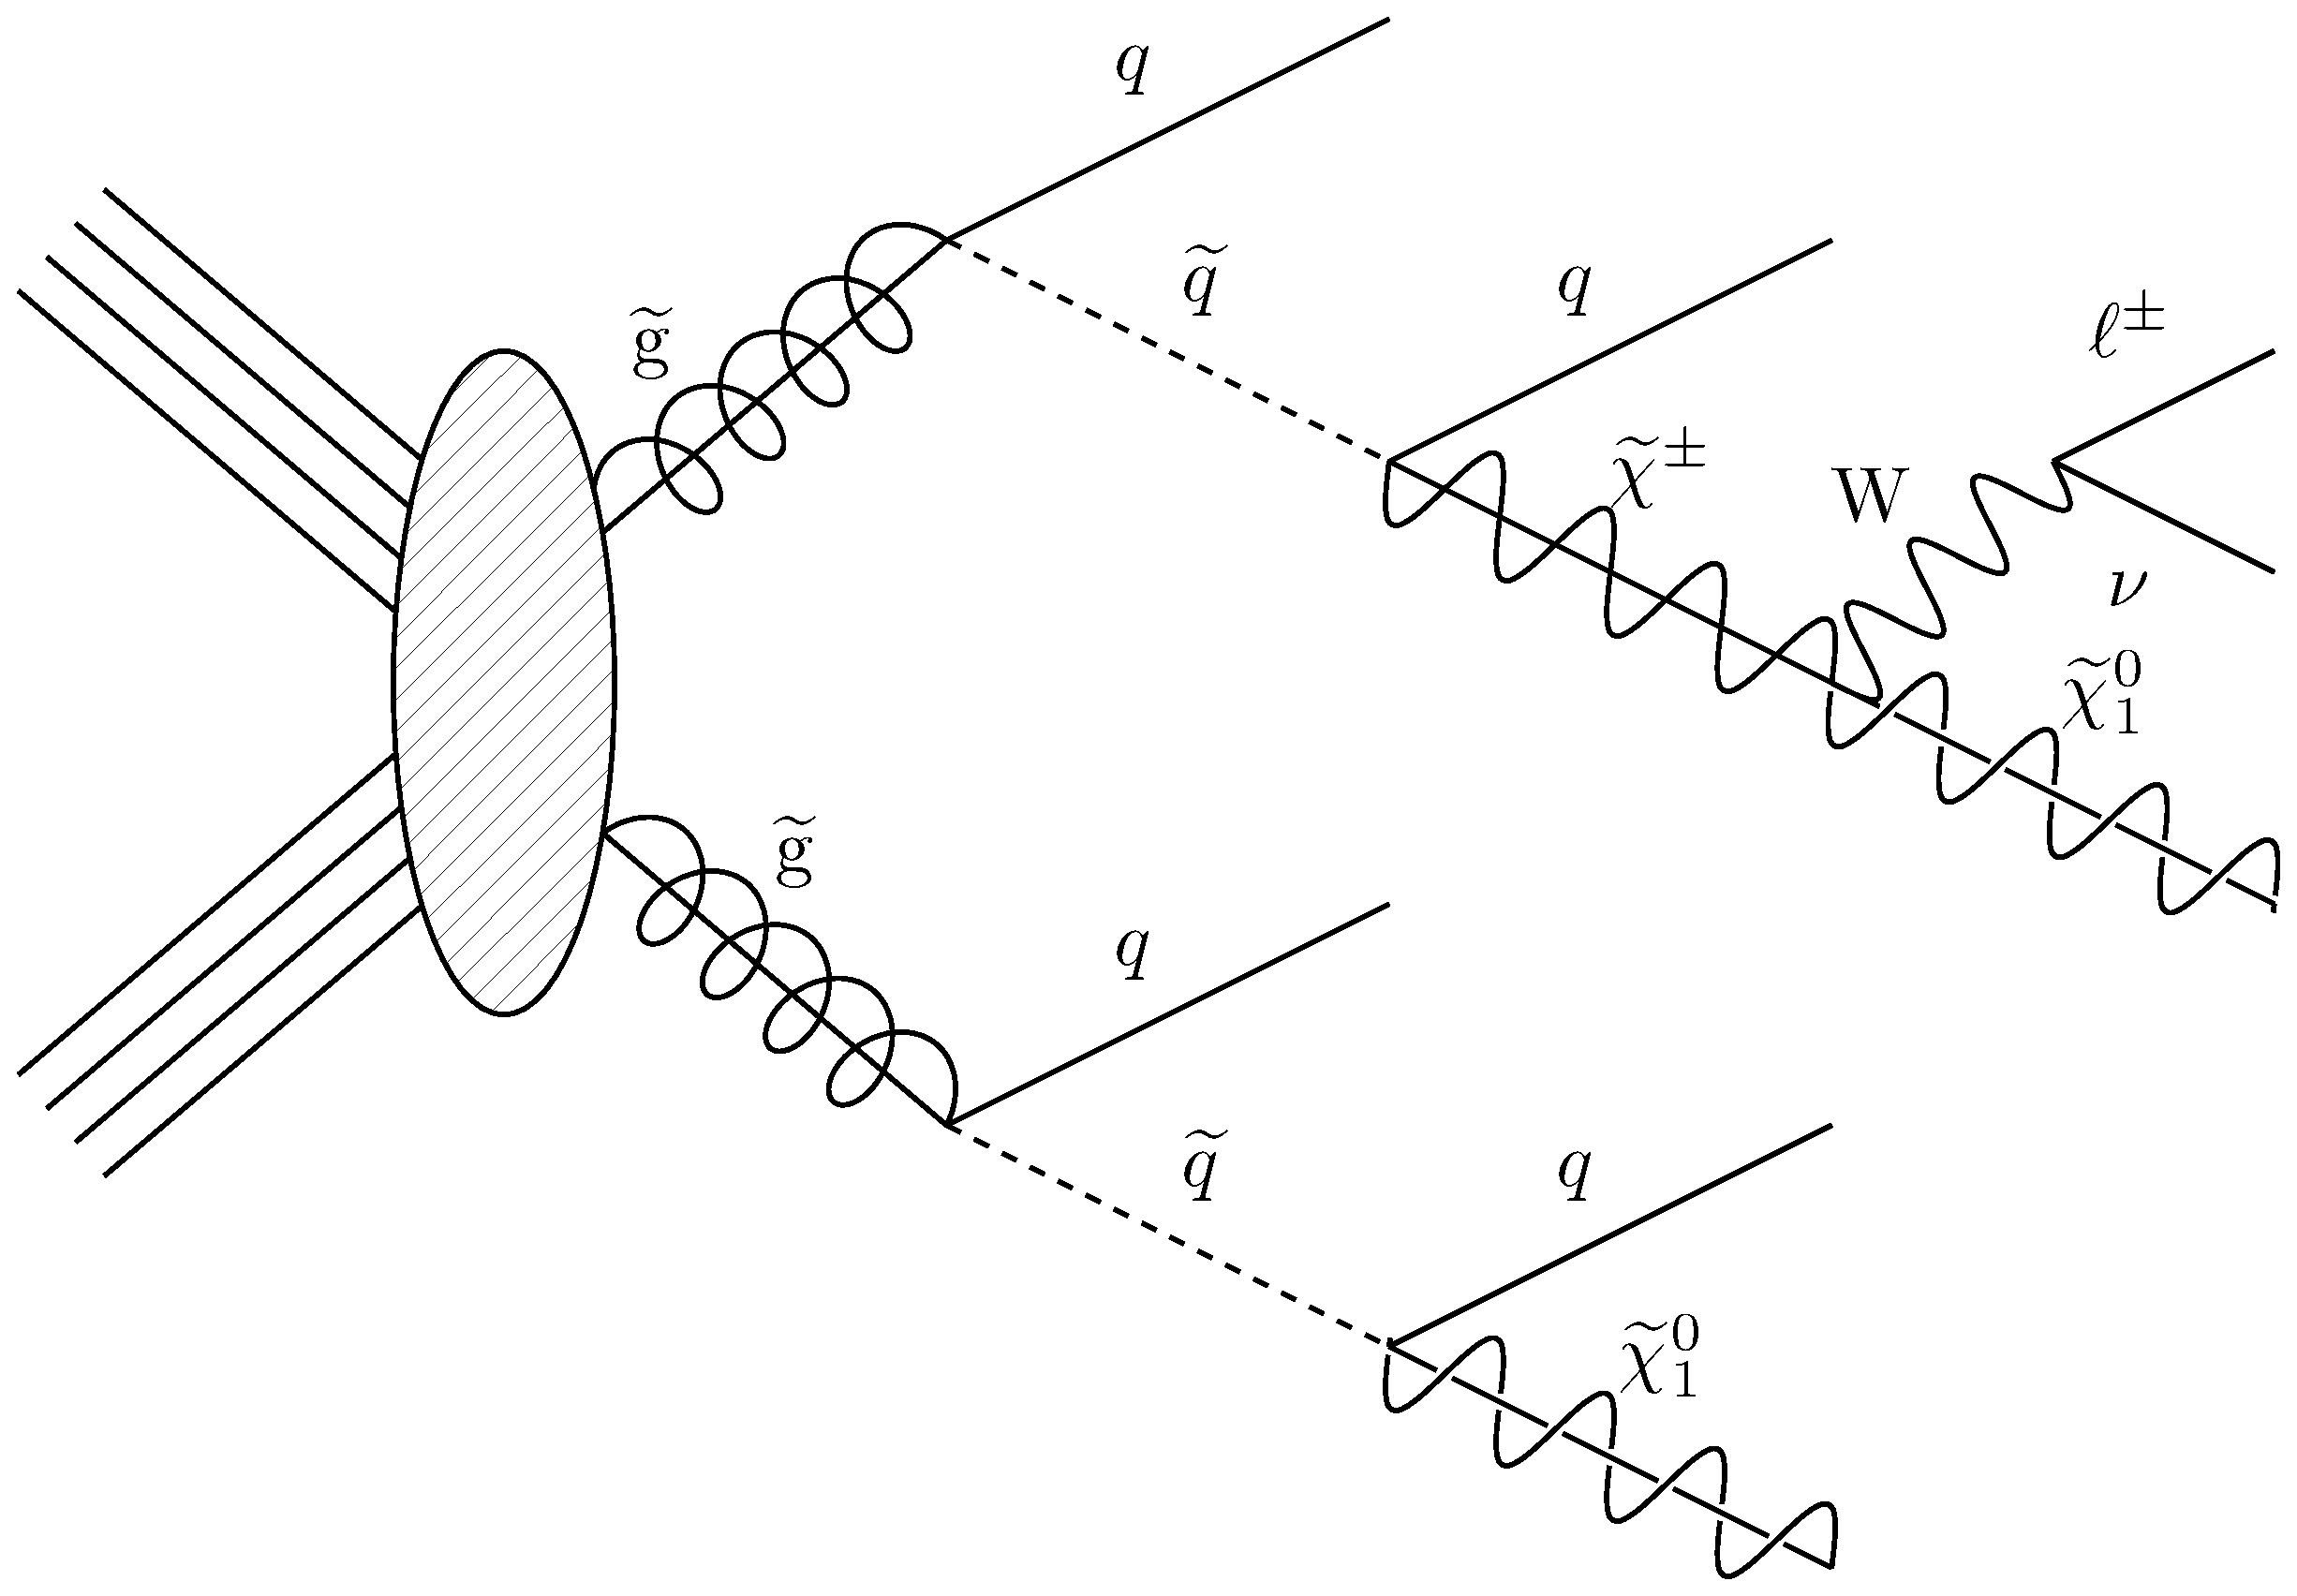
\includegraphics[width=0.7\textwidth]{fig/susy_1lep}
\caption[\ac{SUSY} decay chain leading to a single lepton final state]{Diagram
  showing a possible \ac{SUSY} decay chain beginning with gluino pair-production
  and leading to a single lepton final state.}
\label{fig:susy_1lep_decay}
\end{figure}

One such cascade decay is shown in \fig~\ref{fig:susy_1lep_decay}. This would be
a typical cascade decay leading to a single-lepton final state. Whilst being
less inclusive than the pure jets plus missing energy signature, the addition of
a lepton requirement serves to significantly suppress the experimental
background from \ac{QCD} events~\cite{msugra_signals}. With additional kinematic
requirements imposed, this channel is sensitive to a range of \ac{SUSY}
scenarios. A search based on this final state will be presented in
\chap~\ref{sec:susysearch}.

  \chapter{The CMS Experiment at the Large Hadron Collider}
\section{Introduction}
The Large Hadron Collider (LHC) is a proton-proton ($\Pp\Pp$) accelerator
located at the CERN particle physics laboratory near Geneva, Switzerland. The
LHC is built in the tunnels formerly occupied by the LEP experiment, a
\unit{27}{\kilo\metre} long ring lying on the border between France and Switzerland. Two
beams of protons run in opposite directions around the ring and are made to
collide at four interaction points.

There are four primary experiments at the LHC: \ac{ALICE}, \ac{ATLAS}, \ac{CMS}
and \ac{LHCb}. Each one is constructed around one of the four interaction points
and records the shower of particles produced from the colliding protons. ATLAS
and CMS are large, general purpose detectors designed to search for a variety of
\ac{NP} signatures as well as making higher precision measurements of \ac{SM}
parameters. \ac{ALICE} is designed to examine the products of heavy-ion
collisions (lead-lead) in order to explore the quark gluon plasma and related
physics. Finally, the \ac{LHCb} experiment is optimised for the study of B-meson
decays. These are important for the study of CP violation within the \ac{SM} but
might also provide potential avenues for the discovery of \ac{NP}.

In addition to the four larger detectors, two smaller experiments, \ac{LHCf} and
\ac{TOTEM} lie upstream of the \ac{ATLAS} and \ac{CMS} collision points in order
to probe more specialised forward physics phenomena.

\section{The \acl{LHC}}
The \ac{LHC} is a circular $\Pp\Pp$ synchrotron with a circumference of
\unit{27}{km}. It sits in a tunnel initially constructed for the \ac{LEP}
accelerator buried at a depth of between 50 and \unit{175}{\metre} beneath the
Franco-Swiss border. At full design specifications, 2808 bunches of protons will
circulate around each direction of the ring, colliding at a centre of mass
energy of \unit{14}{\TeV}. With a proton bunch spacing of
\unit{25}{\ns}, the \ac{LHC} will eventually achieve a luminosity of
\unit{$10^{34}$}{\rpsquare{\centi\metre}\usk\reciprocal\second}.

\subsection{Accelerator Complex}
The \ac{LHC} ring itself is the final stage in an injector chain utilising a
series of accelerators built at CERN over the last 50 years. Each stage supplies
an incremental increase in the proton (or heavy ion) bunch energy. The first
stage in this chain is a linear accelerator, either the Linac2 for proton
injection or Linac3 during heavy-ion runs. The Linac2 injects protons into the
\ac{PSB} at an energy of \unit{50}{\mega\electronvolt}. Similarly, the ions
proceed first from the Linac3 to the \ac{LEIR} before finally arriving at the
\ac{PS}. From here on, the paths of the protons and heavy-ions are the
same. Proton bunches pass from the \ac{PSB} to the \ac{PS} at an energy of
\unit{1.4}{\giga\electronvolt} and then on to the \ac{SPS} at an energy of
\unit{28}{\giga\electronvolt}. Protons then arrive at the \ac{SPS}, where they
circulate around a ring \unit{2}{\kilo\metre} in diameter, and increasing their
energy to \unit{450}{\giga\electronvolt}. From here, kicker magnets inject the
bunches into the \ac{LHC} itself, where the energy is finally increased to the
design specified \unit{7}{\TeV} per beam.
\begin{figure}
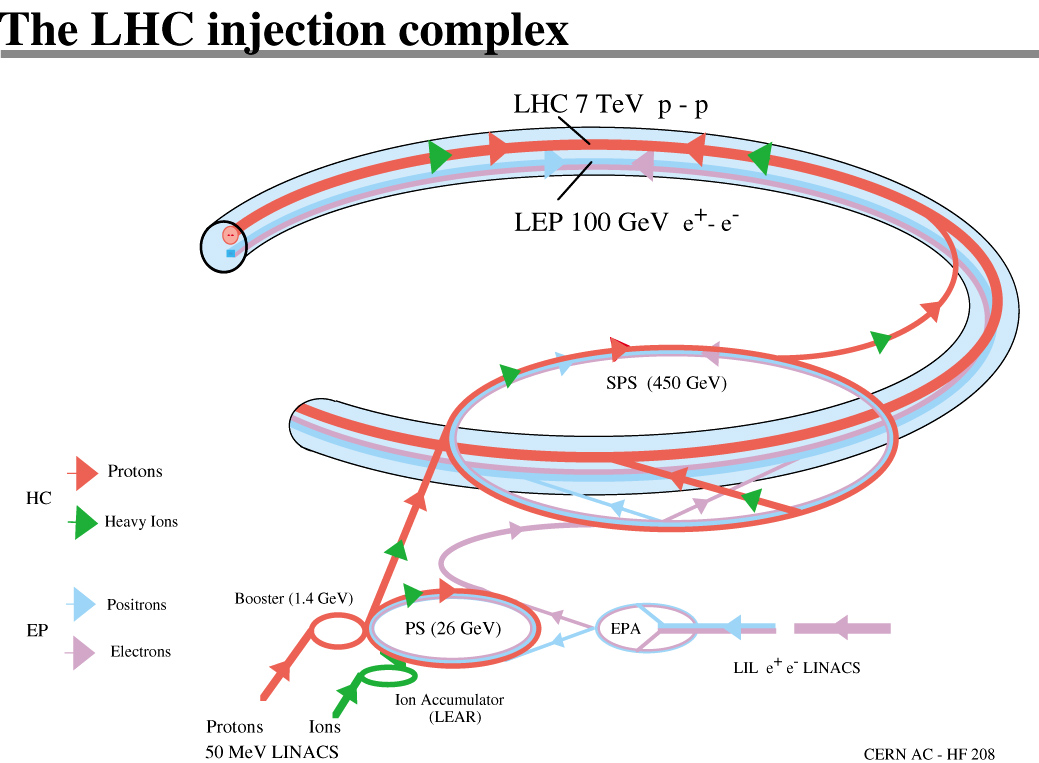
\includegraphics[width=0.9\textwidth]{fig/lhc-pho-1993-008}
\end{figure}

% TODO: More on the LHC beam etc.!

\ctable[
cap=LHC Accelerator Complex,
caption=LHC Accelerator Complex,
mincapwidth=0.5\textwidth,
pos=h
]{lcc}{
\tnote[a]{Heavy-Ions only}
}{\FL
Accelerator & Energy \ML
%
Linac2   & \unit{50}{\mega\electronvolt} \NN
Linac3\tmark[a]   & \unit{4.2}{\mega\electronvolt\per u} \ML
%
\acf{PSB} & \unit{1.4}{\giga\electronvolt} \NN
\acf{LEIR}\tmark[a]   & \unit{??}{\mega\electronvolt\per u} \ML
%
\acf{PS} & \unit{28}{\giga\electronvolt} \NN
\acf{SPS} & \unit{450}{\giga\electronvolt} \NN
\acf{LHC} & \unit{7}{\tera\electronvolt} \LL
}


\section{The \acl{CMS} Experiment}
\label{sec:cms}
\ac{CMS} is a large, general purpose detector\cite{cms_jinst} designed to firmly establish or
disprove the existence of the Higgs boson particle as well as performing
searches for a wide variety of \ac{NP} signatures. The design goals of CMS were
as follows (paraphrasing Design proposal):
\begin{enumerate}
\item a high quality, redundant muon system,
\item the best possible \ac{ECAL}
\item high quality central tracking to complement these two systems
\item an affordable detector
\end{enumerate}

These goals motivated the design of a traditional cylindrical detector,
\unit{21.5}{\metre} in length and \unit{15}{\metre} in diameter. A key feature
of the design is the \unit{4}{\tesla} superconducting solenoid. The bending
field supplied provides accurate muon momentum resolution up to energies of
\unit{$\approx$ 1}{\TeV}. The size of the solenoid placed stringent
limitations on the volume of the inner detector subsystems (everything except
for the muon chambers and return yoke).

\subsection{Coordinate System}
In order to facilitate discussion of the detector, a right-handed coordinate
system is defined with the origin chosen to be the nominal collision point
inside \ac{CMS}. The $x$ axis is then defined to point horizontally inwards
towards the centre of the \ac{LHC} ring and the $y$-axis vertically
upwards. Therefore the $z$-axis is aligned along the beamline pointing towards
the nearby Jura mountains. Often a cylindrical coordinate system will be used
with where the azimuthal angle $\phi$ and radial coordinate $r$ span the $x-y$
plane. The azimuthal angle is measured with respect to the $x$-axis. The
pseudorapidity, $\eta = - \ln \tan \frac{\theta}{2}$ where $\theta$ is the polar
angle measured with respect to the $z$-axis.

\subsection{Silicon Tracker}
The innermost subsystem of \ac{CMS} is the silicon tracker, designed to provide
highly precise measurements of particle trajectories close to the CMS
interaction point. The tracker extends to pseudorapidities of $|\eta|<2.5$ and
has an active silicon area of more than \unit{200}{\metre\squared} making it the
largest silicon tracker ever built.

The tracker design can be better understood by considering the expected particle
flux at design luminosity as a function of radial distance $r$ from the
beamline.

\begin{itemize}
\item At $ r \approx \unit{10}{\cm}$ the particle flux is highest. Accordingly,
  the innermost layer of the CMS tracker is comprised of hybrid pixels. With an
  area of \unit{$100\times 150$}{\micro\metre\squared}, particle densities are
  $O(10^{-4})$ per pixel per LHC bunch crossing.
\item At a radius \unit{$20 < r < 55$}{\centi\metre}, reduced particle flux allows
  the use of silicon microstrip sensors. With a much larger area of
  $\unit{10}{\centi\metre}\times\unit{80}{\micro\metre}$, average particle
  densities are $O(10^{-2})$ per strip per bunch crossing.
 \item At $ r > \unit{55}{\cm}$, the silicon strip size is once again increased
   to $\unit{25}{\cm}\times \unit{180}{\cm}$ again giving a particle density of
   $O(10^{-2})$ per strip per bunch crossing.
\end{itemize}

\subsubsection{Pixel Tracker}
The hybrid pixels are placed closest to the interaction point. As well as
maintaining an acceptable particle density per sensor, their close proximity to
the interaction point allows the origin of collision products to be accurately
determined. This is of particular importance for instance in B-tagging. In the
barrel region, 3 layers are placed at mean radii of 4.4, 7.3 and
\unit{10.2}{\cm}. The detector has a length of \unit{53}{\cm} in the $z$
direction. The end discs are instrumented with only two layers and are located
at $|z|=34.5, \unit{46.5}{\cm}$. The pixel modules in these layers are arranged
in a turbine-like layout.

To acheive the desired spatial resolution, the pixels have an almost square
geometry with an area of \unit{$150\times 100$}{\micro\metre\squared} in the
$r\phi\times z$ ($r\times r\phi$) for the barrel (end discs).

\subsubsection{Strip Tracker}
Further from the interaction point, the tracker is instrumented with silicon
strip detectors. The barrel component can be further divided into the \ac{TIB}
and the \ac{TOB}. The \ac{TIB} is composed of 4 layers with the \ac{TOB}
comprising a further 6. The \ac{TOB} extends to $z = \pm
\unit{118}{\centi\metre}$. Beyond this are the endcaps which can again be split
into two components: the \ac{TEC} made up of 9 disks and the \ac{TID} 3. The
silicon micro strip sensors are \unit{320}{\micro\metre} thick and oriented
parallel to the $z$ axis in the barrel and radially in the disks.

Both the \ac{TIB} and \ac{TID} supply up to four measurements of $r\phi$. With a
strip-pitch of \unit{80}{\micro\metre} in the inner two layers and
\unit{120}{\micro\metre} in the outer two, the \ac{TIB} achieves a single point
resolution of \unit{23 and 35}{\micro\metre} respectively. In the \ac{TID}, the
strip pitch varies between \unit{100 and 141}{\micro\metre}.

The \ac{TOB} uses \unit{500}{\micro\metre} thick sensors with a strip-pitch of
\unit{183}{\micro\metre} in the first four layers and \unit{122}{\micro\metre} in
the outer two. This gives a single point resolution of \unit{53}{\micro\metre}
and \unit{35}{\micro\metre} respectively.

The first two layers of the \ac{TIB}, \ac{TOB} and \ac{TID} and rings 1, 2 and 5
of the \ac{TEC} are so-called stereo modules. These are double-sided modules
where the two layers of strips have a stereo angle of \unit{100}{\milli\radian}
between them. This provides additional resolution in the $z$ measurement in the
barrel (or $r$ in the endcaps). The resolution of this measurement is
\unit{230}{\micro\metre} and \unit{530}{\micro\metre} in the \ac{TIB} and
\ac{TOB} respectively.

\begin{figure}
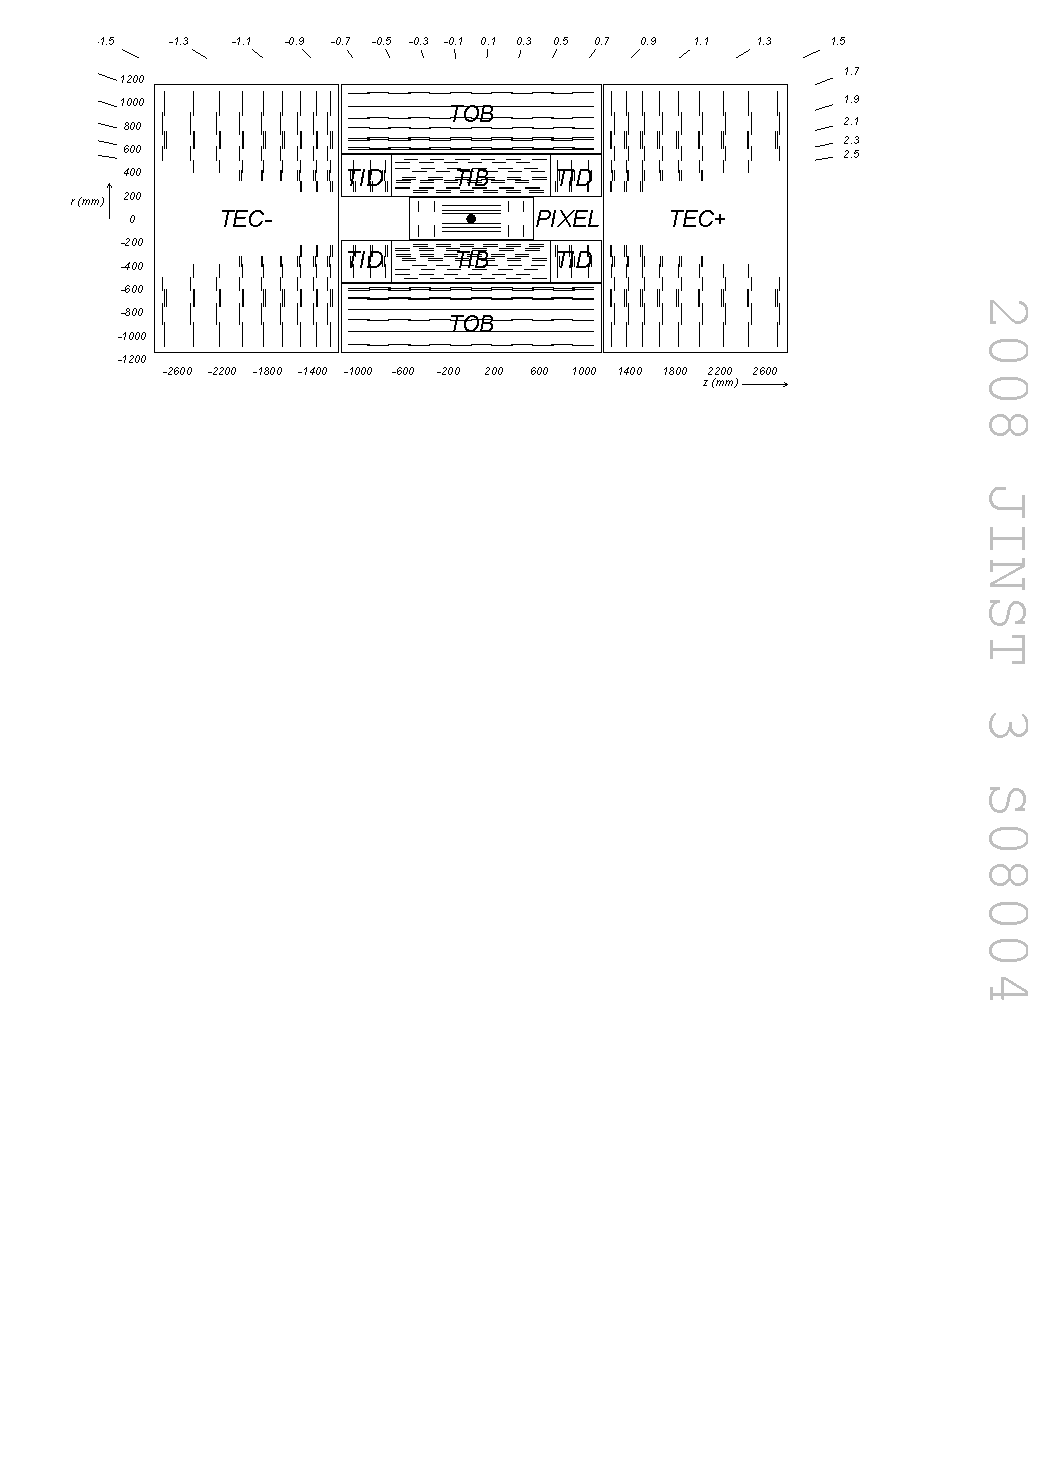
\includegraphics[width=\textwidth]{fig/tracker}
\end{figure}

\subsection{\acl{ECAL}}
The \ac{ECAL} surrounds the silicon tracker and provides a high resolution
measurement of electromagnetic showers within a homogeneous, hermetic
calorimeter composed of 61,200 lead tungstate (PbWO$_4$) crystals. This material
was chosen for its high desnity, short radiation length and small Moli\`{e}re
radius. Scintillation photons are then recorded by \ac{APD}s in the barrel and
\ac{VPT}s in the endcap. The driving motivation for the \ac{ECAL} design was the
detection of the low-mass favoured Higgs decay channel
$PH\longrightarrow\gamma\gamma$.

\subsubsection{\acl{EB}}
The \ac{EB} extends in rapidity to $|\eta|<1.479|$ with a crystal
segmentation of $360\times 85$ ($\eta-\phi$) in each half barrel. Each crystal
is slightly tapered with a cross-section of $0.0174\times0.0174$ in
$\eta-phi$. The crystals have a front cross section of \unit{$22\times
  22$}{\milli\metre\squared} and a length of \unit{230}{\milli\metre}
(corresponding to 25.8 radiation lengths).

\subsubsection{\acl{EE}}
The \ac{EE} occupies the rapidity range $1.479 < |\eta| < 3.0$. Crystals are
grouped into $5\times 5$ supercrystals within a carbon-fibre alveolar
structure. The endcaps are split into two halves, known as Dees, each holding
3,662 crystals.

The scintillation of the ac{ECAL} crystals as well as the amplification of the
\acp{APD} varies as a function of temperature. This variation was found to be
\unit{$\approx 4\%$}{\per\celsius}. For this reason, the \ac{ECAL} temperature
is precisely regulated to within \unit{$\pm$ 0.05}{\celsius}.

\subsubsection{Laser Monitoring System}
\label{sec:expt_laser_monitoring}
The PbWO$_4$ crystals that make up the \ac{ECAL} are raditation resistant but
quickly suffer a decrease in their optical transmission under irradiation. This
is a result of the formation of colour centres which absorb a fraction of the
incident light. At a working temperature of \unit{18}{\celsius}, the damage
anneals leading to an equilibrium in the optical transmission properties -
constant with dose rate. The consequence of this is a cyclic change in the
optical transmission rate of the crystals as the \ac{LHC} moves between
colliding beams and machine refills. Since this depends on dose rate, the effect
is a function of \ac{LHC} luminosity and rapidity. It is expected to range from
a shift of $\sim 2\%$ in the barrel at low luminosity to $> 10\%$ in the endcaps
at high luminosity. The magnitude of this effect on energy and momentum
measurements would be disastrous if not properly accounted for. Correction of
the reconstruction necessitates constant monitoring of the transparency - a task
performed by the laser monitoring subsystem. The corrections itself will be
discussed further in the context of the electron reconstruction (see
Section~\ref{sec:reco_ecal_transparency}).

Three lasers are used for the transparency measurement: two blue ($\lambda
\approx \unit{440}{\nano\metre}$) and one near-infrared ($\lambda \approx
\unit{796}{\nano\metre}$). The blue laser (with a second fitted for redundancy
purposes) is close to the scintillation emission peak and thus can be used to
track the changes in the crystal transparency. The near-infrared laser is far
from the emission peak and thus relatively stable to changes in the
transparency. This can be used to verify the stability of the system. The lasers
are distributed to the crystals via optical fibre and a series of
fanouts. Approximately 1\% of the \ac{LHC} beam gap of
\unit{3.17}{\micro\second} is used for transparency monitoring. A full scan of
the entire \ac{ECAL} can be achieved in approximately 30~minutes. The lasers can
be pulsed at $\approx \unit{80}{\mega\hertz}$ with a pulse timing jitter of
\unit{3}{\nano\second}. This is adequate for synchronisation with the \ac{LHC}
bunch crossings and \ac{ECAL} \ac{ADC} clock.

The transparency of the crystals is derived from the response of the \ac{APD}
normalised to the height of the laser pulse, as measured using a silicon \ac{PN}
photodiode. Due to differences in path length and optical spectra between the
laser and the scintillation light, the transparency of the crystals may be
related to the measured transparency via a power law.


\subsection{\acl{HCAL}}
Accurate measurement of hadronic showers is crucial for analyses involving jets
or missing energy type signatures. The \ac{HCAL} lies between the outer edge of
the ECAL and the inner edge of the solenoid ($\unit{1.77}{\metre} < r <
\unit{2.95}{\metre}$). This constrains the size of the \ac{HCAL} to a relatively
compact design and necessitates the placement of a ``tail catcher'' outside of
the solenoid.

\subsubsection{\acl{HB}}
\subsubsection{\acl{HE}}


\subsection{Magnet}
\subsection{Muon Chambers}
As has already been said, sensitive detection of muons is one of \ac{CMS}'s key
design goals. Since the effect of radiative losses in the tracker is much less
for muons than it is for electrons, muons are able to provide a much finer mass
resolution which can be used in a variety of physics searches and
measurements. The muon system at CMS is responsible for muon identification,
momentum measurement and triggering (for further detail see
Section~\ref{sec:trigger}). Three types of detectors are used, chosen for
different regions of the detector according to the magnetic field, muon rate and
response time required for input to the trigger.

\subsubsection{\acl{DT}}
In the barrel region, the magnetic field is relatively uniform and the muon flux
low enough to allow the use of drift tubes. These identify muons in the region
$|\eta| < 1.2$. The drift chamber was first developed as a refinement of earlier
wire proportional chamber designs in which the drift time of the electrons to
the anode wire is used to provide additional spatial resolution. This allows the
wire spacing to be increased thus reducing the electronics requirements.

Each drift chamber is composed of 2 (or 3) superlayers, which are further
divided into 4 layers of rectangular drift cells. Of the four concentric muon
stations in the barrel, the inner three contains 60 drift chambers and the
outermost 70. The wires in the outer two layers of each drift cell are oriented
parallel to the beam line, providing a measurement in the $r\phi$ direction (the
magnetic bending plane). The inner two layers are perpendicularly aligned,
giving a measurement of the $z$ coordinate.

\subsubsection{\acl{CSC}}
In the endcap region, the large muon and background rate coupled with the large,
non-uniform magnetic field prevent the use of \ac{DT}s. Instead, \acl{CSC}s are
used. The CMS Muon endcap consists of 468 \ac{CSC}s, each a trapezoidal
multiwire proportional chamber arranged radially covering an azimuthal angle
$\Delta\phi$ of either 10 or 20 degrees. Each \ac{CSC} is a multiwire
proportional chamber with 6 anode wire planes interleaved with 7 cathode strip
planes. The wire readout provides a measurement of the $\phi$ coordinate whilst
$r$ position information is obtained by interpolating charges on the cathode
strips.

\subsubsection{\acl{RPC}}
In order to provide a fast trigger signal (see Section~\ref{sec:trigger}), a
muon detector capable of providing a fast signal is required. This is the
\acl{RPC}, a gaseous parallel-plate detector with spatial resolution suitable
for both barrel and endcap regions and a response time much less than the
\unit{25}{\nano\second} between consecutive \ac{LHC} bunch crossings.

\subsection{Data Aquisition and Trigger System}
\label{sec:trigger}
The high luminosity at the \ac{LHC} brings with it a large particle flux. Along
with the requirements of precise position and momentum measurements, this has
motivated the fine granularity present across each \ac{CMS} subdetector. The
natural consequence of this is an extremely large number of readout channels,
approximately 55 million across the whole detector. To make matters
worse, it is planned that the \ac{LHC} will eventually reach a bunch spacing of
only \unit{25}{\nano\second}. This places a tight latency requirement on the
\ac{DAQ} system.

Tightly coupled to the \ac{DAQ} is the trigger system. The huge number of
readout channels in \ac{CMS} is not only a problem in terms of the bandwidth of
the \ac{DAQ} but also poses serious problems relating to long-term storage
requirements. A digited, zero-supressed event dump from \ac{CMS} is
approximately \unit{2}{\mega\byte} in size. With an event rate of upto
\unit{40}{\mega\hertz}, this would potentially require a storage rate of
\unit{80}{\tera\byte\per\second}. Even with the rapid improvement of disk
storage technology over the last few decades, such storage capacities are
clearly infeasible both in terms of capacity and \ac{IO} requirements. For these
reasons, a system capable of quickly rejecting a very large fraction of
collisions is required. This is known as the trigger.

  \chapter{Physics Objects}

\section{Electrons}
\subsection{\ac{ECAL} Transparency Corrections}
\label{sec:reco_ecal_transparency}
  \chapter{Measuring the Helicity Polarisation of the $\PW$ Boson}
\section{Introduction}
The study of \Wjets production at a hadron collider presents an important
opportunity for furthering understanding of the underlying Electroweak and
\ac{QCD} processes. In particular, since it is one of a relatively small number
of processes for which highly precise \ac{NLO} calculations have been performed,
experimental measurements can give a direct constraint on the \acp{PDF}. \Wjets
production is also of considerable interest in the context of \ac{NP} searches
where these events are often a dominant background. Finally, the neutrino in the
leptonic decay mode provides a source of ``real'' missing energy which can be
useful in the understanding of detector effects relevant to searches for
\acs{WIMP}-type particles present in \ac{SUSY} and other theories.

\section{Background}
Some theoretical background relating to \PW helicity effects has been presented
in Section~TODO. Here, the discussion will be oriented towards a more
experimental context.

For small values of \PW transverse momentum, \PtW the differential angular
cross-section for the process
$\Pp\Pp\longrightarrow\PWpm\longrightarrow\Plpm\Pgnl$ follows the Drell-Yan
distribution
\begin{equation}
\frac{dN}{d(\cos\theta)} \propto (1\mp \cos\theta)^2
\end{equation}

It is well known from straightforward helicity arguments\cite{mirkes_w_1994}that
\PW produced along the beam axis will exhibit a 100\% left-handed polarization. This
can be seen by considering the leading order partonic subprocesses
\begin{equation}
\Pup\APdown \longrightarrow \PWp \qquad\textrm{and}\qquad
\Pdown\APup\longrightarrow\PWm
\end{equation}
Firstly, note that the fraction of the proton momentum carried by the quark (as
determined by the \aclp{PDF}) is greater than that of the anti-quark. In
addition given that the \ac{LHC} is a $\Pp\Pp$ collider, valence anti-quarks are
not present. Anti-quarks must be drawn from the sea and are therefore likely to
be low momentum. Taking these two facts together, the quark is very likely to be
higher momentum than the anti-quark. By momentum conservation, it is expected
that the \PW will be produced overwhelmingly in the direction of the original
quark. Then given the \VminusA nature of the weak interaction, it is seen that
the quark must be left-handed and, by helicity conservation the \PW will be
polarised nearly 100\% left-handedly along the beam axis. A small dilution will
occur in instances where the anti-quark has by chance a larger momentum fraction
than the quark.

It is worth mentioning that the situation is not identical at the Tevatron
$\Pp\Pap$ collider. Although the \PWp also possess a 100\% left-handed
polarisation along the beamline (via similar arguments to those given above),
the \PWm are found to have a near 100\% right-handed polarisation. This is a
result of the subprocess $\APup\Pdown\longrightarrow\PWm$ where this time the
\APup carries more momentum.

In the case, where the \PW carries a significant transverse momentum \PtW, the
situation is more complex.


\begin{figure}
\centering
\subfloat[]{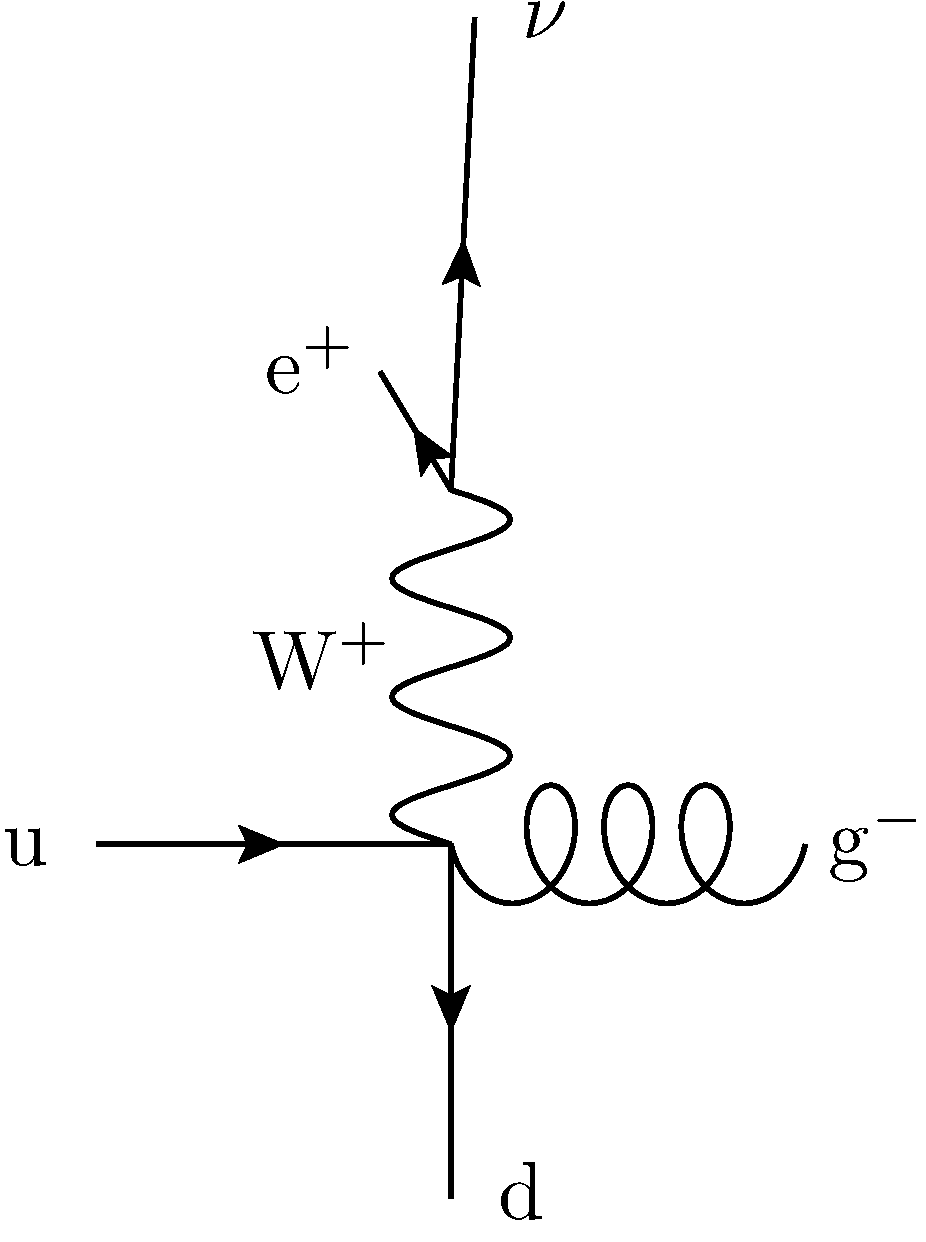
\includegraphics[width=0.3\textwidth]{fig/wpol_prod_a}}\quad
\subfloat[]{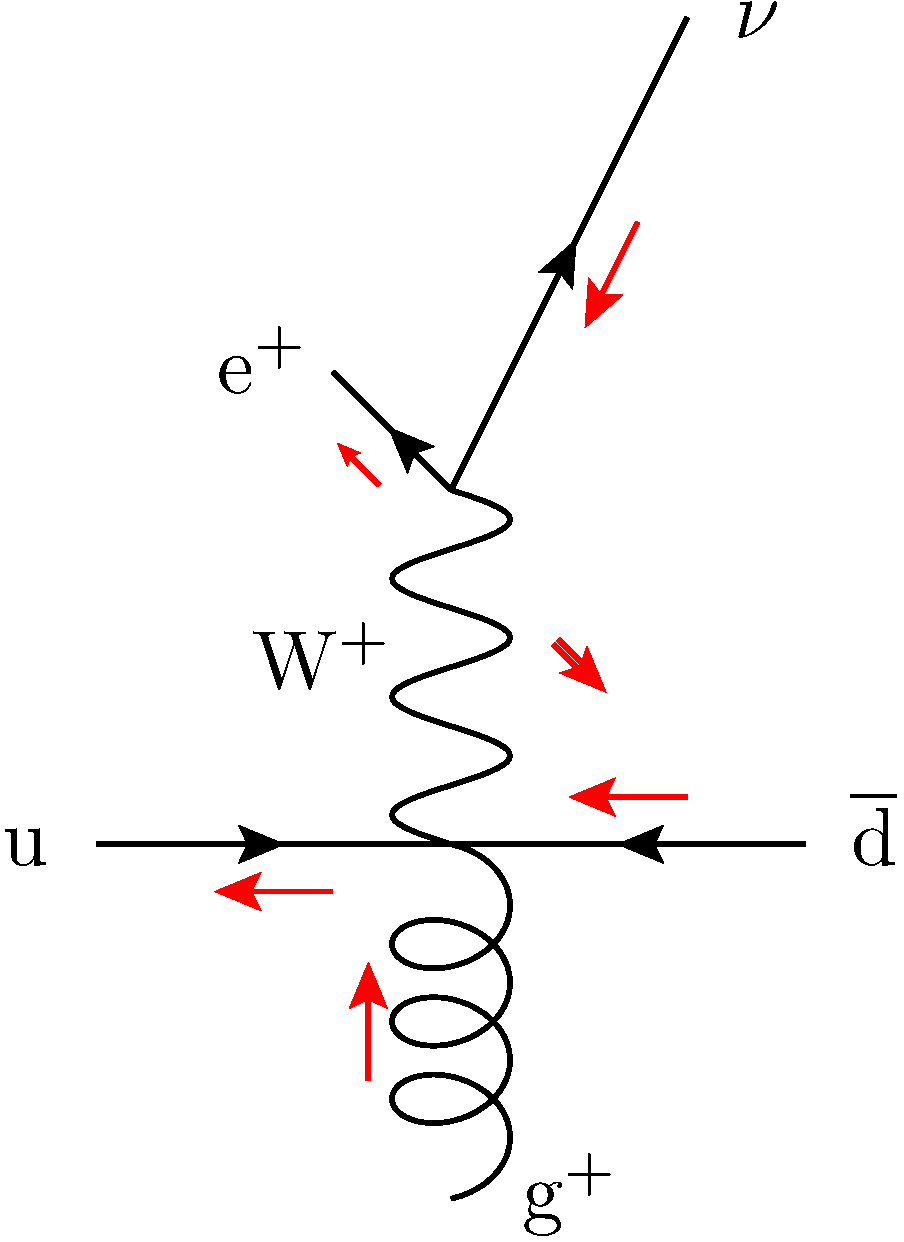
\includegraphics[width=0.3\textwidth]{fig/wpol_prod_b}}\quad
\subfloat[]{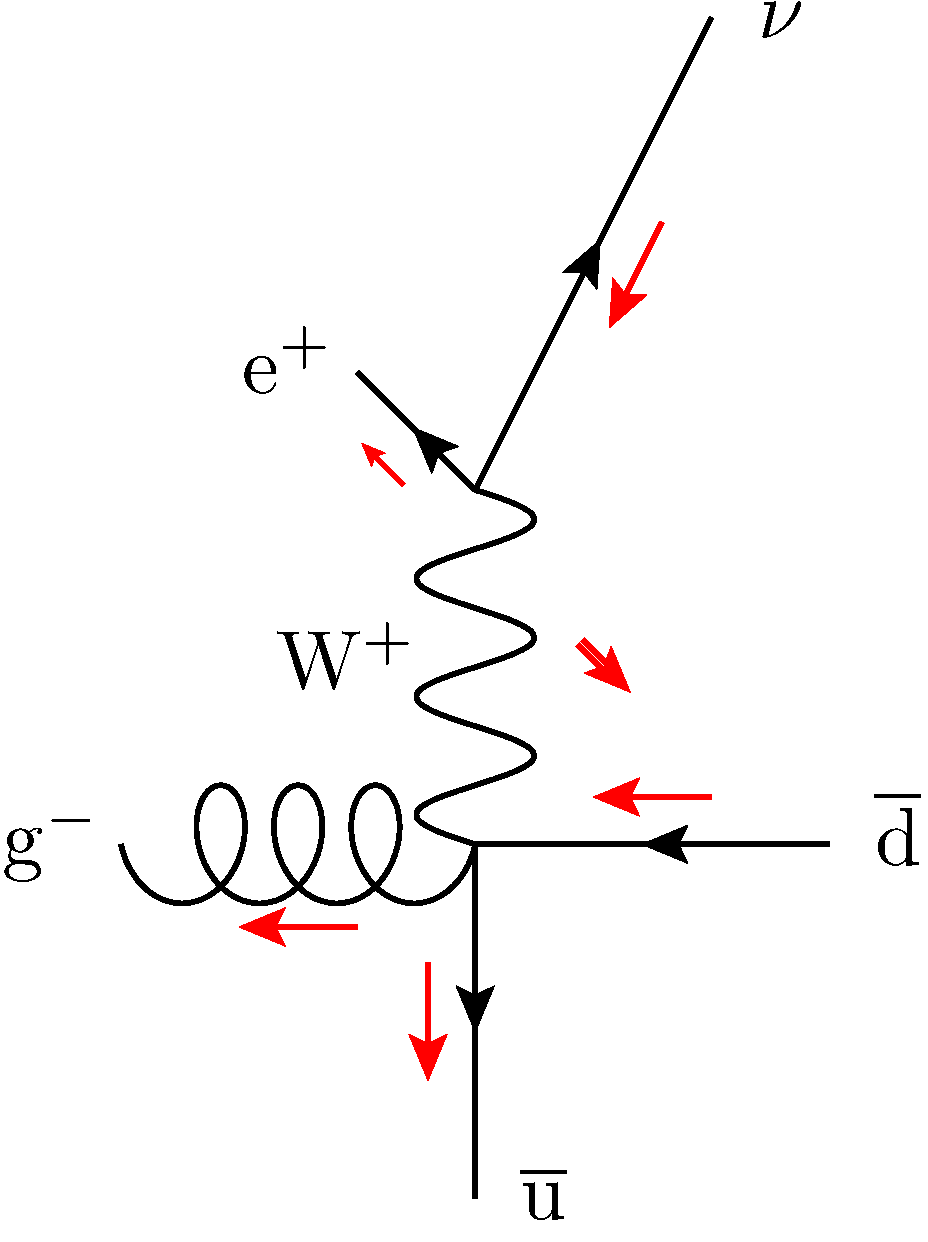
\includegraphics[width=0.3\textwidth]{fig/wpol_prod_c}}\\
\subfloat[]{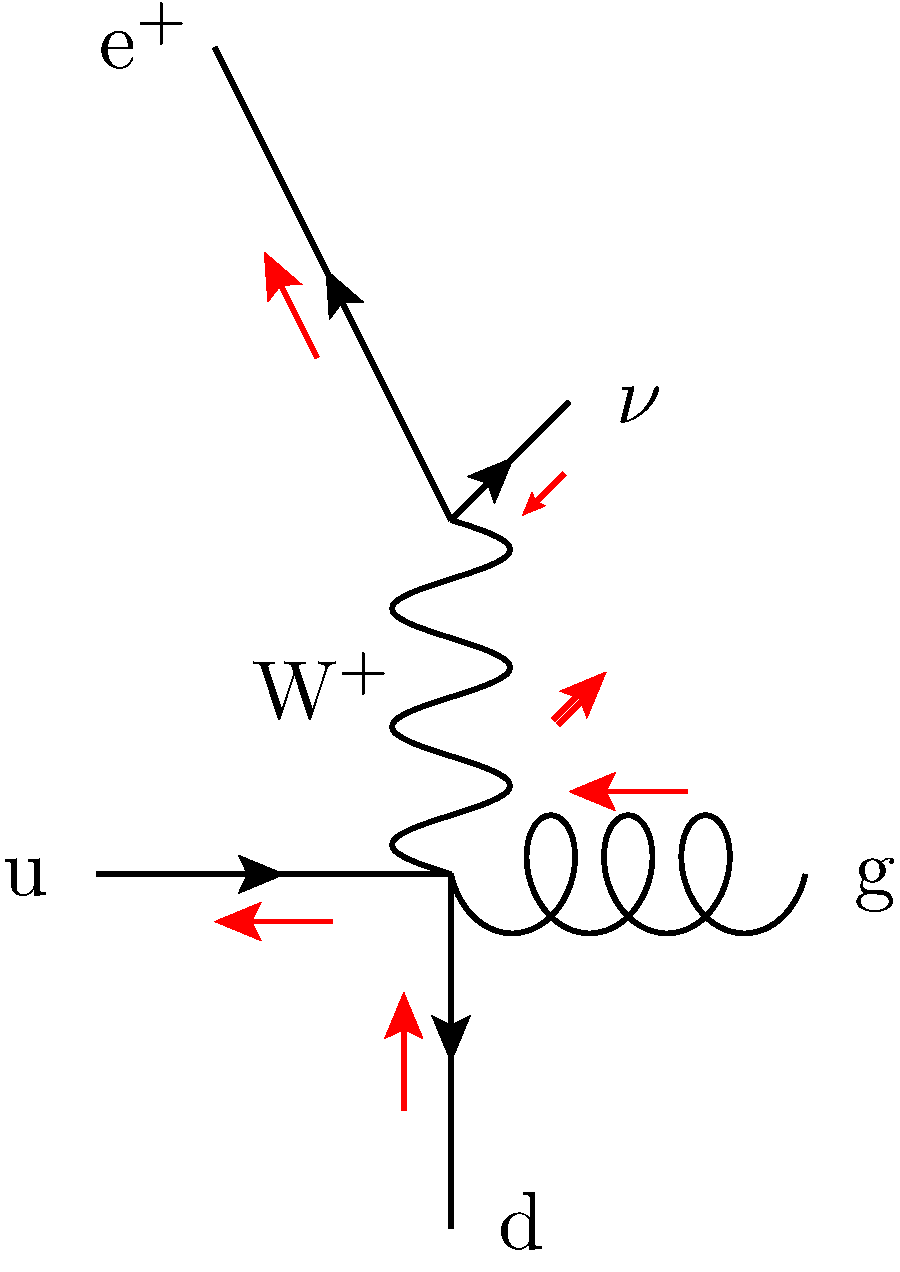
\includegraphics[width=0.3\textwidth]{fig/wpol_prod_d}}\quad
\subfloat[]{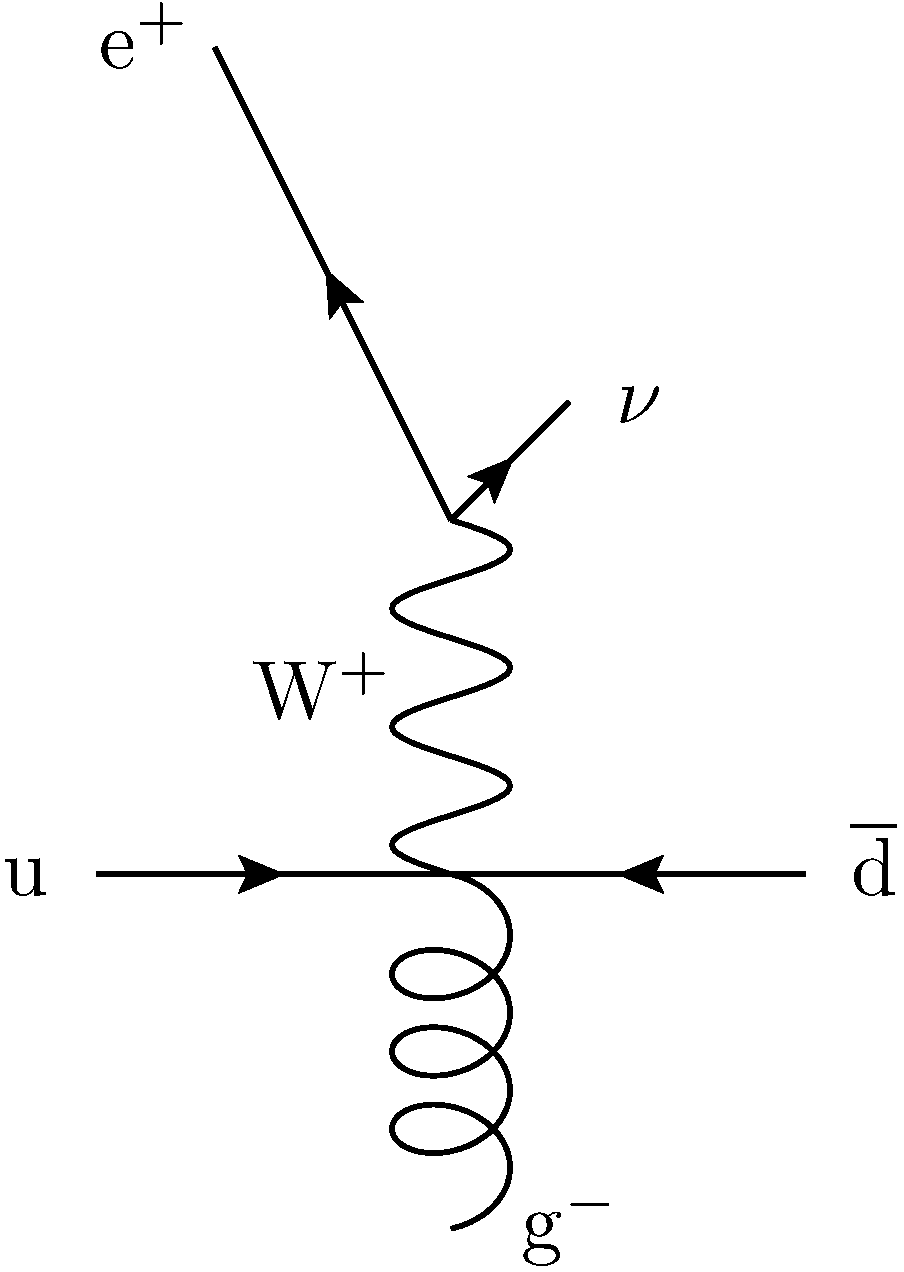
\includegraphics[width=0.3\textwidth]{fig/wpol_prod_e}}\quad
\subfloat[]{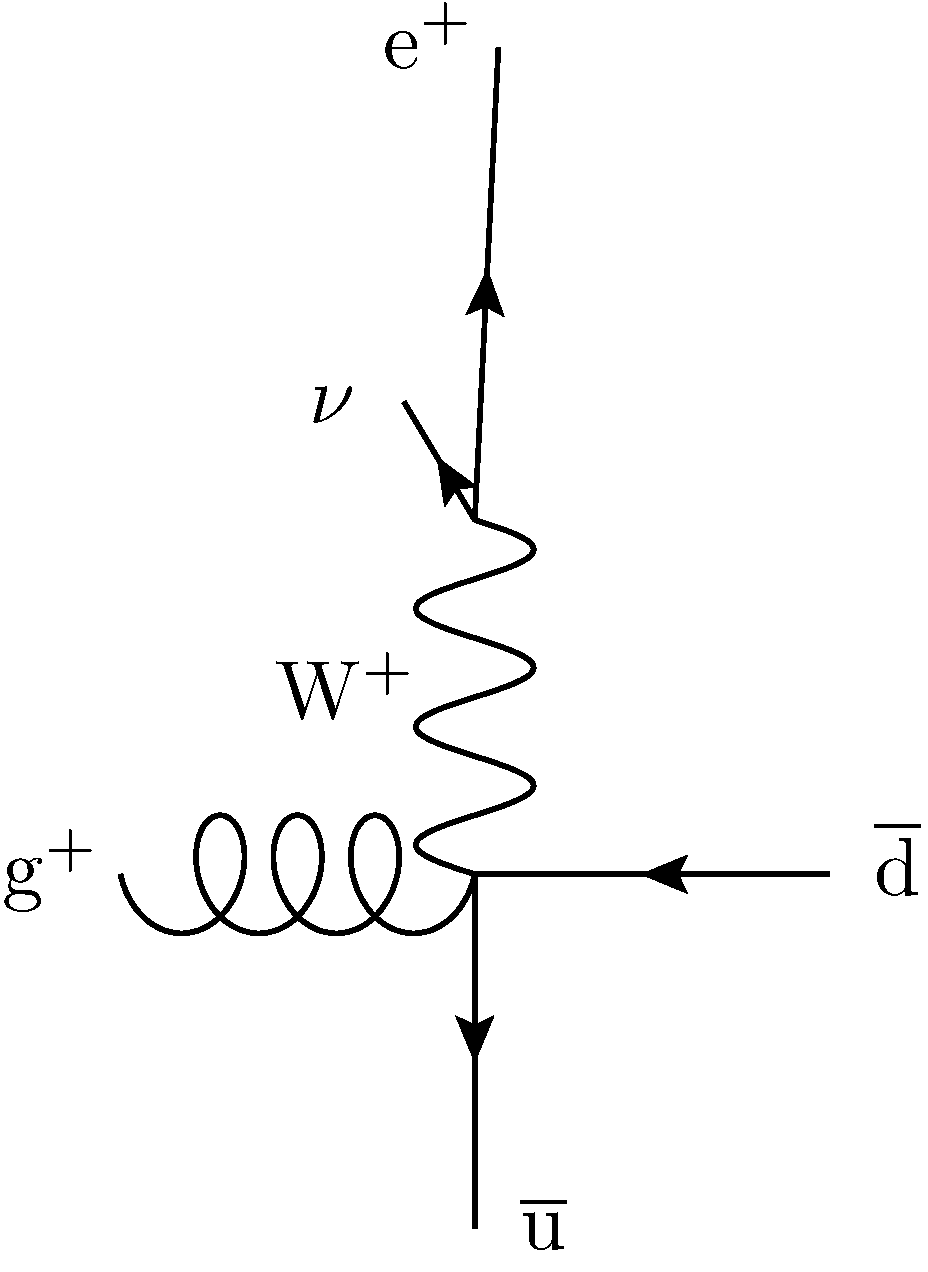
\includegraphics[width=0.3\textwidth]{fig/wpol_prod_f}}
\caption{Illustrations of $\PWplus+1$~jet production modes at the LHC. The
  $\Pgluon$ superscript indicates its helicity}
\label{fig:w1jet_modes}
\end{figure}
  \chapter{Searching for Supersymmetry in the Single Lepton Channel at CMS}
\section{Introduction}
The \PW polarisation measurement, as well as being an interesting analysis in
its own right, also finds application to searches for \acl{NP}. The first of
these, comes from a more complete understanding of the \MET distribution in
\Wjets events - an important background to many \ac{SUSY} searches. The second,
is that the polarisation of the \PW coupled with the methods described in the
previous chapter provides a means to discrimate \ac{SUSY} events from \ac{SM}
backgrounds. This will be further explored in the following section.

\section{Separating \as{SUSY} and \ac{SM} Events}
\label{sec:susy_sm}
In the context of \Rparity conserving \ac{SUSY}, a typical event with a charged
lepton in the final state is expected to contain 3 invisible particles: two
\acp{LSP} and a neutrino. As a result, the total \MET in an event will often be
larger than the transverse momentum of the charged lepton and relatively
uncorrelated with it in terms of direction. In contrast, the large boost and
polarisation of a typical \PW decay lead to a more even balance between the \MET
and the transverse momentum of the charged lepton, as well as greater
correlation of their directions. These two consideration can be applied to both
\Wjets and \ttbar events - the two dominant backgrounds to a single lepton
\ac{SUSY} search.

In order to make use of the \PW polarisation effects described, this analysis
makes use of the \LP variable as described in Section~\ref{sec:wpol_lp}. For
events containing a charged lepton and \MET originating from a \PW decay with
large transverse momentum, the alignment of the charged lepton and neutrino
gives an \LP distribution confined to the range $[0,1]$. In contrast, for
\ac{SUSY} events the \MET component is larger than the lepton momentum and thus
the \PtW is likely to point in the direction of the \MET. Since the direction
of the charged lepton momentum and \MET will be mostly uncorrelated, \LP is
likely to tend to small values. Rewriting,
\begin{equation}
\LP = \frac{\Ptl}{\PtW}\cos\left(\PtW, \Ptl\right)
\end{equation}
it can be seen that in cases where the angle between the \MET and \Ptl is more
than 90\degrees, \LP will become negative.

 A second important difference between \ac{SUSY} and
\ac{SM} events is related to the overall energy scale of the events. As
discussed in Chapter~\ref{sec:susy}, \ac{SUSY} decays are expected to begin with
initial states much heavier than in \ac{SM} events. To provide some measure of
this energy scale without biasing the polarisation, the variable \STlep is
constructed as follows,
\begin{equation}
\STlep = |\Ptl| + |\MET|
\end{equation}
where it should be noted that \STlep is a scalar quantity. For \PW decays,
$\STlep \approx \PtW$. Since the energy scale of \ac{SUSY} is unknown, \STlep is
used to define search regions. This allows the search to be optimised without
introducing a strong dependence on the energy scale. For the purposes of this
analysis, 4 \STlep bins are employed. These are: $150 < \STlep < 250$, $250 <
\STlep < 350$, $350 < \STlep < 450$ and $\STlep > \unit{450}{\GeV}$. The lowest
region, $\STlep_{150}$ is taken to be at too low an energy scale to contain
\ac{SUSY} processes not excluded by previous searches. It is used as a sideband
to validate the analysis method.

\section{Analysis Method}
The \LP distributions for \ac{SM} backgrounds and two benchmark \ac{SUSY} models
are shown in Figure~\ref{fig:susy_lp}. Firstly it can be seen that the heuristic
discussion of the \LP shape given in Section~\ref{sec:susy_sm} is confirmed by
the full simulation with \ac{SM} events giving $\LP > 0$ and \ac{SUSY} events
clustering around $\LP \sim 0$.
\begin{figure}
\centering
\subfloat[]{\label{fig:susy_lp_el_st250}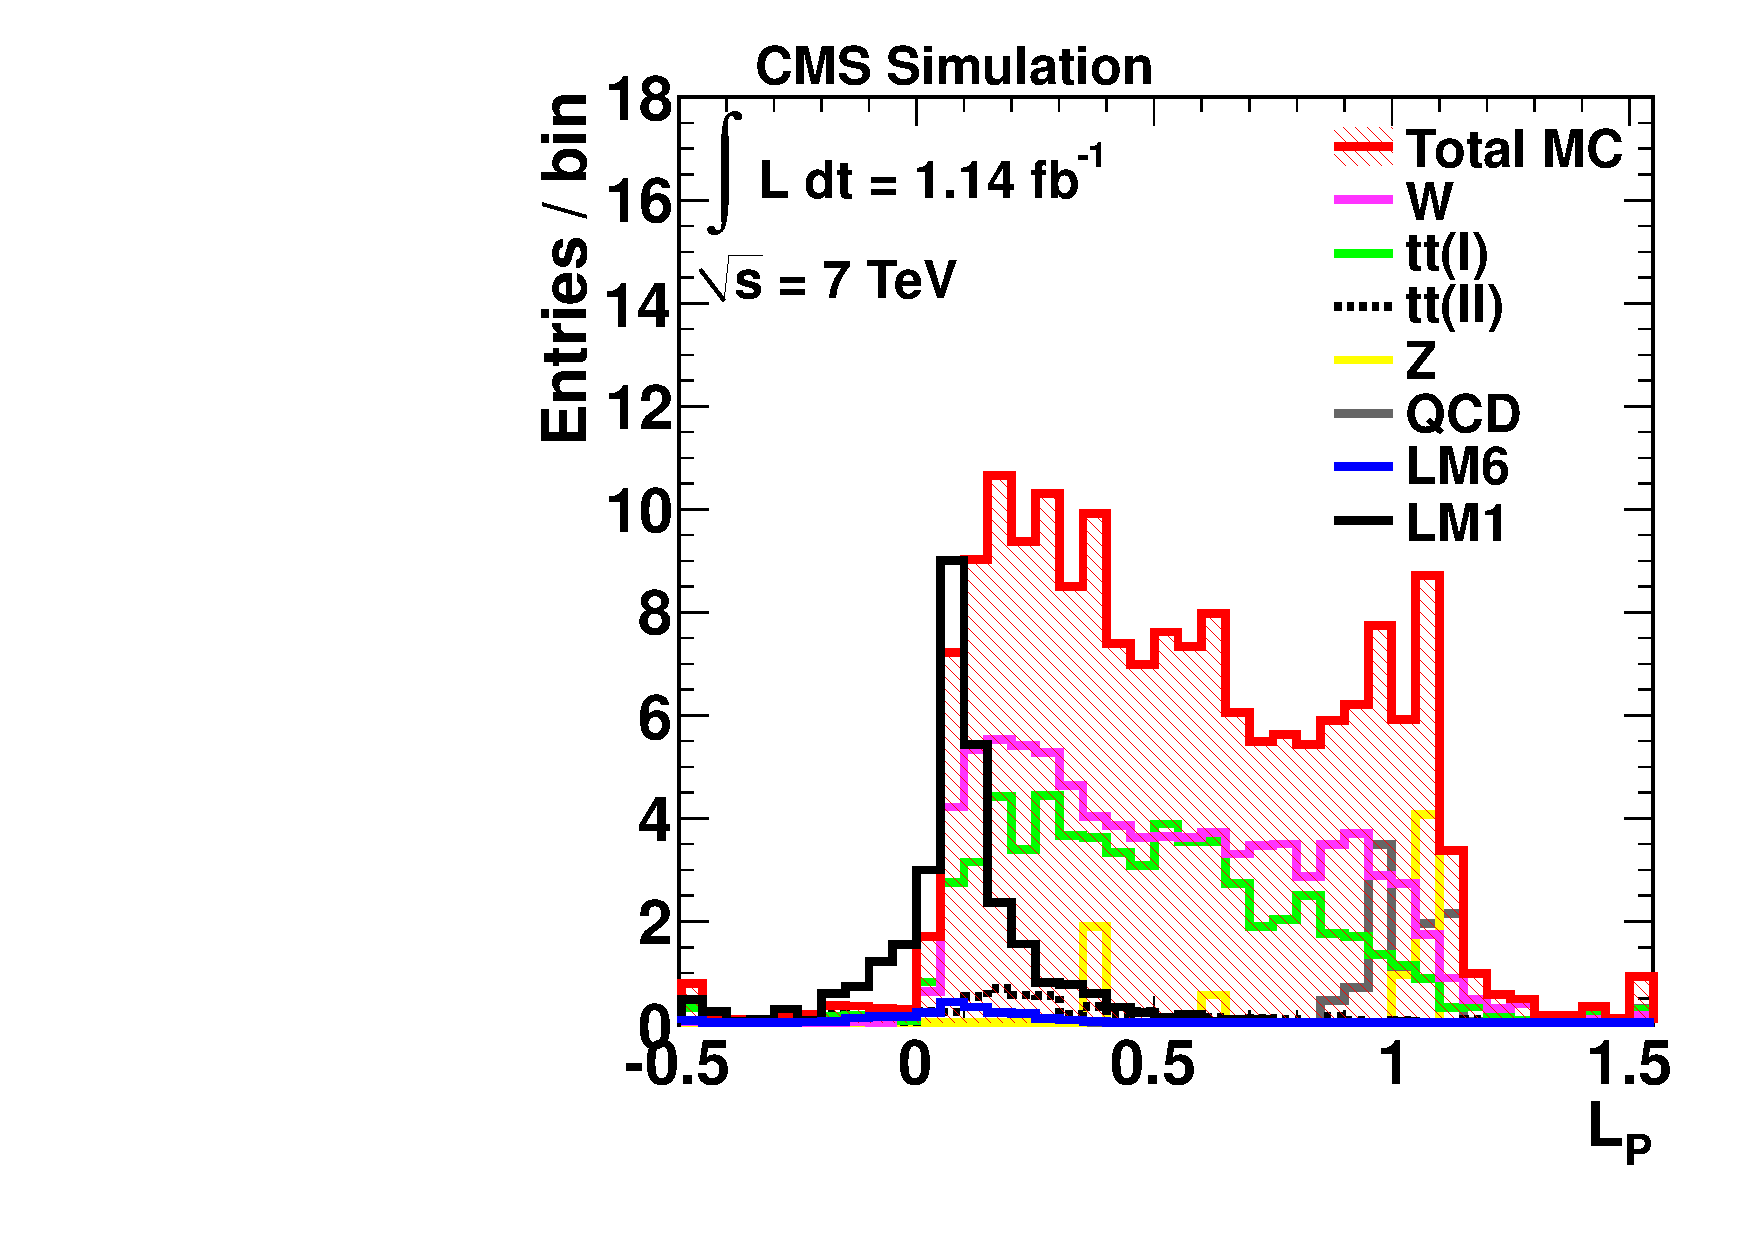
\includegraphics[width=0.3\textwidth]{fig/LP250_MCandSignal_El.pdf}}\quad
\subfloat[]{\label{fig:susy_lp_el_st350}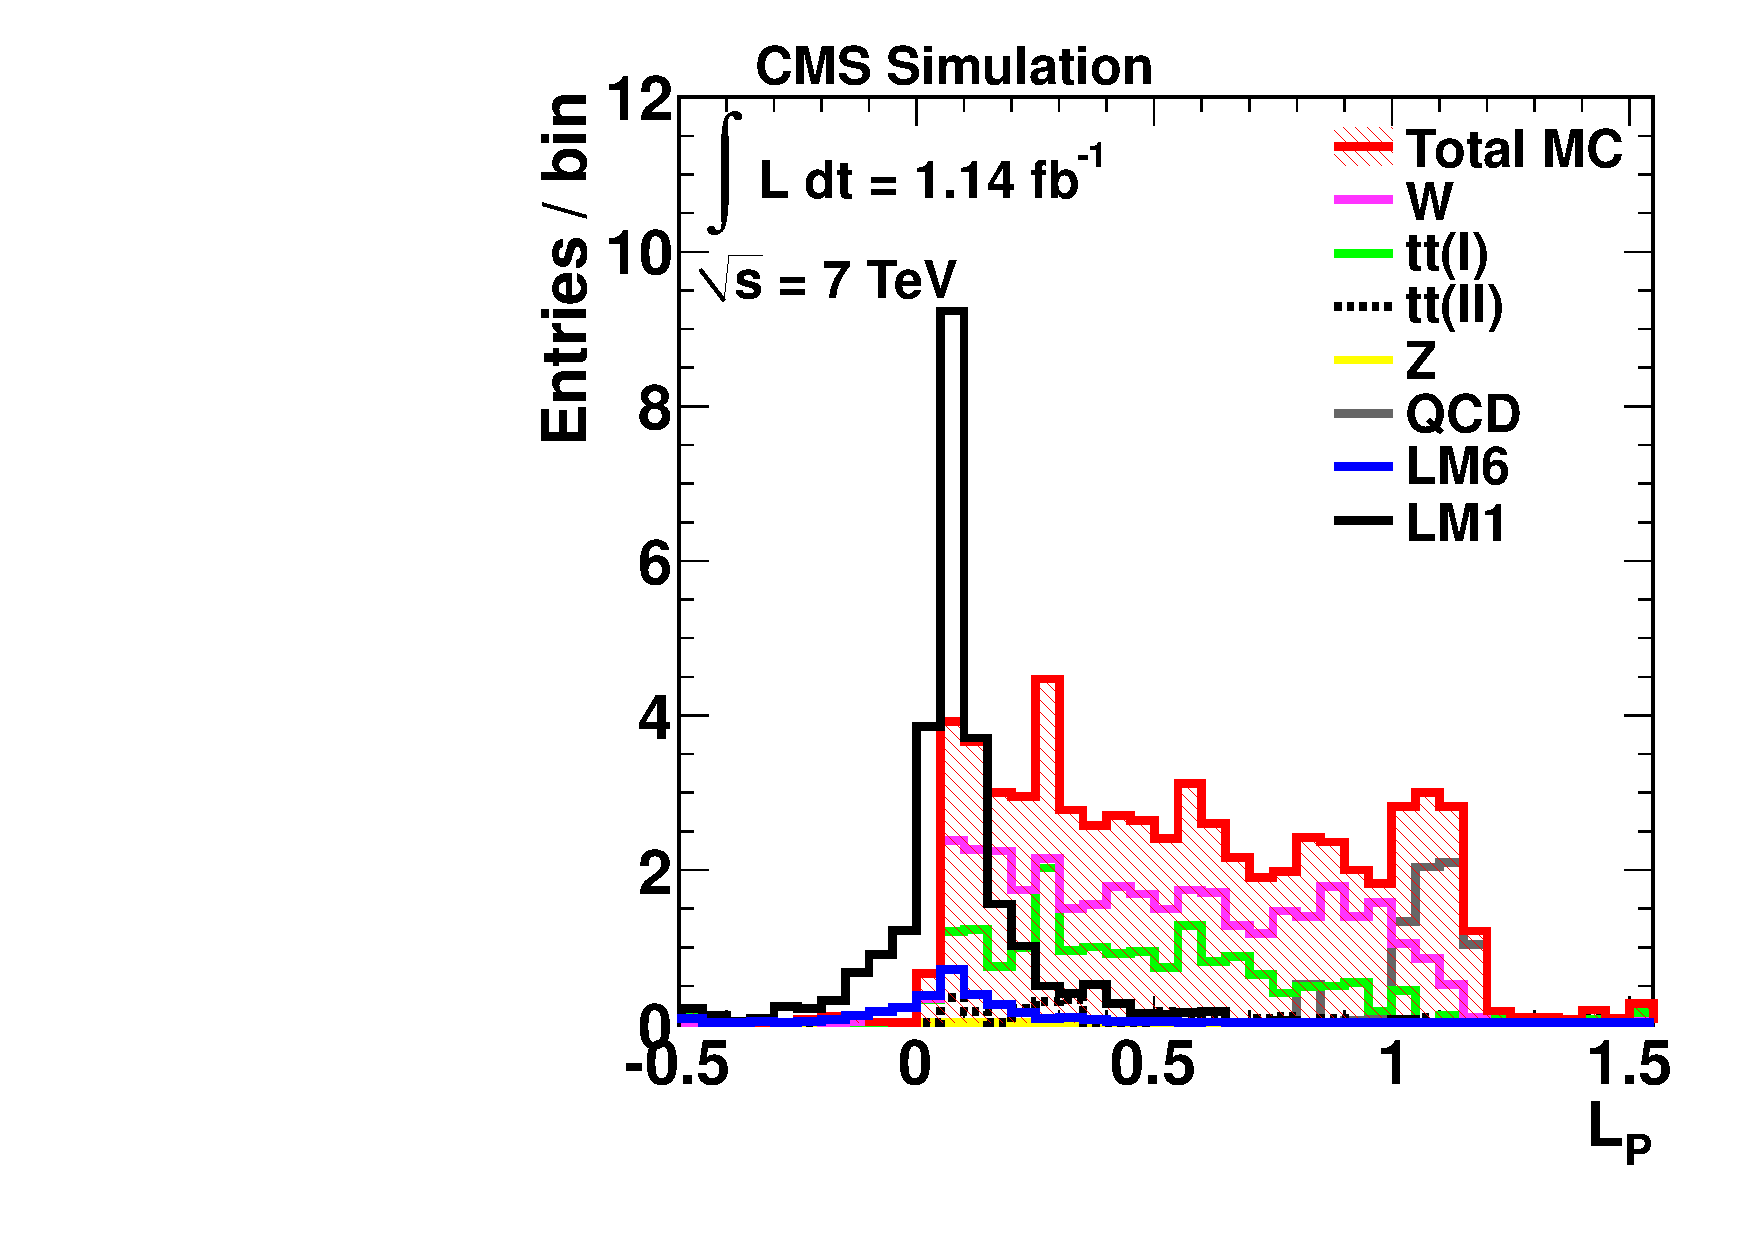
\includegraphics[width=0.3\textwidth]{fig/LP350_MCandSignal_El.pdf}}\quad
\subfloat[]{\label{fig:susy_lp_el_st450}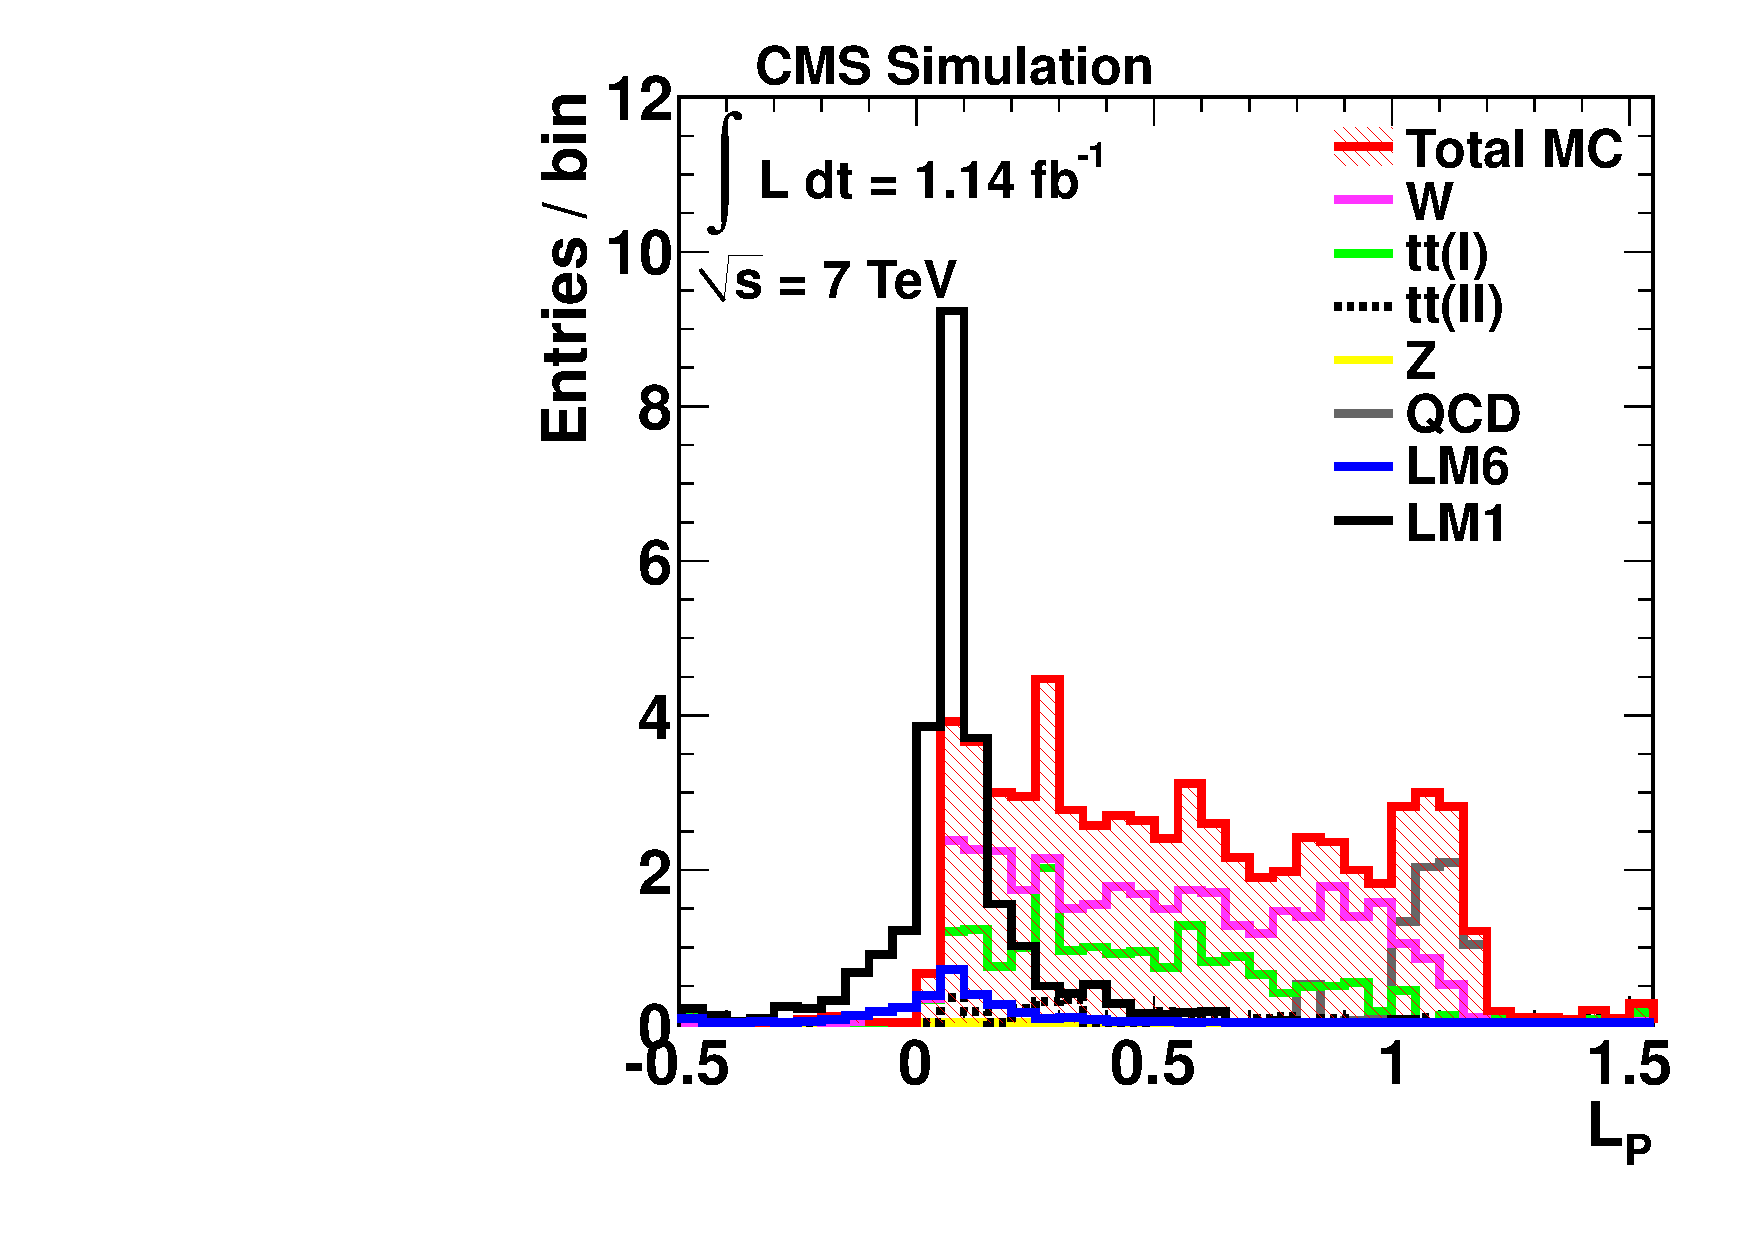
\includegraphics[width=0.3\textwidth]{fig/LP350_MCandSignal_El.pdf}}\\
\subfloat[]{\label{fig:susy_lp_mu_st250}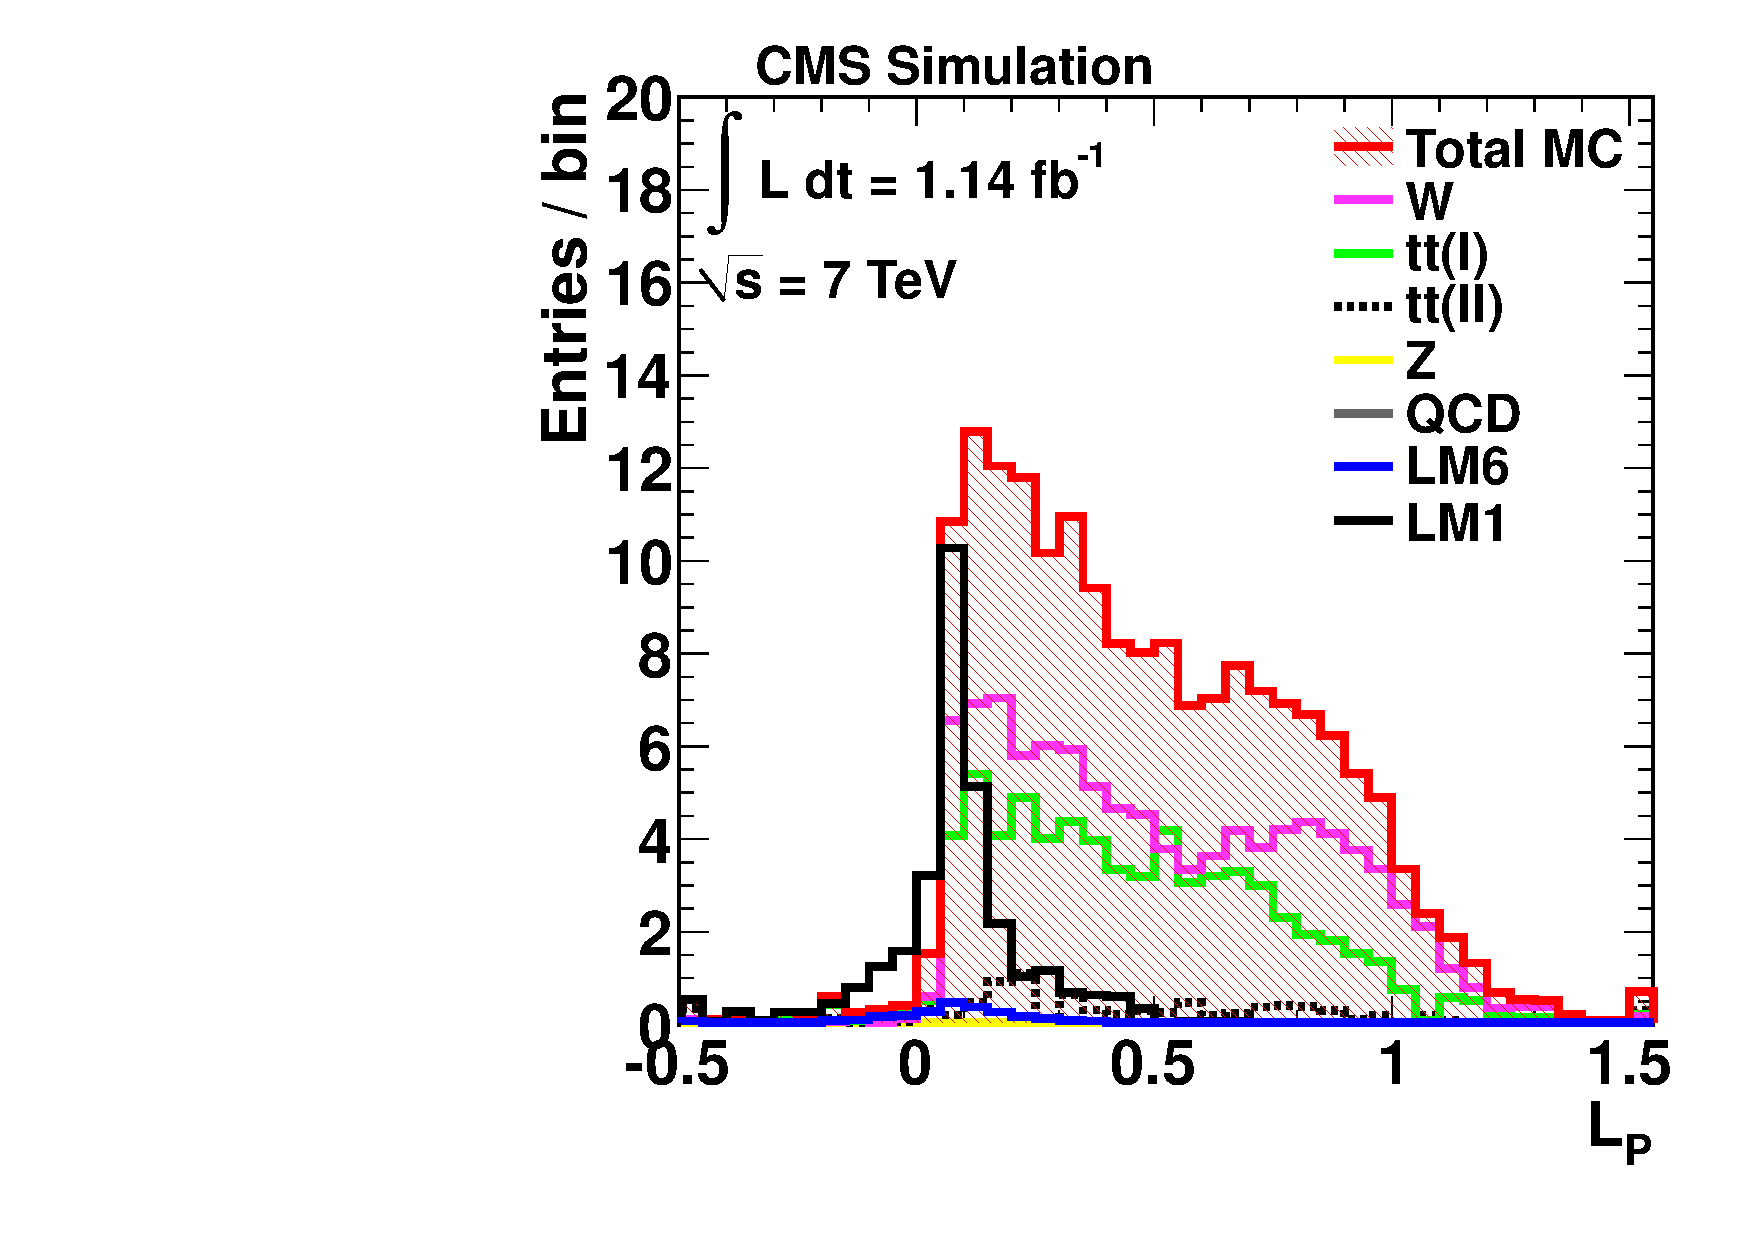
\includegraphics[width=0.3\textwidth]{fig/LP250_MCandSignal_Mu.pdf}}\quad
\subfloat[]{\label{fig:susy_lp_mu_st350}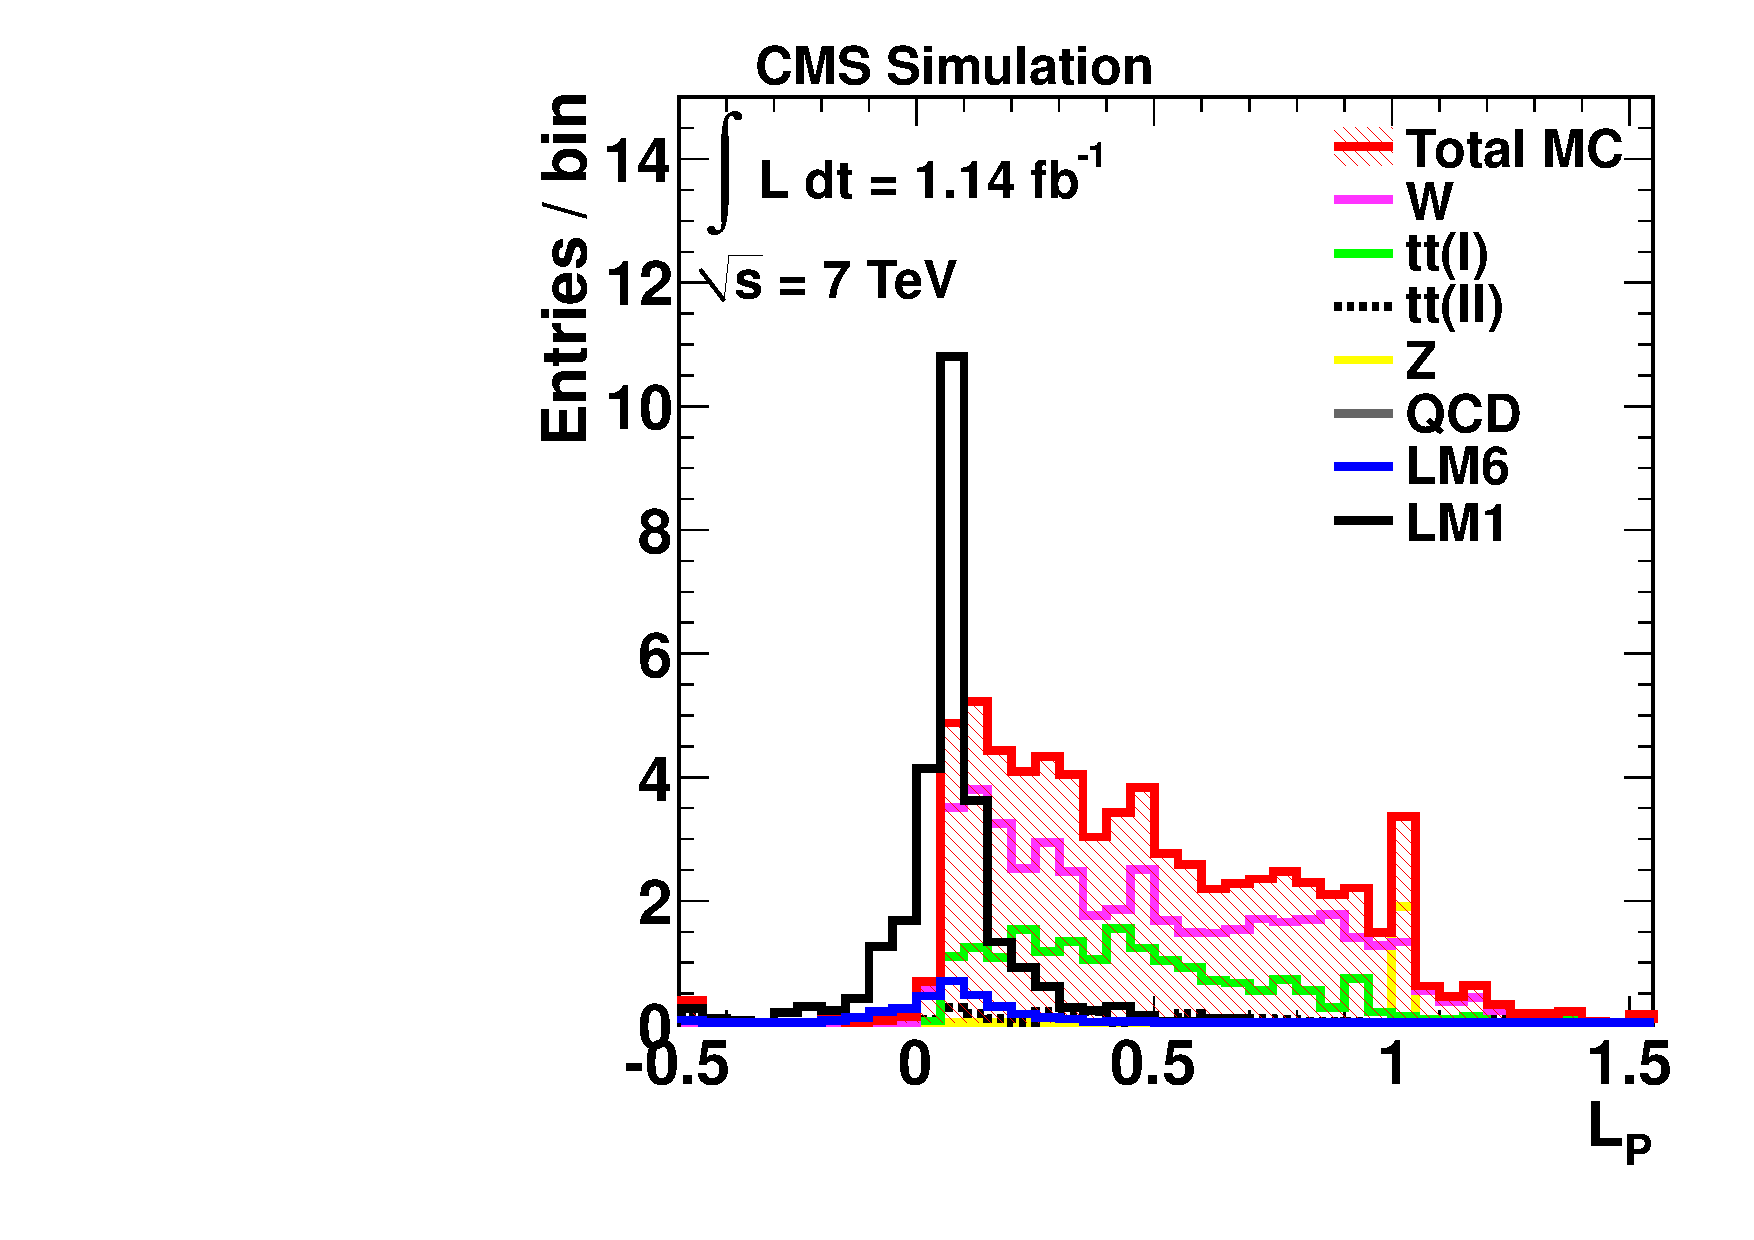
\includegraphics[width=0.3\textwidth]{fig/LP350_MCandSignal_Mu.pdf}}\quad
\subfloat[]{\label{fig:susy_lp_mu_st450}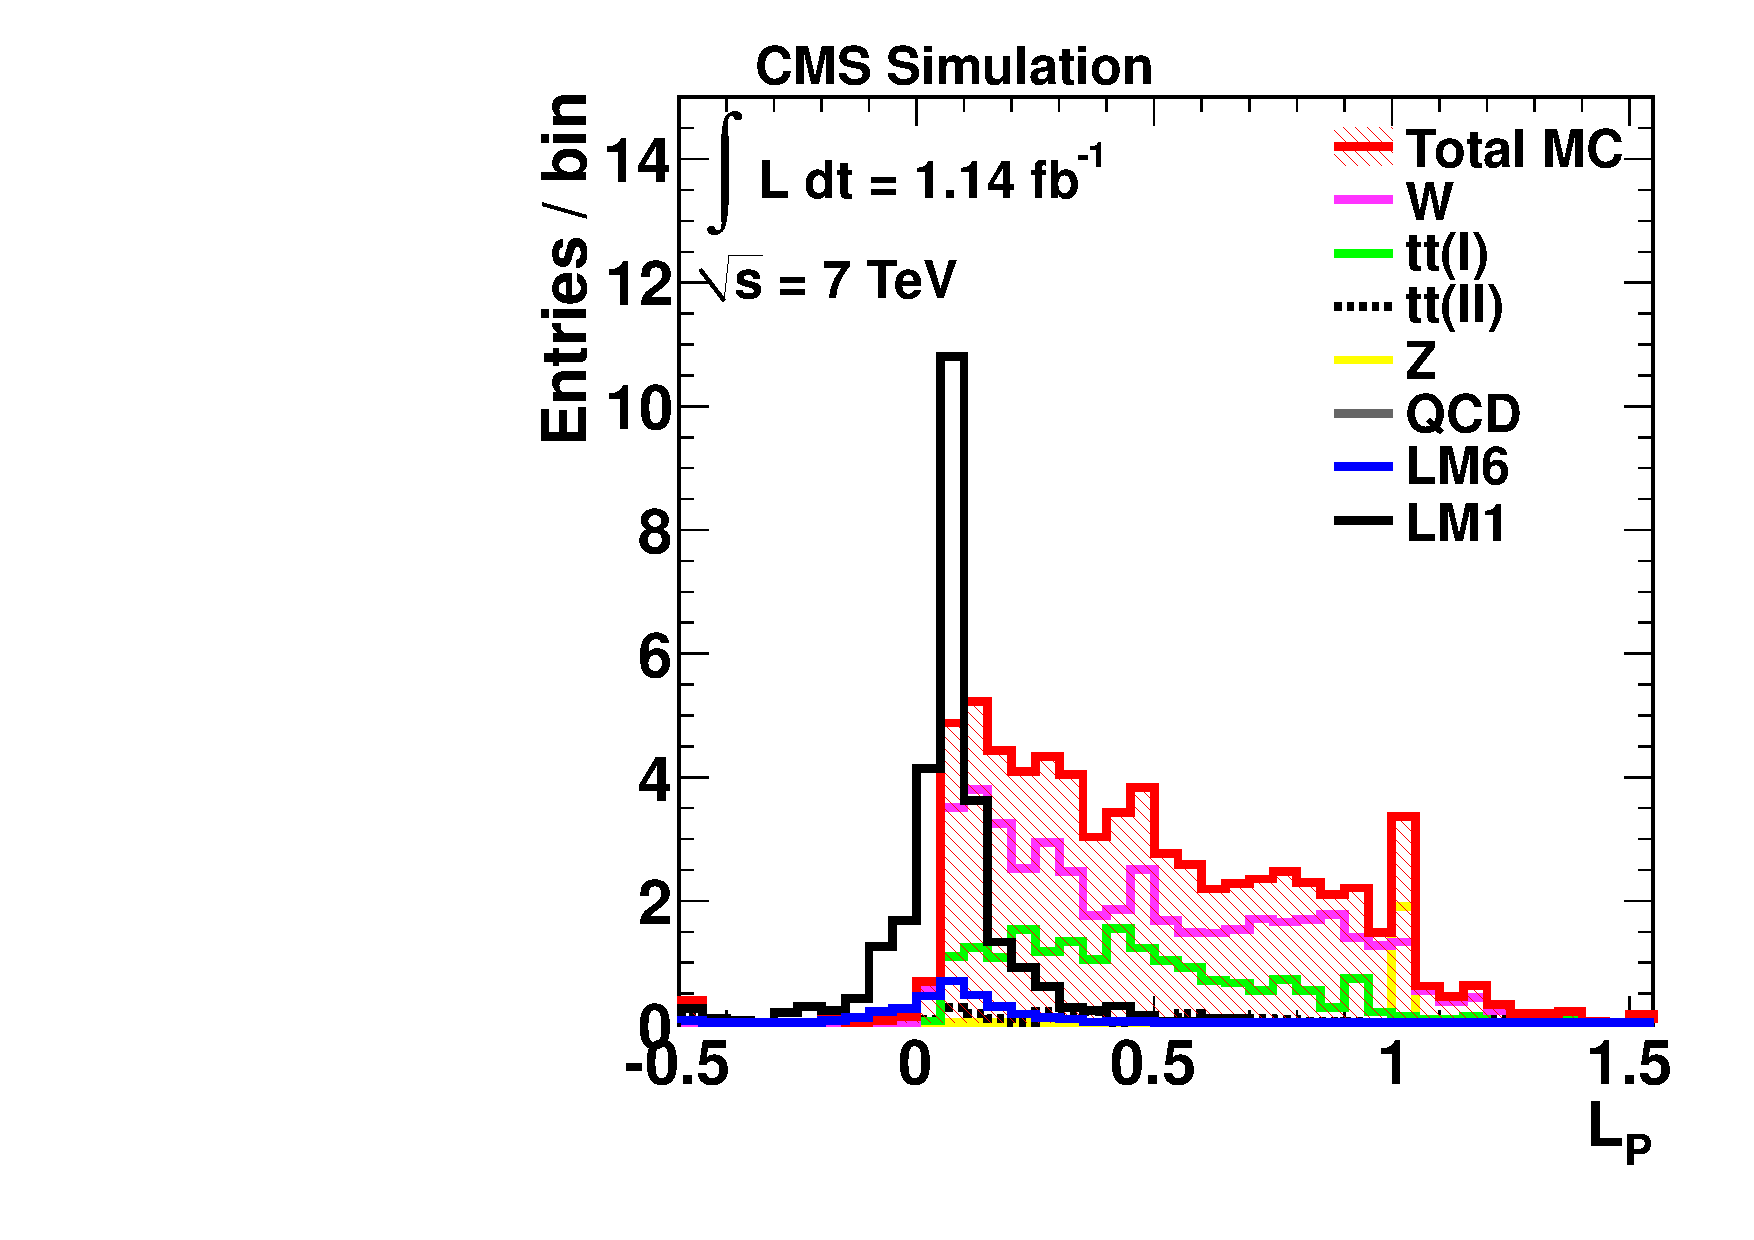
\includegraphics[width=0.3\textwidth]{fig/LP350_MCandSignal_Mu.pdf}}
\caption[]{}
\label{fig:susy_lp}
\end{figure}

In order to make use of the discrimination power afforded by the \LP shape, a
signal and control region are defined. The signal region is defined such that an
enriched sample of \ac{SUSY} events is obtained without being highly model
dependent. It should be stressed that the intent is not to eliminate the
background altogether in this region. The control region likewise must select a
sample of \ac{SM} background events with sufficient statistics whilst guarding
against excessive signal contamination from \ac{SUSY} models. By studying the
\LP distribution across the \ac{CMSSM} parameter space, \LPsignal for the signal
region and \LPcontrol for the control region were found to be suitable choices.

To predict the \ac{SM} background contamination in the \LPsignal region, a
translation factor, \RCS is calculated in simulation. This is defined as
\begin{equation}
\RCS = \frac{N^{\textrm{MC}}(\LPsignal)}{N^{\textrm{MC}}(\LPcontrol)}
\end{equation}
where $N^{\textrm{MC}}(\LPsignal)$ and $N^{\textrm{MC}}(\LPcontrol)$ represent
the population, as calculated in simulation of \ac{SM} events in the signal and
control regions respectively. Once calculated, \RCS may be used along with a
measurement of the control region in data to predict the \ac{SM} background
contribution present in the signal region,
\begin{equation}
N^{\textrm{data}}(\LPsignal) = \RCS N^{\textrm{data}}(\LPcontrol)
\end{equation}
Whilst in principle it is possible to perform a more, or even completely,
data-driven prediction by performing a template fit to the \LP shape in the
control region and extrapolating into the signal region, this strategy was
explored for some time and found to be frustrated by inadequate statistics, even
at relatively large integrated luminosities.

The advantage of the translation factor \RCS is that by taking the ratio from
simulation, there is significant cancellation of many systematic uncertainties,
including in particular the jet energy scale that proved to be significant for
the \PW polarisation analysis (see Section~\ref{sec:wpol_syst_jec}). Since these
uncertainties do not cancel completely, they will be full evaluated in
Section~\ref{sec:susy_systematics} and are included in the statistical treatment
described in Chapter~\ref{sec:interpretation}.

One last point concerning \RCS is that, so that the prediction is not dominated
by uncertainties stemming from limited statistics in the control region, a value
of $\RCS << 1$ is preferable. As we will see, relatively small values of \RCS
are obtained using the definitions given above.

\section{Object Definitions}
The basic object selection requirements were defined to be consistent between
several complementary leptonic \ac{SUSY} searches at \ac{CMS}. They are
described and motivated further in \cite{susy_selection_an}.

\subsection{Jets and Missing Energy}
Jets and missing energy quantities are taken from the particle flow algorithm,
as described in Section~\ref{sec:reco_pf}. In addition, jets are required to
pass the ``LOOSE'' selection criteria, namely
\begin{itemize}
\item At least two particles - at least one of them charged - in the jet.
\item Fraction of jet energy carried by neutral hadrons less than 99\%.
\item Charged and neutral electromagnetic fractions both less than 99\%.
\end{itemize}
All jets are required to have a transverse momentum, $\Pt > \unit{40}{\GeV}$ and
are required to be within the fiducial region of the tracker, $|\eta| <
2.4$. The total hadronic transverse energy, \HT is calculated from jets passing
this selection.

\subsection{Muons}
Muon reconstruction is described in Section~\ref{sec:reco_muons}. Global muons
are selected with a number of additional quality requirements. These are similar
to thoseused in the \PW polarisation analysis (see Section~\ref{sec:wpol_muons})
with certain adjustements made to ensure consistency with other analyses or
adapt to the different analysis requirements.
\begin{itemize}
\item A normalized $\chi^2 < 10$ on the global muon fit
\item More than 10 hits in the tracker (including at least 1 pixel hit) and
  $\geq 2$ matching segments in the muon chambers.
\item A transverse distance to the nominal interaction point, $d_0 <
  \unit{200}{\micro\metre}$ and longitudinal distance to the primary vertex $d_z
  < \unit{1}{\centi\metre}$
\item The uncertainty on the muon transverse momentum $\sigma(\Pt)/\Pt^2 <
  \unit{0.001}{\reciprocal\GeV}$
\item Each global muon must also qualify as a tracker muon.
\item A combined relative isolation (see Eqn~\ref{eqn:wpol_mu_comb_iso}) $\CombIso < 0.1$.
\end{itemize}

\textbf{Tight} muons are defined by the requirements given above. \textbf{Loose}
muons use an identical selection but with the \CombIso cut loosened to 0.15.

\subsection{Electrons}
\textbf{Tight} electrons are reconstructed as described in
Section~\ref{sec:reco_electrons} using the 80\% efficiency working point but
with impact parameter requirements identical to those used for the
muons. \textbf{Loose} electrons use the 95\% efficiency working point with the
impact parameter criteria loosened as for the muon case.

\subsection{Resolving Ambiguities}
Since the leptons used in this analysis use the traditional reconstruction
methods at \ac{CMS} while jets and \MET are taken from the \ac{PF} algorithm,
ambiguities can exist. In order to avoid double counting, these ambiguities are
resolved by several cleaning steps.

To remove jets dominated by a lepton, any jet found within a cone of 0.1 (0.3)
of a selected muon (electron) is removed from consideration. In addition, muons
within a cone of 0.3 of any jet are rejected.

A second step corrects the \MET for differences between \ac{PF} and global muon
reconstruction. Each global muon is matched to a corresponding \ac{PF} muon
within a cone of $\DeltaR < 0.1$. The absolute relative difference between the
transverse momenta is then calculated. For cases where no match is found or this
difference is $> 20\%$, the event is rejected. For cases where the difference is
smaller than 20\%, the \MET receives a vectorial collection.

\section{Analysis Selection}
Selection begins with a set of event cleaning cuts common to many analyses at
\ac{CMS}. These address known detector and reconstruction problems as well as
supressing machine backgrounds. They are fully detailed in
\cite{susy_selection_an}.

Lepton selection requires exactly one \textbf{Tight} electron or muon. To remove
dilepton events and minimise overlap with searches in multilepton final states,
events containing a second \textbf{Loose} lepton are vetoed.

After the initial lepton selection cuts, events can enter two independent
samples. The first is a control sample, inverting the jet multiplicity cut to
obtain a sample known to be overwhelmingly dominated by \ac{SM} backgrounds. To
compensate, this sample is selected with a slightly relaxed \HT cut. The second
sample was used for the actual analysis. A jet multiplicity cut, $\Njets \geq 3$
is applied as well as an \HT cut.

The data-driven control sample was used to test the analysis techniques before
they were applied in the search dataset. During this time, the search dataset
was not studied (or ``blinded'') to avoid changes in the analysis procedure that
might bias the result. Once the analysis method was fully refined, the search
sample was ``unblinded'' and major changes to the analysis were no longer
allowed.

Due to the unavailability of suitable efficient and unbiased triggers, the
control sample was considered only for the muon channel. For the electron
channel, validation work was performed instead in the $150 < \STlep <
\unit{250}{\GeV}$ bin. Trigger thresholds in the control sample necessitated
increasing the transverse momentum cut on the muon to \unit{35}{\GeV}.

The full cutflow is shown in Table~\ref{tbl:susy_cutflow}.

\ctable[
cap=\acs{SUSY} search selection requirements,
caption=Selection requirements for the \ac{SUSY} search in both the search
samples and the muon control sample. The lepton selection and veto requirements
are common to both samples.,
pos=h,
label=tbl:susy_cutflow
]{ll}{
}{\FL
Lepton Selection           & Exactly one \textbf{Tight} electron or muon \NN
                           & $|\eta^{\Pgm}| < 2.1$, $|\eta^{\Pe}| < 2.5$\NN
Lepton Veto                & Zero additional leptons passing \textbf{Loose} criteria\NN
                           & $P_T^{\Pgm} > \unit{15}{\GeV}$, $P_T^{\Pe} > \unit{20}{\GeV}$\NN
                           & $|\eta^{\Pgm}| < 2.5$, $|\eta^{\Pe}| < 2.5$\ML
Control Sample (\Pgm only) & $< 3$~jets \NN
                           & $P_T^{\Pgm} > \unit{35}{\GeV}$\NN
                           & $\HT > \unit{200}{\GeV}$ \ML
Analysis Sample            & $\geq 3$~jets \NN
                           & $P_T^{\Pl} > \unit{20}{\GeV}$\NN
                           & $\HT > \unit{500}{\GeV}$\LL
}

\subsection{Monte Carlo Expectations}
\ctable[
caption=Expected event yields in the signal region\, $\LP < 0.15$\, with
\unit{1.14}{\invfb} in the muon and electron channels.  The MC values are only
listed for illustration purposes.  The actual estimate of the number of SM
events in the signal region uses the method described in the text. The
contribution from QCD multijet production is expected to be negligible and is
thus not included in the table.,
pos=h!,
label=tbl:susy_mcexpectation_signal,
%doinside=\scriptsize
]{ccccccc}{
}{\FL
$\LP<0.15$          & \multicolumn{3}{c}{ Muons: \STlep range (GeV) } & \multicolumn{3}{c}{  Electrons: \STlep range (GeV) }\ML
Sample              & [250-350]                                         & [350-450]    & [450-$\inf$] & [250-350]   & [350-450]   & [450-$\inf$] \ML
\ttbar ($\ell$)     & 11.4$\pm$0.9                                      & 2.91$\pm$0.4 & 0.8$\pm$0.2  & 7.8$\pm$0.7 & 3.0$\pm$0.4 & 1.0$\pm$0.3\NN
\ttbar ($\ell\ell$) & 2.2$\pm$0.4                                       & 0.6$\pm$0.2  & 0.1$\pm$0.1
                    & 2.4$\pm$0.4                                       & 0.7$\pm$0.2  & 0.4$\pm$0.2\NN
W                   & 14.5$\pm$0.6                                      & 8.0$\pm$0.5  & 5.6$\pm$0.4
                    & 10.5$\pm$0.5                                      & 5.2$\pm$0.4  & 4.7$\pm$0.3\NN
Z                   & 0$\pm$1.5                                         & 0$\pm$1.5    & 0$\pm$1.5
                    & 0$\pm$1.5                                         & 0$\pm$1.5    & 0$\pm$1.5\NN
Total MC            & 28.1$\pm$1.1                                      & 11.5$\pm$0.7 & 6.5$\pm$0.4
                    & 20.8$\pm$1.0                                      & 8.8$\pm$0.6  & 6.1$\pm$0.5\NN
LM1                 & 24.2$\pm$0.9                                      & 23.1$\pm$0.9 & 16.2$\pm$0.7
                    & 22.9$\pm$0.9                                      & 20.8$\pm$0.8 & 14.7$\pm$0.7\NN
LM3                 & 24.8$\pm$0.8                                      & 16.7$\pm$0.6 & 9.7$\pm$0.5
                    & 22.8$\pm$0.7                                      & 14.8$\pm$0.6 & 9.7$\pm$0.5\NN
LM6                 & 1.9$\pm$0.0                                       & 2.5$\pm$0.1  & 5.9$\pm$0.1
                    & 1.7$\pm$0.0                                       & 2.3$\pm$0.1  & 5.3$\pm$0.1 \LL
}
\ctable[
caption=Expected event yields in the control region\, $\LP > 0.30$\, with
\unit{1.14}{\invfb} in the muon and electron channels.  The MC values are only
listed for illustration purposes.  The actual estimate of the number of SM
events in the signal region uses the method described in the text.,
pos=h!,
label=tbl:susy_mcexp_control,
%doinside=\scriptsize
]{ccccccc}{
}{\FL
$\LP>0.30$          & \multicolumn{3}{c}{  Muons: \STlep range (GeV) } & \multicolumn{3}{c}{  Electrons: \STlep range (GeV) } \ML
Sample              & [250-350]                                        & [350-450]    & [450-$\inf$] & [250-350] & [350-450] & [450-$\inf$] \ML
\ttbar ($\ell$)     & 43.4$\pm$1.7                                     & 12.3$\pm$0.9 & 2.7$\pm$0.4
                    & 42.2$\pm$1.7                                     & 11.4$\pm$0.8 & 2.9$\pm$0.4\NN
\ttbar ($\ell\ell$) & 5.2$\pm$0.6                                      & 1.6$\pm$0.3  & 0.4$\pm$0.2
                    & 2.5$\pm$0.4                                      & 1.4$\pm$0.3  & 0.3$\pm$0.1\NN
W                   & 67.1$\pm$1.3                                     & 27.5$\pm$0.8 & 15.3$\pm$0.6
                    & 57.5$\pm$1.2                                     & 24.3$\pm$0.8 & 14.7$\pm$0.6\NN
Z                   & 0$\pm$1.5                                        & 1.7$\pm$1.5  & 0$\pm$1.5
                    & 7.5$\pm$3.6                                      & 0$\pm$0      & 0$\pm$0\NN
QCD                 & 0$\pm$1.5                                        & 0$\pm$1.5    & 0$\pm$1.5
                    & 10.4$\pm$3.0                                     & 7.2$\pm$1.7  & 3.8$\pm$0.7\NN
Total MC            & 116$\pm$2                                        & 43.4$\pm$2.3 & 18.4$\pm$0.8
                    & 120$\pm$5                                        & 44.3$\pm$2.1 & 21.7$\pm$1.1\NN
LM1                 & 2.8$\pm$0.3                                      & 1.4$\pm$0.2  & 0.8$\pm$0.2
                    & 2.9$\pm$0.3                                      & 2.0$\pm$0.3  & 1.3$\pm$0.2\NN
LM3                 & 9.7$\pm$0.5                                      & 4.2$\pm$0.3  & 2.3$\pm$0.2
                    & 9.1$\pm$0.5                                      & 4.2$\pm$0.3  & 2.5$\pm$0.2\NN
LM6                 & 0.5$\pm$0.0                                      & 0.4$\pm$0.0  & 0.9$\pm$0.0
                    & 0.5$\pm$0.0                                      & 0.4 $\pm$0.0 & 0.9$\pm$0.0\LL
}

\section{Triggers and Datasets}
Due to the construction of \STlep, events may be selected with moderate \MET
(and a high \Pt lepton) or large \MET (and a modertate \Pt lepton). This
necessitates a different trigger strategy to that used in other leptonic
\ac{SUSY} searches at \ac{CMS} which typically only select high \MET events.

For the search sample, a set of single-lepton cross-triggers are used, selecting
events with a single lepton in association with a large amount of hadronic
activity, \HT. As the luminosity increased during the 2011 run, it was necessary
to introduce a third requirement: a moderate cut on the \MET. The full list of
triggers used for both lepton channels are shown in
Table~\ref{tbl:susy_triggers}

\ctable[
cap=Triggers used in the \ac{SUSY} search analysis,
caption=Triggers used in the \ac{SUSY} search analysis for muon and electron search samples and the muon control sample,
pos=h!,
label=tbl:susy_triggers,
doinside=\scriptsize
]{ll}{
}{\FL
\multicolumn{2}{c}{\textbf{Search Sample}}\ML
\Pgm & HLT\_Mu8\_HT200\_v* \NN
     & HLT\_Mu15\_HT200\_v* \NN
     & HLT\_Mu15\_HT250\_PFMHT20\_v* \ML
\Pe  & HLT\_Ele10\_CaloIdL\_CaloIsoVL\_TrkIdVL\_TrkIsoVL\_HT200\_v* \NN
     & HLT\_Ele15\_CaloIdT\_CaloIsoVL\_TrkIdT\_TrkIsoVL\_HT250\_v* \NN
     & HLT\_HT250\_Ele5\_CaloIdVL\_TrkIdVL\_CaloIsoVL\_TrkIsoVL\_PFMHT35\_v* \NN
     & HLT\_HT300\_Ele5\_CaloIdVL\_TrkIdVL\_CaloIsoVL\_TrkIsoVL\_PFMHT40\_v* \ML
\multicolumn{2}{c}{\textbf{Control sample}}\ML
\Pgm & HLT\_Mu20\_v*, HLT\_IsoMu17\_v*\NN
     & HLT\_Mu30\_v*, HLT\_IsoMu24\_v*\LL
}

All signal and background Monte Carlo samples are from the Summer11 \ac{CMS}
\unit{7}{\TeV} production using \ac{CMSSW} 42. All processes are simulated using
the Madgraph matrix element generator, with the exception of the \ac{QCD} and
\ac{SUSY} signal samples which use \ac{PYTHIA} 6. All datasets, with the
exception of the \ac{SUSY} signal scan used to derive the limit use the full
detector simulation. The \ac{SUSY} signal scan uses the \ac{FASTSIM} simplified
simulation package to reduce processing time. All samples contain data-like
pile-up conditions, with a reweighting procedure used througout to reflect the
exact vertex multiplicity distribution in the data.

In addition to the standard \Wjets sample, an enriched sample with a
generator-level $\HT > \unit{300}{\GeV}$ cut. This increases the available
statistics, minimising the statistical error on \RCS.

\section{Control Region}
In order to test that the simulation of electroweak background processes can be
relied upon for the calculation of the translation factor \RCS, the procedure is
first performed in the control sample. With jet multiplicity cut inverted, it is
not expected for new physics to appear significantly in this sample. It is
expected therefore that the background prediction in the signal region should
agree well with the observed signal yield. Furthermore, the level of agreement
between data and simulation is also important in establishing the method.

A summary of the yields in the \LPcontrol and \LPsignal regions in the control
sample is given in Table~\ref{tbl:susy_control_yields}. Shown are the yields per
subprocess from simulation - used to calculate the factor \RCS, the yields in
data and the resulting background prediction. Comparing the background
prediction, it is seen to agree within errors with the observe number of events
in the signal region. The uncertainties stem from the limited data statistics of
the control region and the limited Monte Carlo statistics used in the
calculation of \RCS.

\ctable[
caption=SUSY Control Yields,
pos=h!,
label=tbl:susy_control_yields,
%doinside=\scriptsize
]{ccccccc}{
}{\FL
 & \multicolumn{3}{c}{Control Region: \LPcontrol} & \multicolumn{3}{c}{Signal Region: \LPsignal} \ML
Sample      & [250-350]    & [350-450]    & [450-$\inf$] & [250-350]             & [350-450]            & [450-$\inf$]\ML
\ttbar      & 50.1$\pm$1.8 & 7.8$\pm$0.7  & 2.8$\pm$0.4  & 10.5$\pm$0.8          & 2.8$\pm$0.4          & 0.7$\pm$0.2 \NN
W           & 959$\pm$24   & 162$\pm$9.7  & 46.2$\pm$5.2 & 83.7$\pm$7.0          & 22.8$\pm$3.7         & 12.3$\pm$2.8 \NN
Z           & 45.3$\pm$9.2 & 4.7$\pm$2.9  & 3.9$\pm$2.8  & 1.8$\pm$1.8           & 0$\pm$1.8            & 0$\pm$1.8 \NN
QCD         & 2.7$\pm$1.7  & 0.8$\pm$0.8  & 0$\pm$0.8    & 0$\pm$1.4             & 0$\pm$1.3            & 0$\pm$1.3 \NN
Total MC    & 1054$\pm$26  & 174$\pm$10.2 & 52.9$\pm$5.9 & 96$\pm$7.3            & 25.6$\pm$3.7         & 13$\pm$2.8 \NN
data        & 1051         & 179          & 52           & 92                    & 24                   & 11 \NN
SM Estimate &              &              &              & 95.8$\pm$10.2$\pm$7.6 & 26.3$\pm$5.5$\pm$4.1 & 12.8$\pm$4.0$\pm$3.0\NN
LM6         & 0.3$\pm$0.0  & 0.2$\pm$0.0  & 0.4$\pm$0.0  & 1.0$\pm$0.0           & 1.0$\pm$0.0          & 2.4$\pm$0.1 \LL
}


Comparisons of the variables \STlep, \MT and \Ptmu between data and simulation
are shown in Figure~\ref{fig:susy_mucontrol_kin}. A similar comparison is shown
for the \LP variable in bins of \STlep in
Figure~\ref{fig:susy_mucontrol_lp}. These distributions are those used to derive
the numbers shown in Table~\ref{tbl:susy_control_yields}. The data is seen to be
adequately described by the simulation.
\begin{figure}
\centering
\subfloat[]{\label{fig:susy_mucontrol_st}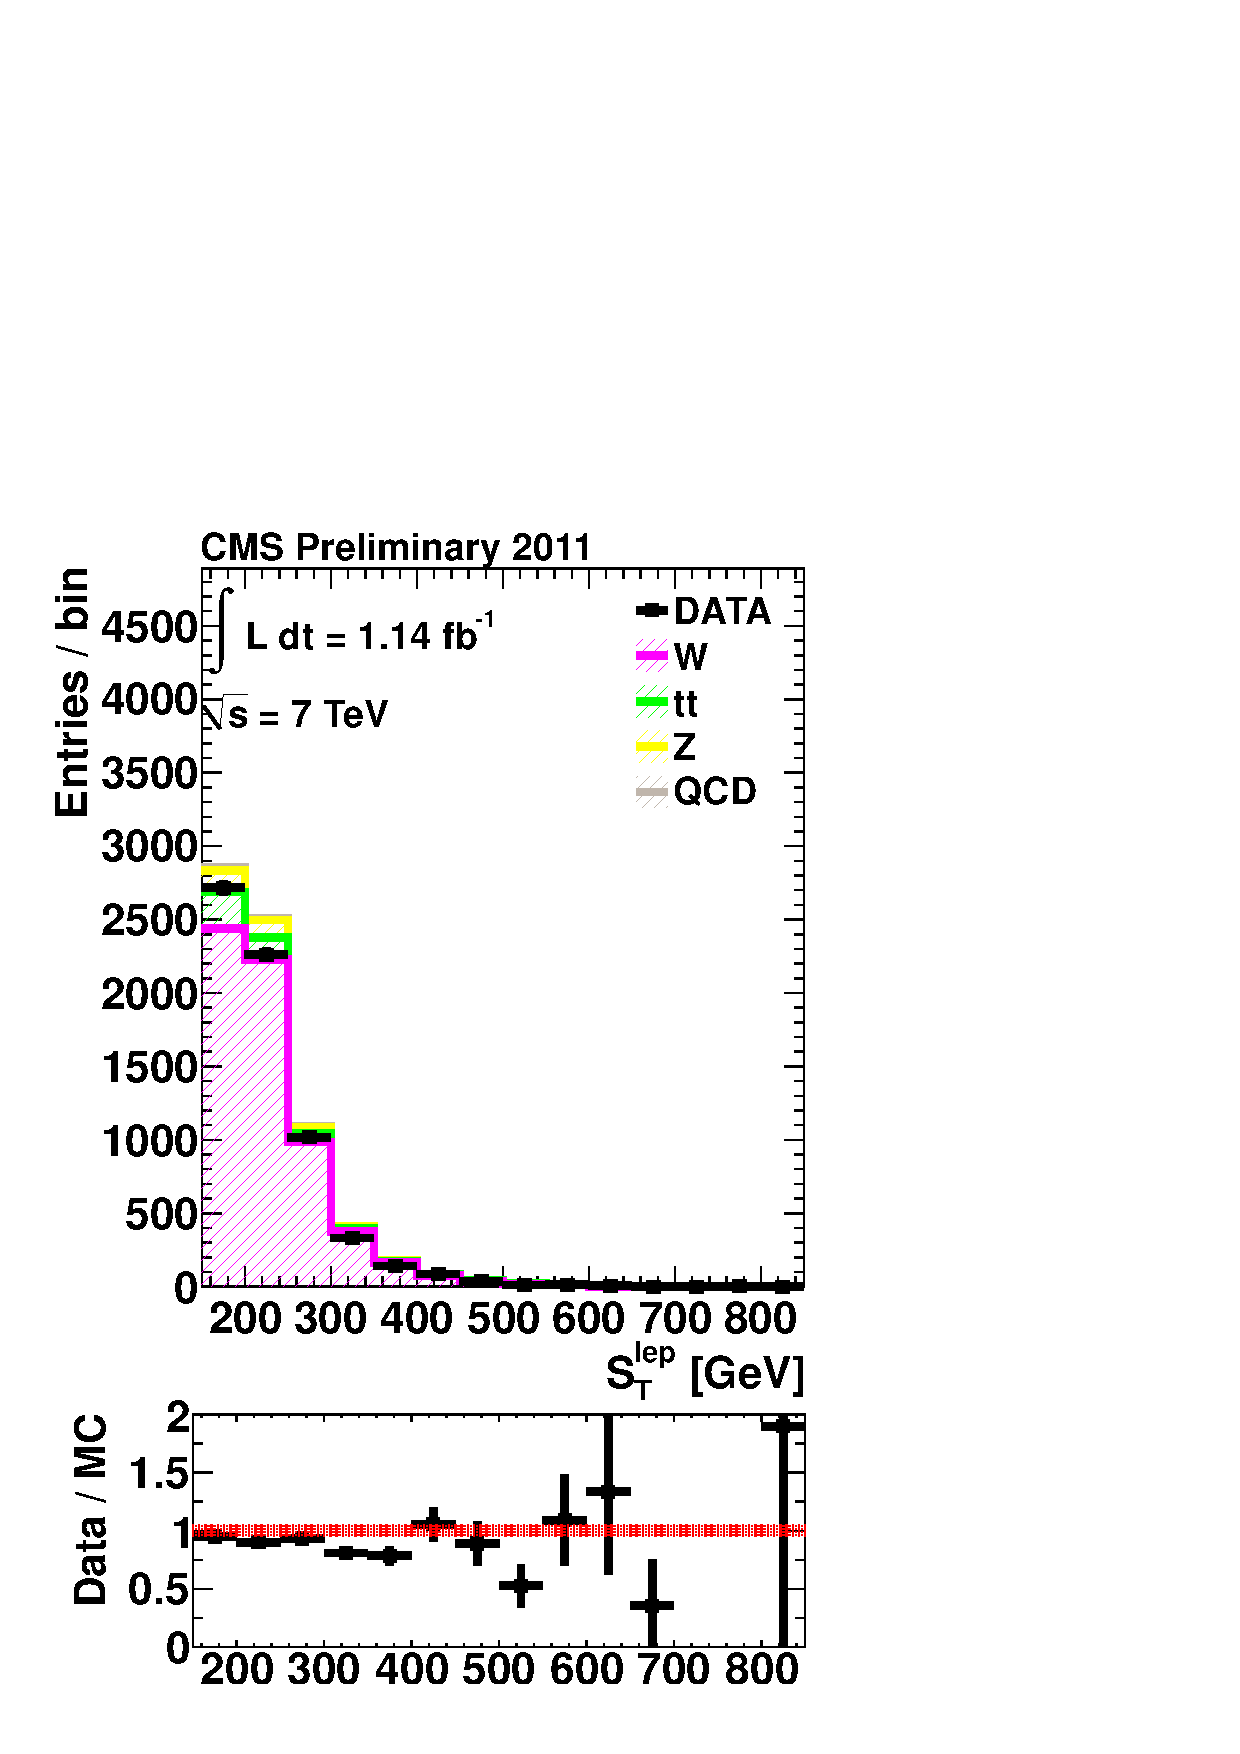
\includegraphics[width=0.3\textwidth]{fig/MuControl_ST150toInf}}\quad
\subfloat[]{\label{fig:susy_mucontrol_mt}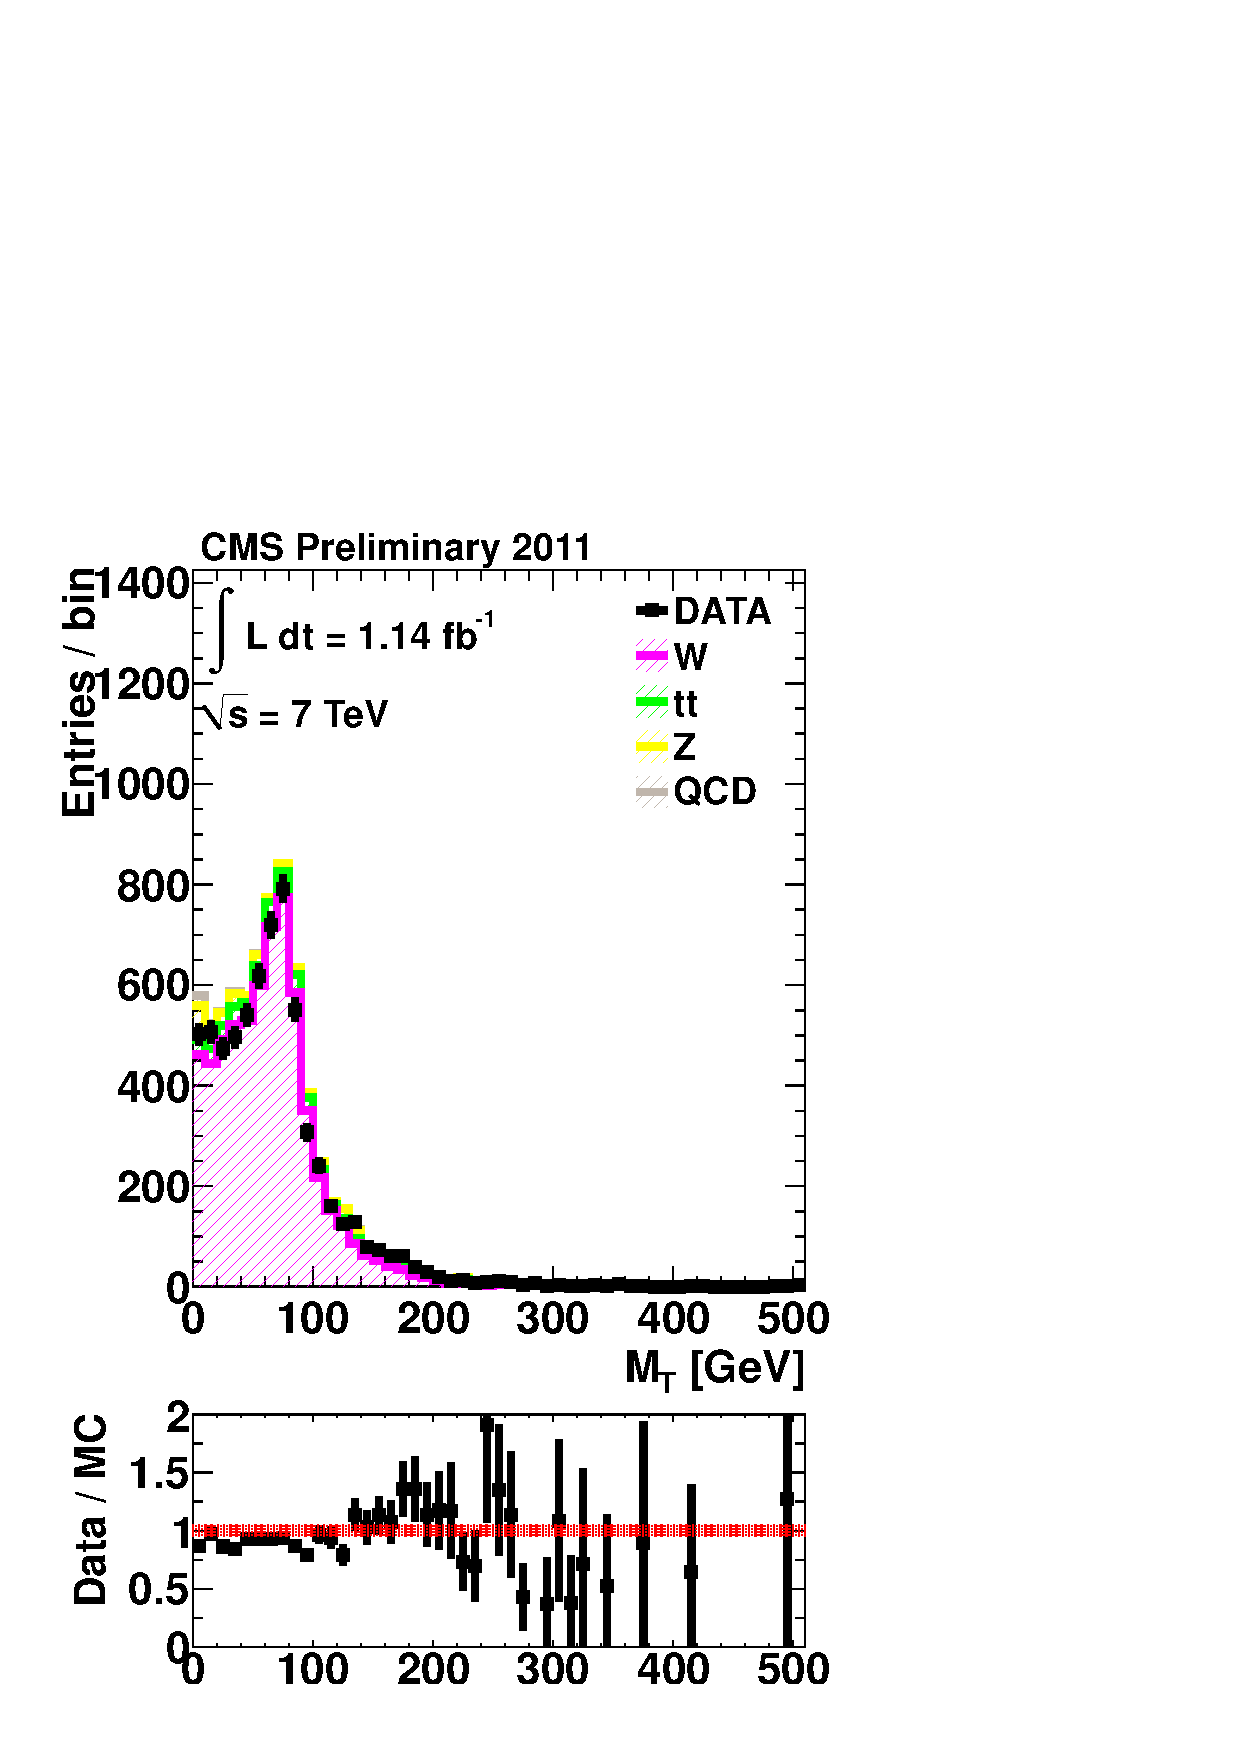
\includegraphics[width=0.3\textwidth]{fig/MuControl_MT150toInf}}\quad
\subfloat[]{\label{fig:susy_mucontrol_pt}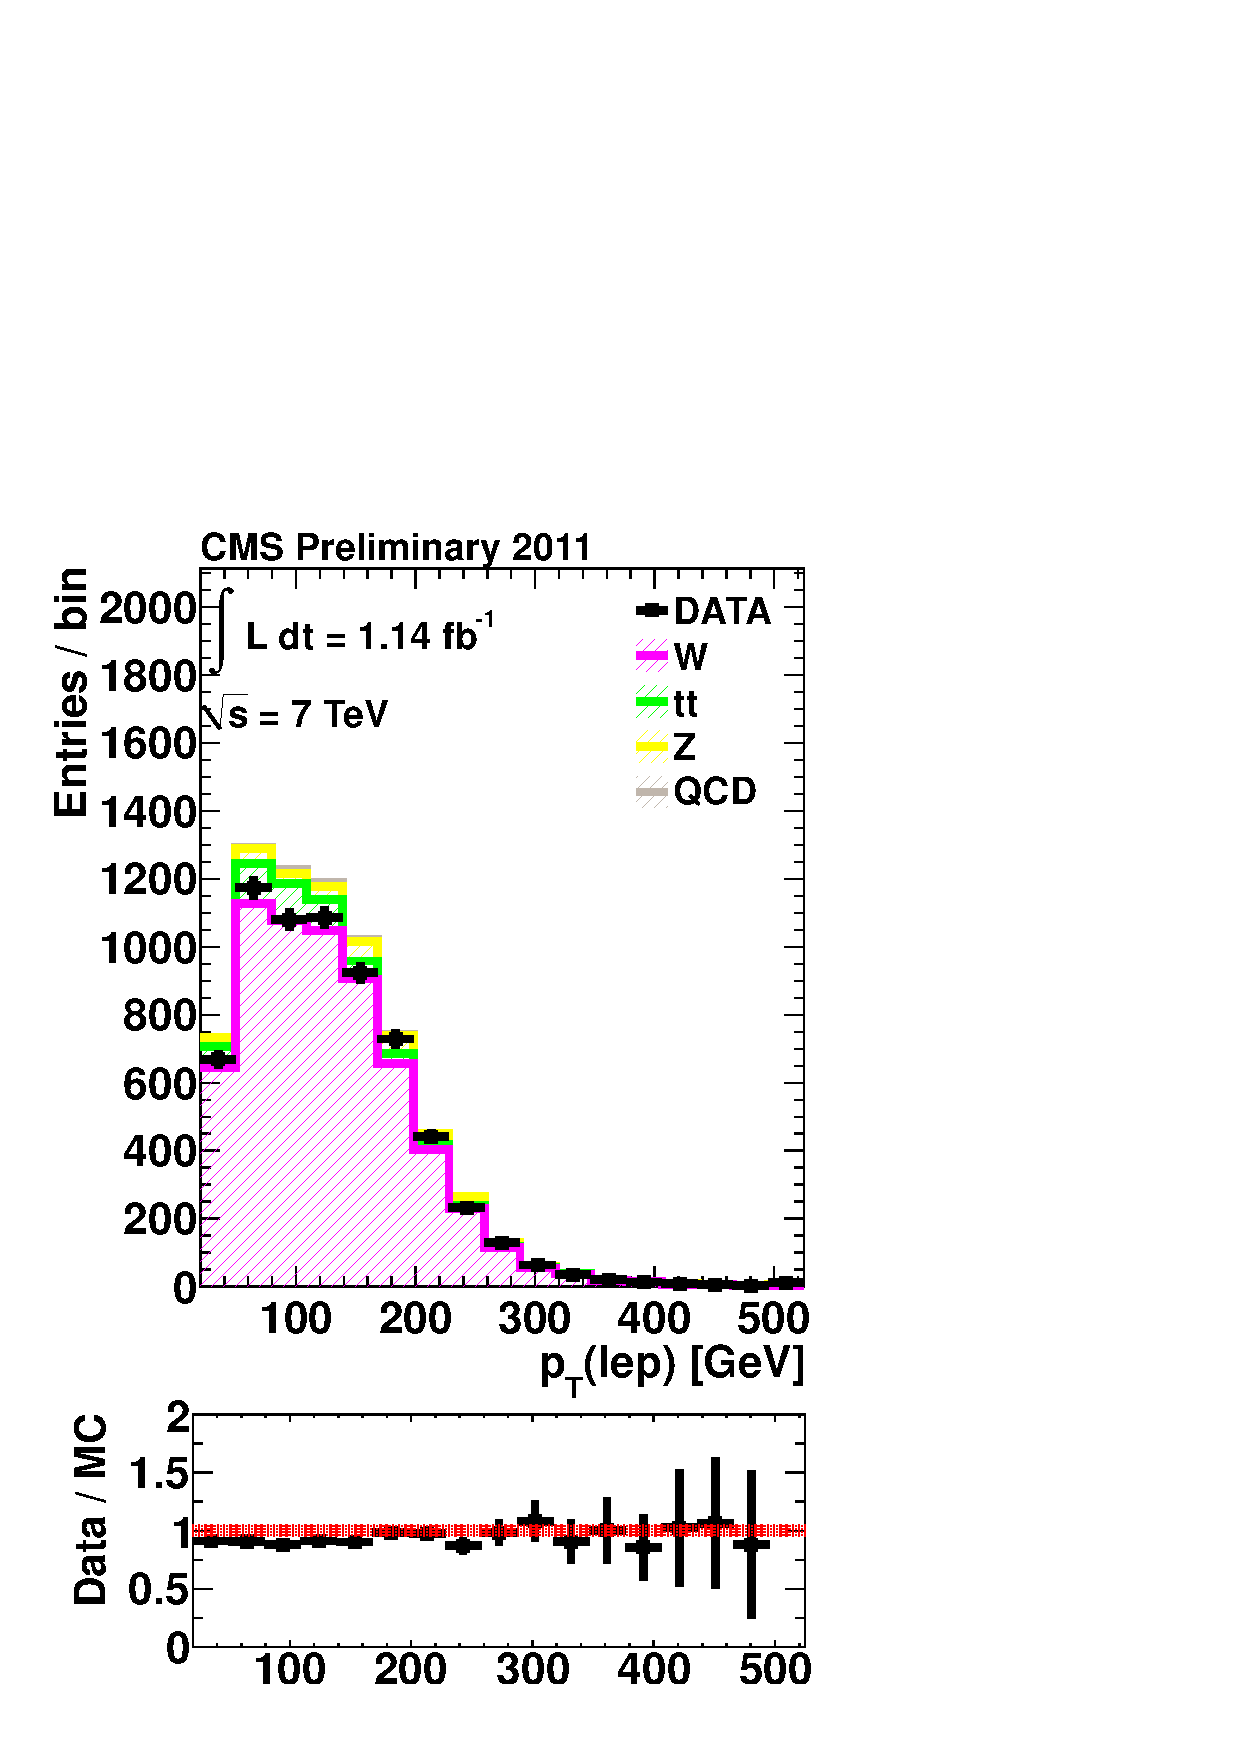
\includegraphics[width=0.3\textwidth]{fig/MuControl_MuPt150toInf}}
\caption[]{}
\label{fig:susy_mucontrol_kin}
\end{figure}

\begin{figure}
\centering
\subfloat[]{\label{fig:susy_mucontrol_lp250}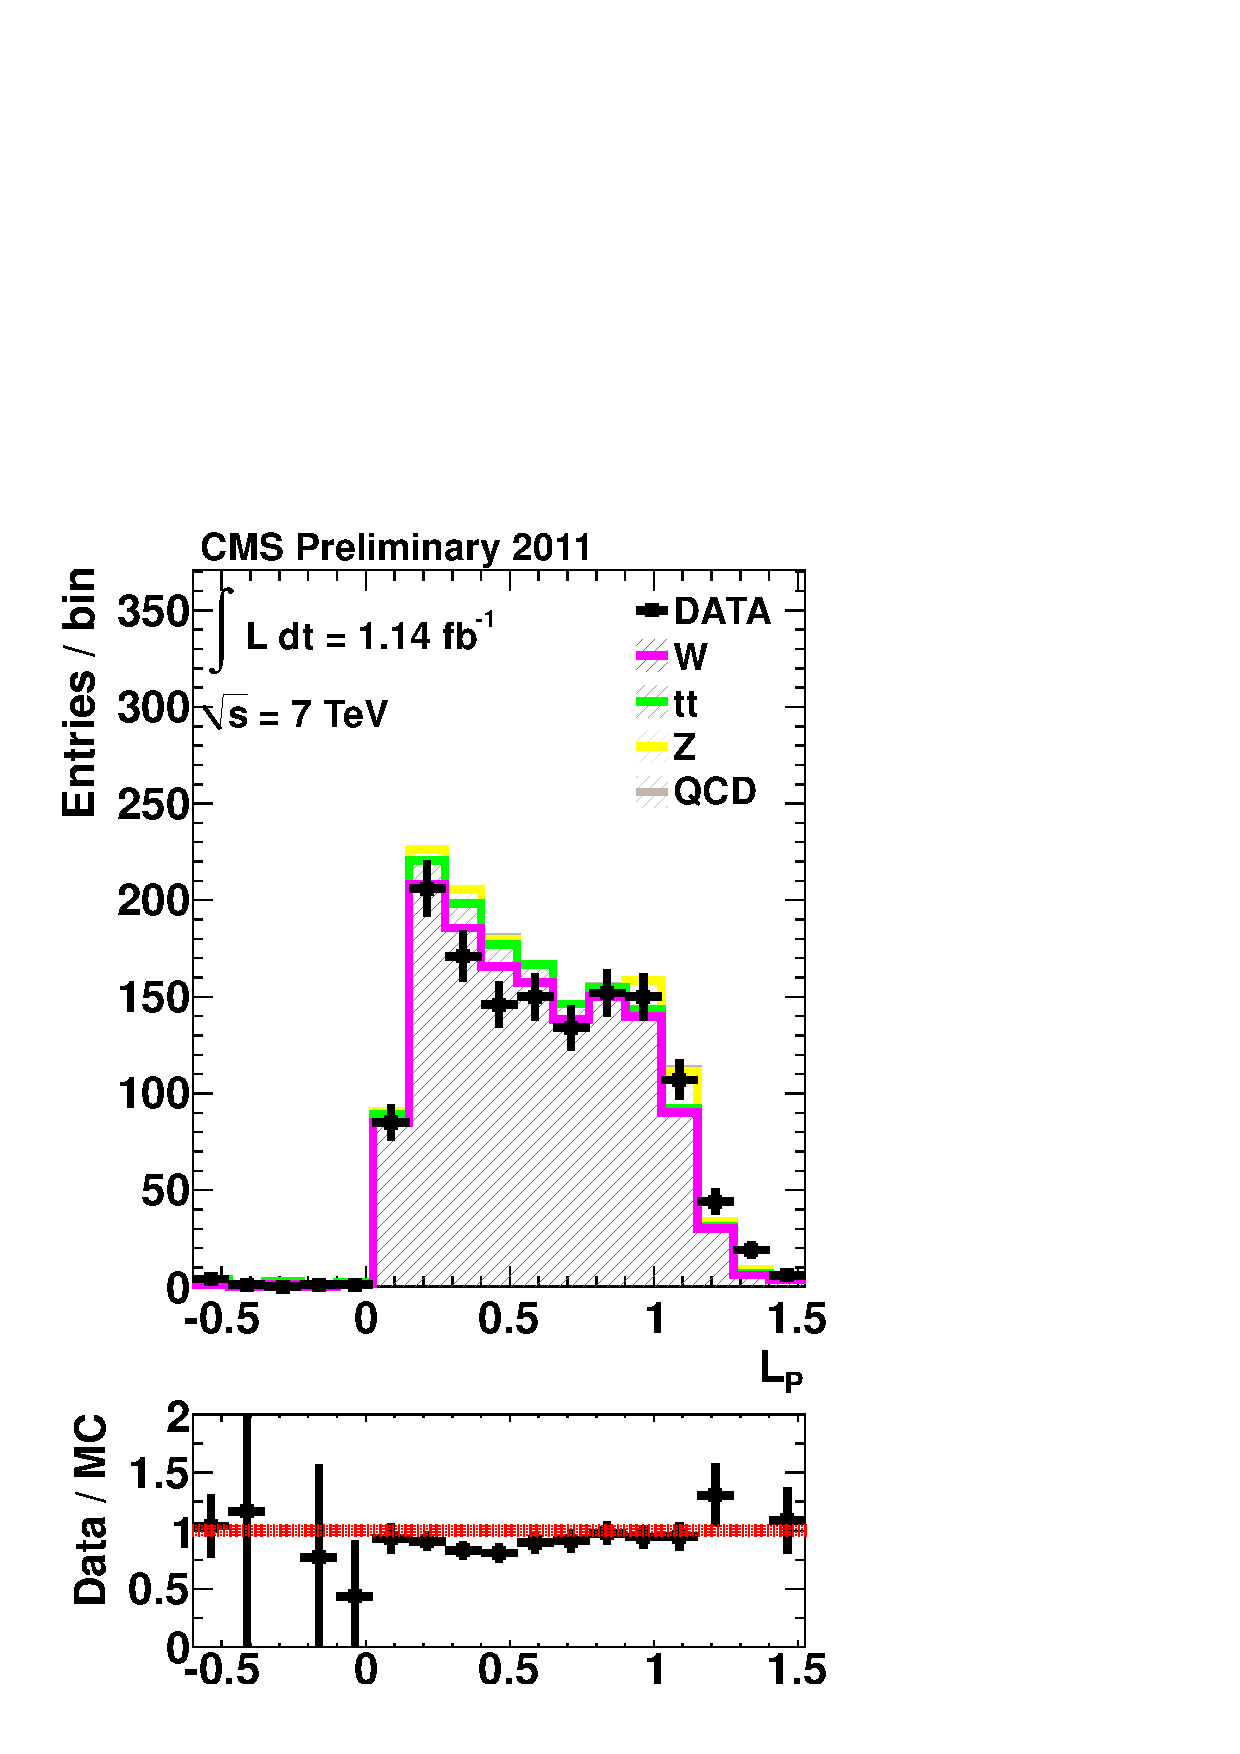
\includegraphics[width=0.3\textwidth]{fig/MuControl_LP250}}\quad
\subfloat[]{\label{fig:susy_mucontrol_lp350}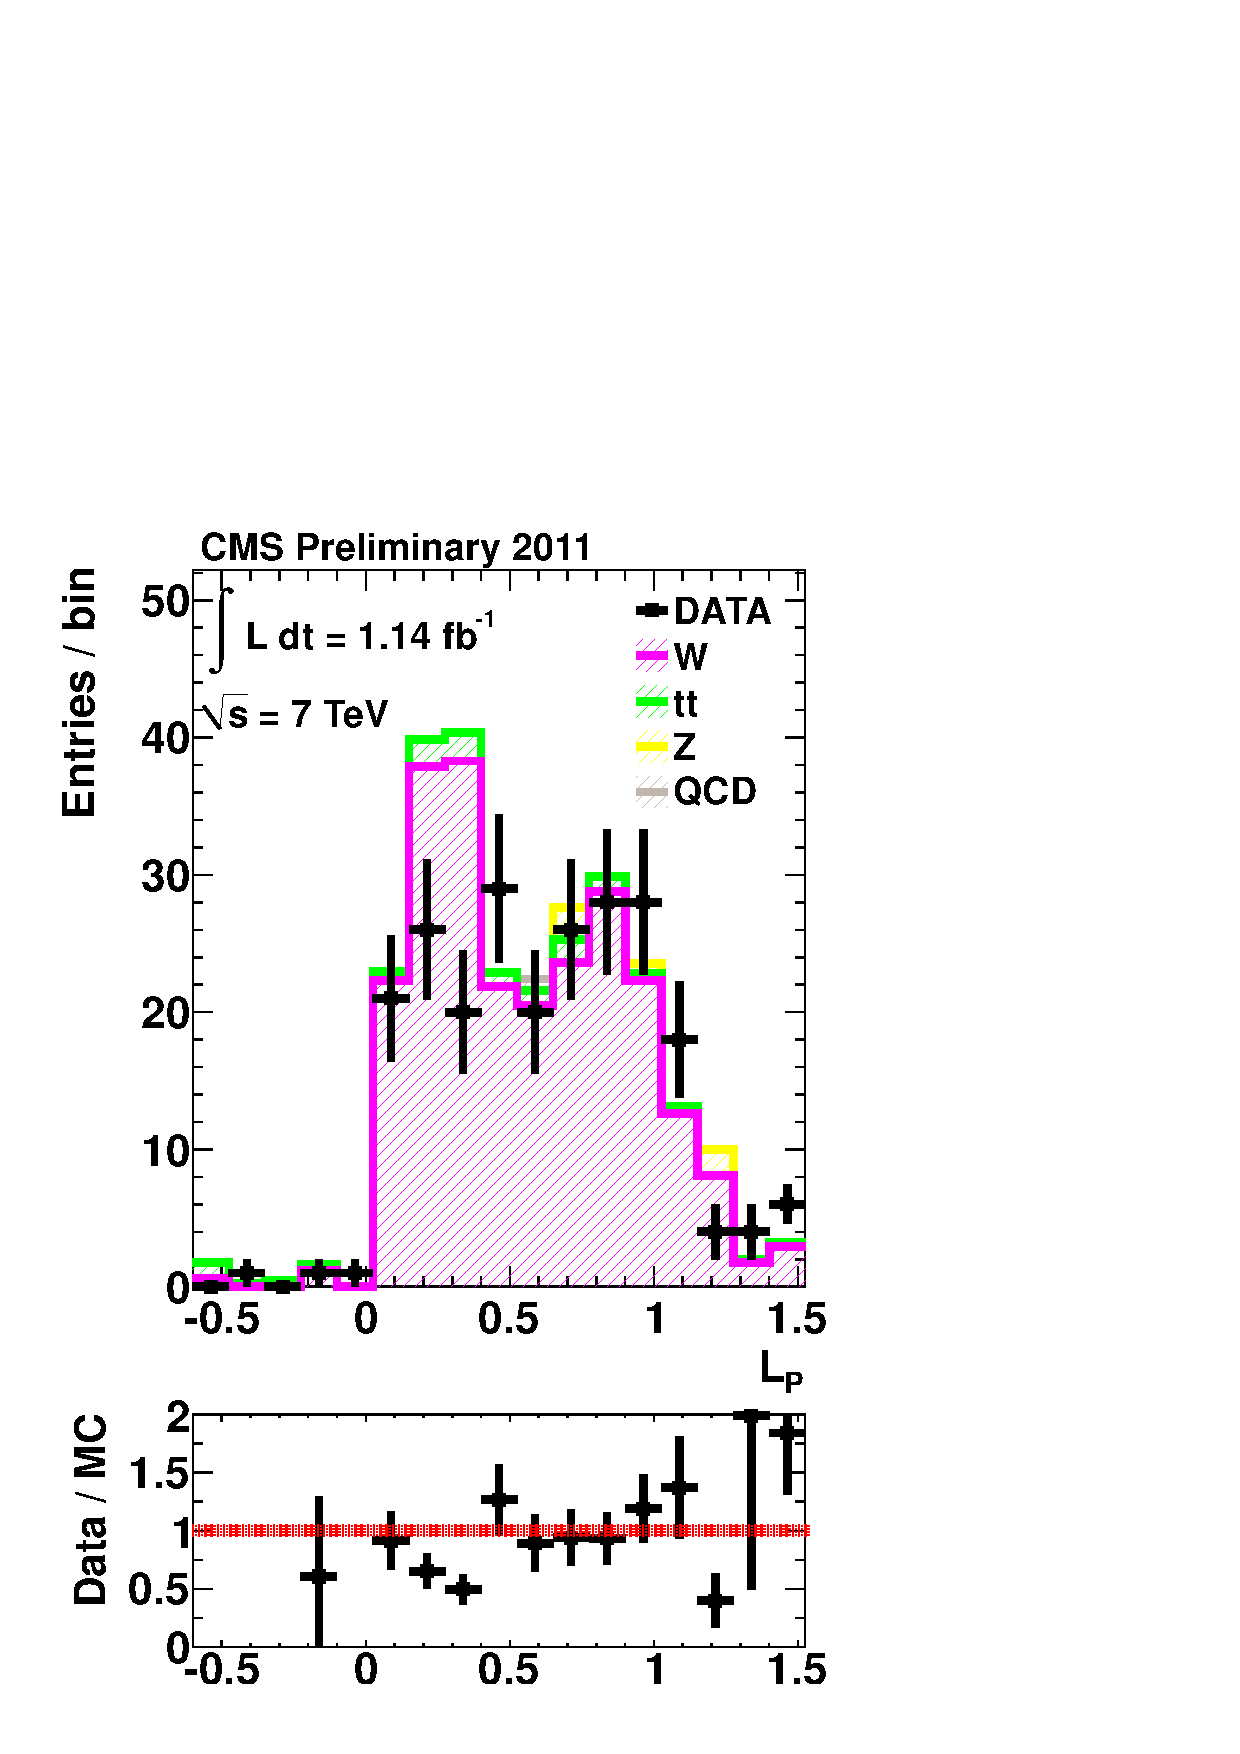
\includegraphics[width=0.3\textwidth]{fig/MuControl_LP350}}\quad
\subfloat[]{\label{fig:susy_mucontrol_lp450}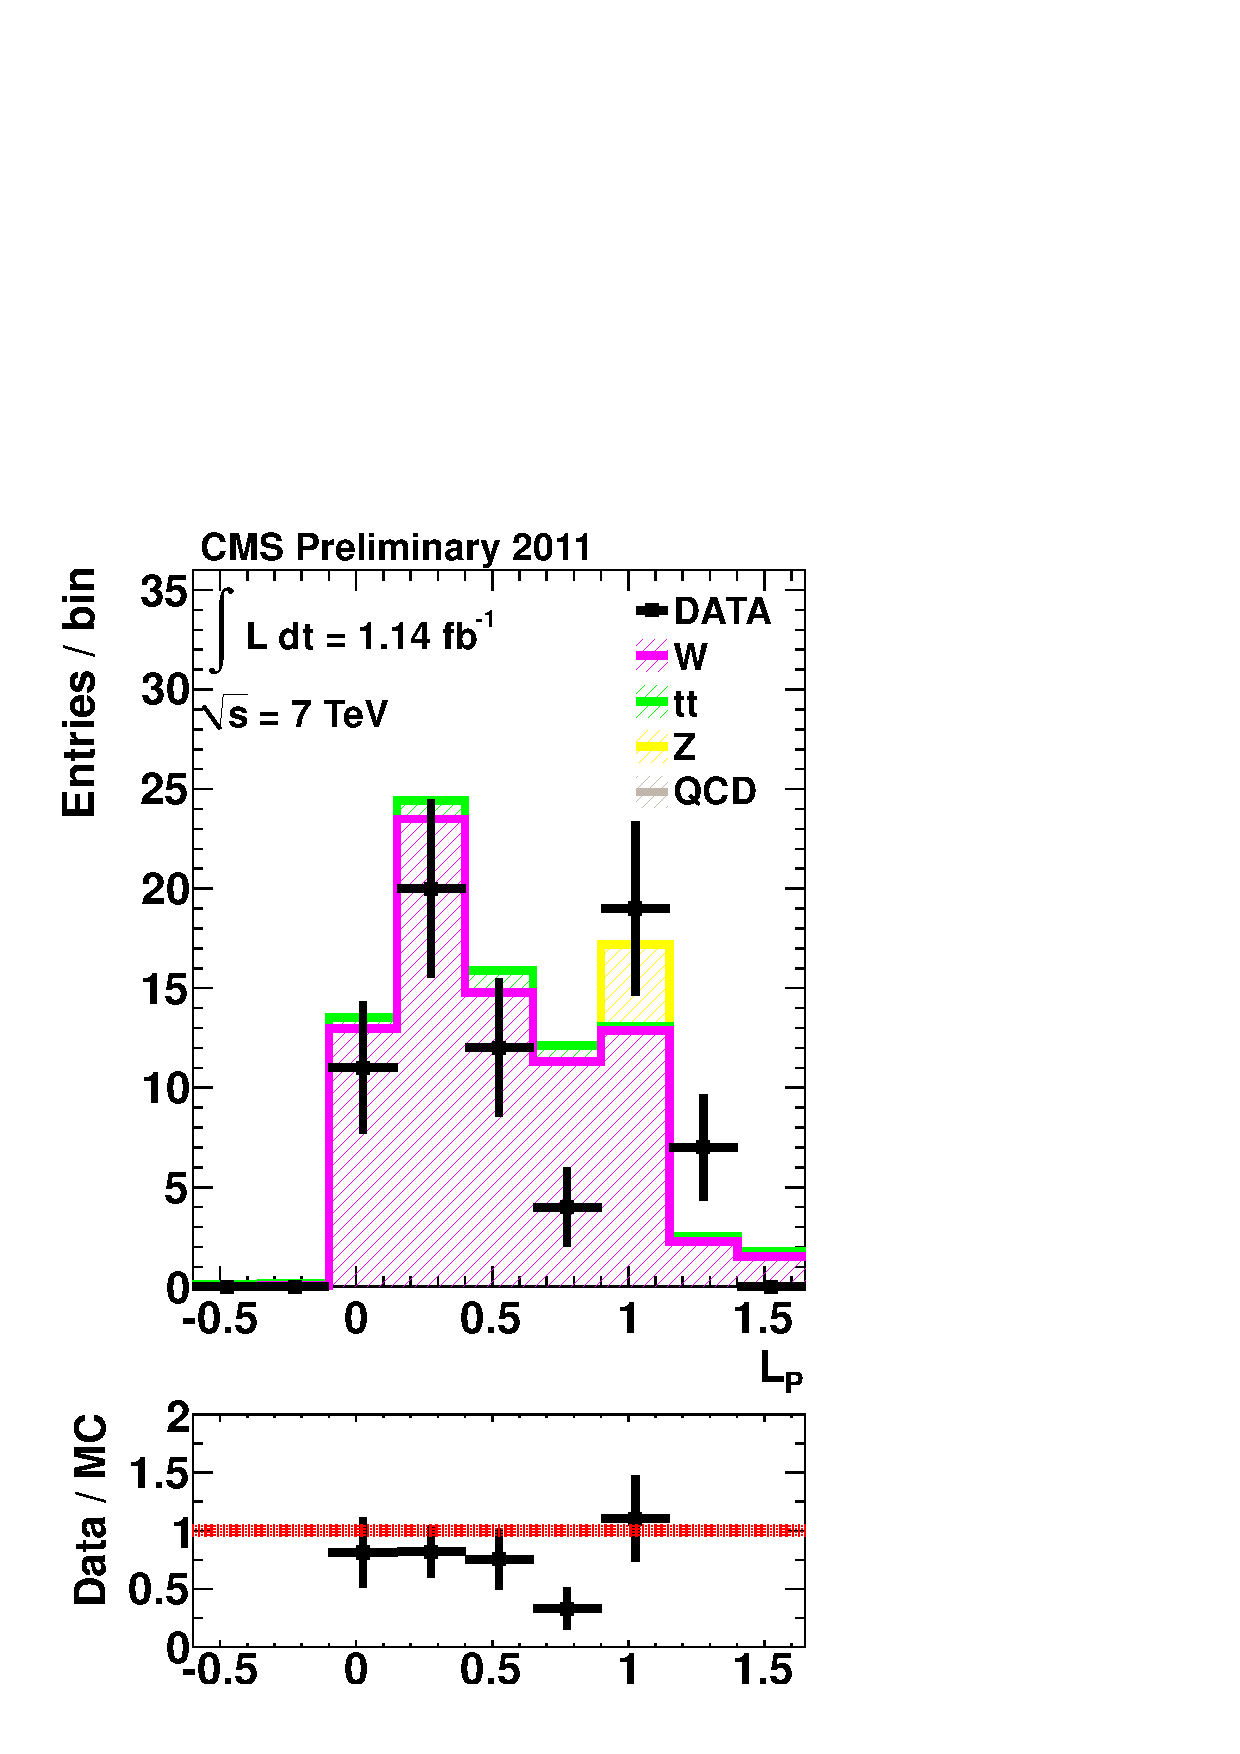
\includegraphics[width=0.3\textwidth]{fig/MuControl_LP450}}
\caption[]{}
\label{fig:susy_mucontrol_lp}
\end{figure}

\section{Background Prediction}
As for the \PW polarisation analysis, the background from \ac{QCD} multijet
events again presents a difficulty. In the muon channel, the \ac{QCD}
contribution is once again small to negligible as evidenced in
Table~\ref{tbl:susy_mcexp_control}. For this, it is sufficient to calculate
only an upper bound. For the electron channel, as before, the contribution is
much larger. Fortunately, the methods outlined in
Section~\ref{sec:wpol_data_driven_bg} prove to be effective again, with some
adaptation.

\subsection{Muons}
A conservative upper limit on the \ac{QCD} background in the muon channel is
obtained from a data-driven control sample by inverting the isolation cut, $0.2
< \CombIso < 0.5$. In order to further enrich \ac{QCD} events whilst supressing
electroweak backgrounds in this sample, a $\MET < \unit{20}{\GeV}$ cut is also
applied. Even with these cuts, significant electroweak contamination
remains. The significance of the vertex impact paramter is used as an additional
handle by requiring $\sigma(D_0) > 3$. The ratio $N(\CombIso < 0.1/N(0.2 <
\CombIso < 0.5)$ in this sample is then used to derive an upper limit on the
\ac{QCD} contribution. This limit is conservative given that electroweak
background are present in the ratio. It is seen in Table~TODO that the \ac{QCD}
background is negligible in all \STlep bins and is ignored in the subsequent
analysis.

\subsection{Electrons}
\label{sec:susy_electron_bgpredict}
In the case of the electrons, a strategy similar to that used in the \PW
polarisation analysis is employed. As before, the electron identification
variables \deltaetain and \deltaphiin are inverted. In addition, to ensure
adequate statistics the \D0 and \Dz cuts are removed and the isolation cut is
relaxed. The \D0 and \Dz cuts were not present in the \PW polarisation
selection. Although the present analysis benefits from a dataset $\sim 30$ times
larger than that used for the previous measurement, statistics are hurt by the
generally tighter kinematic cuts.

In addition, it was observed during studies for the \PW polarisation measurement
that the shape of the QCD template was affects by a cut on \PtW. Thus it should
be assumed to depend too on \STlep, necessitating the use of independent
templates for each \STlep bin. A comparison of the selected and anti-selected
shapes in simulated \ac{QCD} events is shown in Figure~\ref{fig:susy_elqcd_selasel}. This may be
compared with those derived in the \PW polarisation analysis (see
Figure~\ref{fig:wpol_ele_sel_antisel}). Differences may be accounted for by the
modified electron selection and kinematic cuts.

As in the \PW polarisation analysis, a binned maximum likelihood fit is
performed using electroweak background templates for the electroweak backgrounds
derived from simulation. To avoid the potential effects of signal contamination,
the fit region is restricted to \LPcontrol and then the fit result is used to
extrapolate into \LPsignal. The results of these fits are shown in
Figures~\ref{fig:susy_elqcd_fitresult150}
and~\ref{fig:susy_elqcd_fitresult250}. The predictions of the \ac{QCD} and
electroweak background contamination can be seen in Table~TODO. The \ac{QCD}
contamination in the signal region is seen to be negligible.

The results of the fit can be used to directly predict the background
contamination in the signal region. However, in order to compare systematic
uncertainties with the muon channel, a corrected \RCS is calculated from the fit
results. The systematic uncertainties are then calculated in terms of this
variable. For the limit procedure, it was technically simpler to use the fit
results to correct the \NControl to subtract the \ac{QCD} contribution. Since
the \ac{QCD} contamination in the signal region is negligible, this should not
make a significant difference to the limit.

To account for the \ac{QCD} contamination in the control
region, the background prediction in the electron channel is derived from the
fitted number of electroweak events. Similarly, the \RCS calculation in
simulation is performed using only the electroweak background components. The
additional uncertainties introduced by this procedure will be covered in
Section~\ref{sec:susy_systematics}.

\begin{figure}
\centering
\subfloat[]{\label{fig:susy_elqcd_selasel}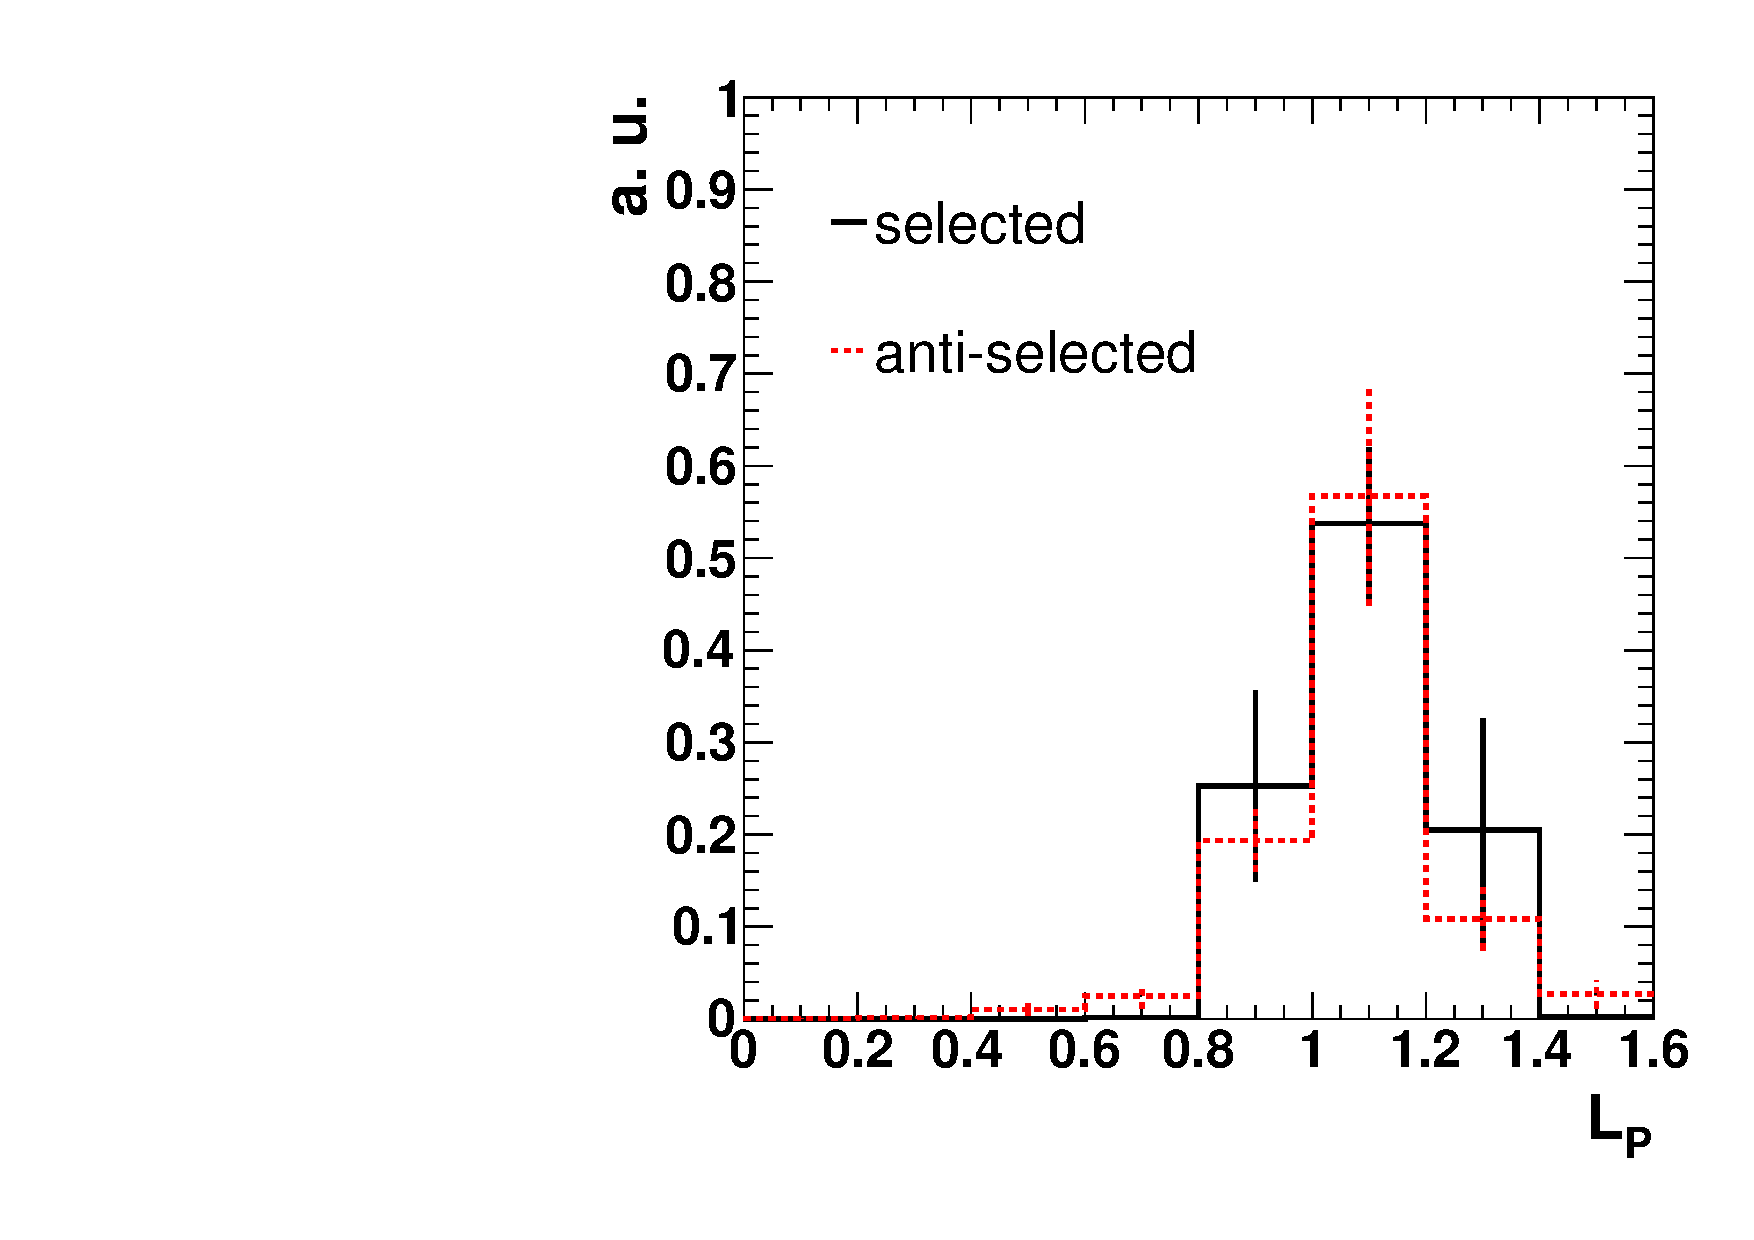
\includegraphics[width=0.5\textwidth]{fig/SelectedVsAntiSelected}}\quad\\
\subfloat[]{\label{fig:susy_elqcd_fitresult150}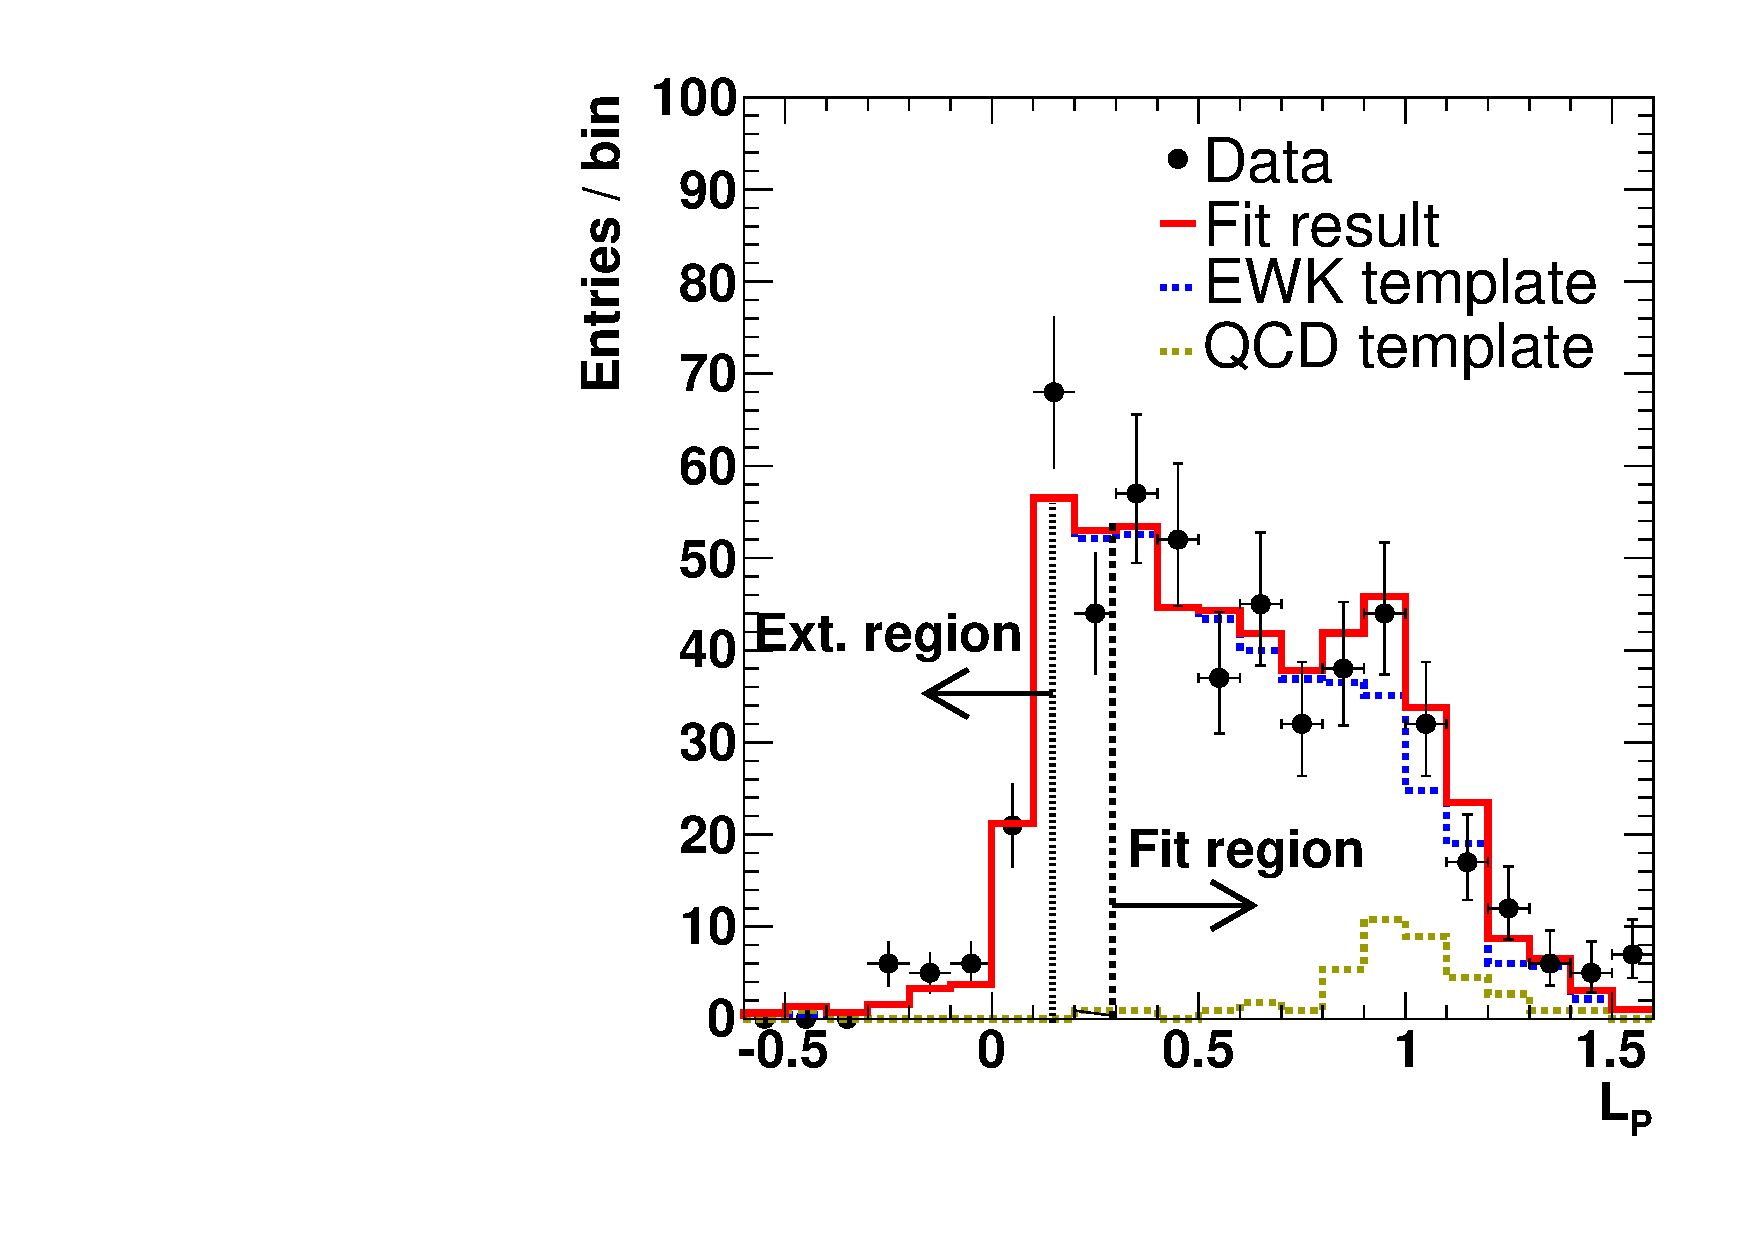
\includegraphics[width=0.4\textwidth]{fig/FitResult_El_150}}\quad
\subfloat[]{\label{fig:susy_elqcd_fitresult250}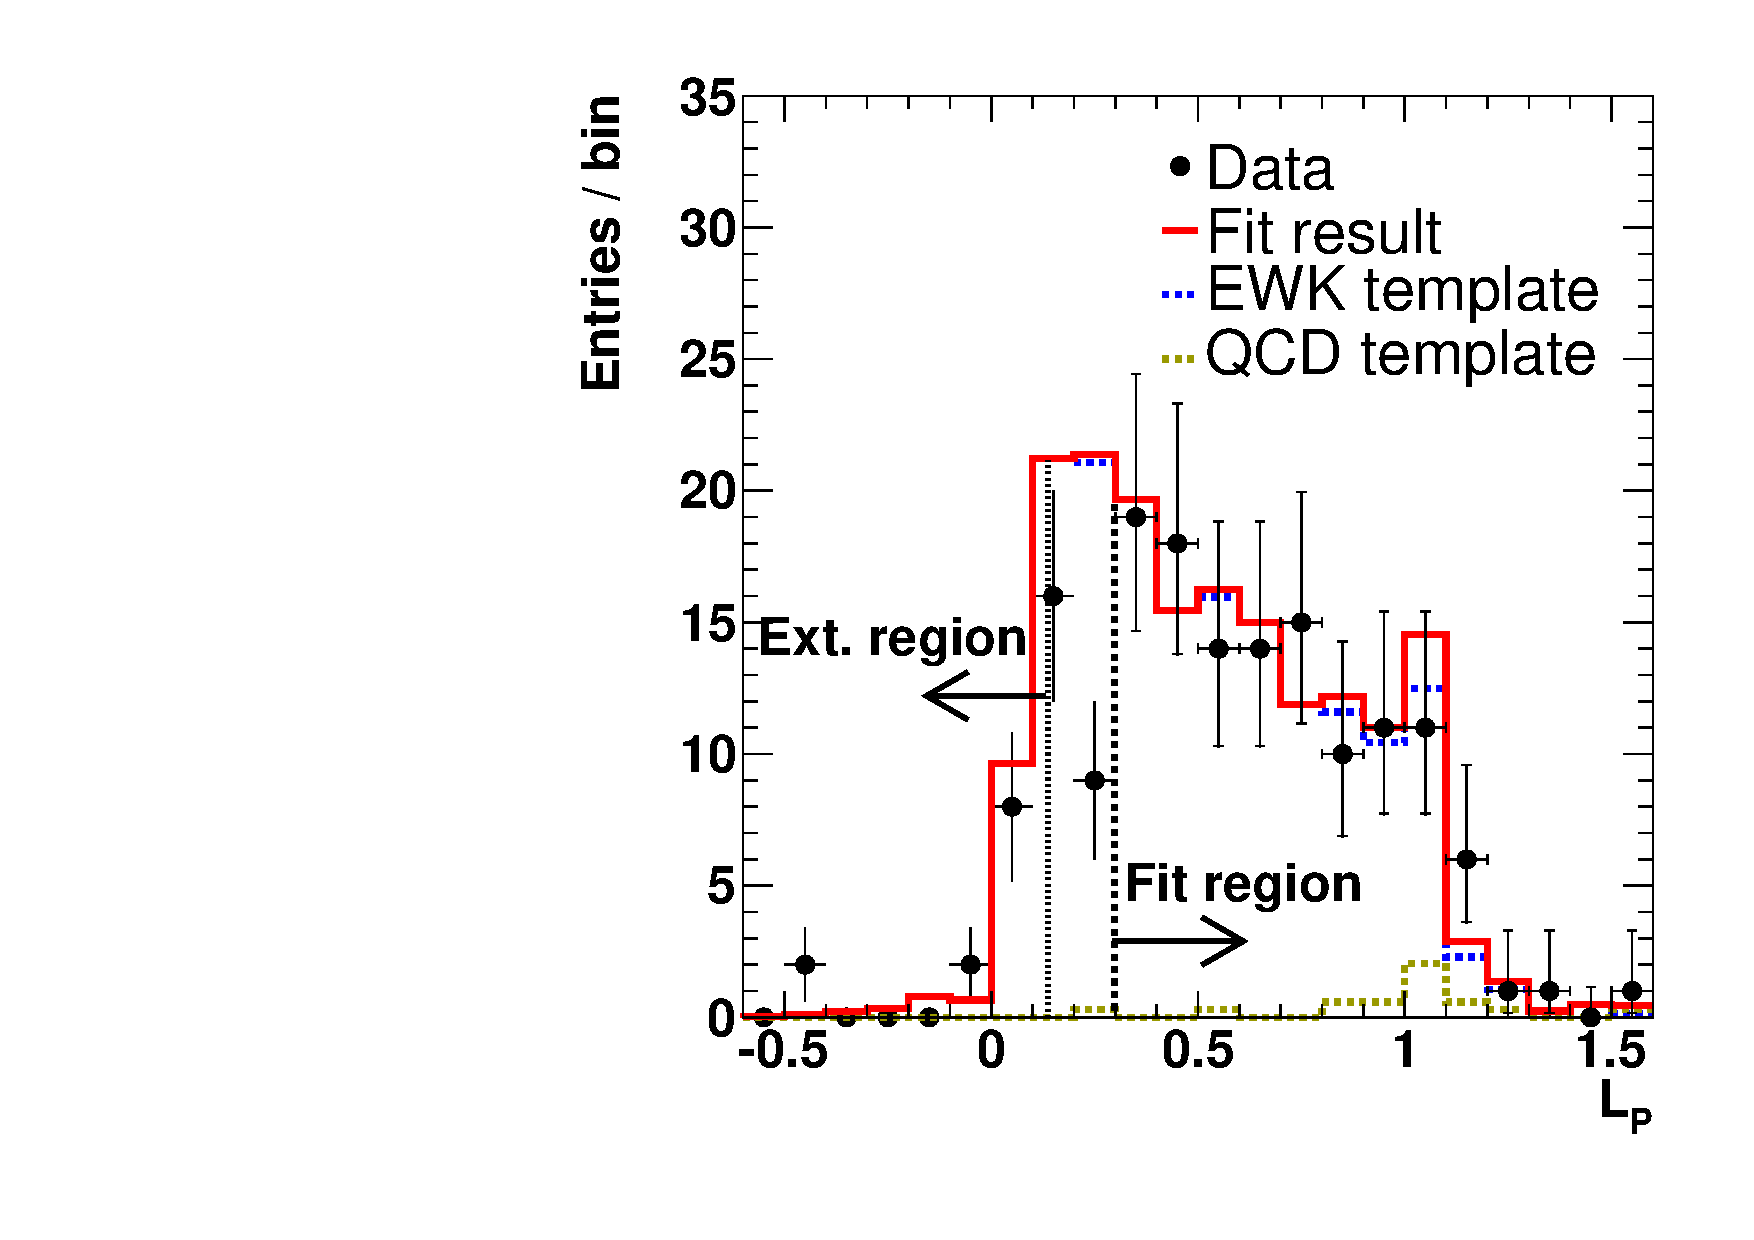
\includegraphics[width=0.4\textwidth]{fig/FitResult_El_250}}
\caption[]{}
\label{fig:susy_elqcd}
\end{figure}

\section{Systematics}
\label{sec:susy_systematics}
For this analysis, as with the \PW polarisation measurement, unavoidable
dependence on simulation requires careful evaluation of associated systematic
uncertainties. It has already been said that the construction of \RCS is
intended to minimise some of these uncertainties by ensuring some degree of
cancellation. Experience from the \PW polarisation measurement showed that the
\LP variable is highly sensitive to certain uncertainties - in particular the
jet energy scale. The size of these uncertainties was thus evaluated early-on in
the development of the analysis and continued throughout. Several of the
systematics procedures were adopted or adapted from those used for the previous
measurement (see Section~\ref{sec:wpol_systematics}).

The background prediction procedure may be written as follows,
\begin{equation}
\NBkgi = \RCSi \times \NControli
\end{equation}
where \NBkgi is the predicted background for \LPsignal in \STlep bin $i$, \RCSi
the corresponding translation factor and \NControli the expected electroweak
yield in the region \LPcontrol (i.e. for the muons, simply the event yield
assuming zero contamination from \ac{QCD} or for electrons, the result of the
fit described in Section~\ref{sec:susy_electron_bgpredict}).

The uncertainty assigned to the background prediction \NBkg must come from two
sources: uncertainty on the translation factor, \RCS and uncertainty on the yield
in the control region, \NControl. These sources of uncertainty will now be
described.

\subsection{Limited Statistics in the Control Region \LPcontrol}
The effect of finite statistics in the control region is naturally more
pronounced in the larger \STlep bins. For the muon channel, this is simply
calculated as the Poisson uncertainty ($\sqrt{N}$) of the number of events in
the control region. For electrons, this uncertainty is taken as the error on the
fitted electroweak component of the background.

\subsection{Limited Monte Carlo Statistics}
\label{sec:susy_syst_mcstats}
The limited statistics of simulated events results in an uncertainty for both
channels in the calculation of \RCS. This is calculated by simple propagation of
errors.

For the electron channel, things are once again complicated by the \ac{QCD}
fitting procedure. The electroweak templates used in the fit also suffer from
limited statistics, thus leading to an additional source of uncertainty on
\NControl. This is accounted for in a similar manner to the statistical
uncertainty of the \ac{QCD} template in the \PW polarisation analysis (see
Section~\ref{sec:wpol_syst_ele_bgest}. The templates are rediced 200 times
according to the statistical error per bin. Each rediced template is then used
to repeat the fit procedure. The variance of this ensemble of fits is then taken
to be the statistical uncertainty. For the systematics quoted in
Table~\ref{tbl:susy_syst_muons}, this is propagated into \RCS. For the limit, as
will be seen, it is taken as an uncertainty on \NControl.

\subsubsection{Jet Energy Scale Uncertainty}
This procedure was changed with respect to the \PW polarisation measurement in
order to harmonise with other analyses. Each jet in the event, as well as the
remaining hadronic recoil are scaled upwards or downwards by 5\%. The larger of
the two shifts on \RCS is then taken as the uncertainty. If the the uncertainty
is found to be smaller than the Monte Carlo statistical error
(Section~\ref{sec:susy_syst_mcstats}), the uncertainty is taken to be the larger
of the two.

\subsubsection{Hadronic Recoil Resolution}
The resolution of the hadronic recoil has previously been measured in
\cite{cms_met_pas}. The resolution measured in data is seen to be 10\% larger
than predicted by simulation. To account for this, the recoil is smeared by an
additional 10\% perpendicular and parallel to its direction. The resulting shift
in \RCS is taken as the uncertainty.

\subsubsection{\Wjets/\ttbar Cross Section}
Te use of \RCS avoids any dependence on the absolute values of theoretical
cross-sections. However, since the \Wjets and \ttbar lead to different \LP
shapes, changes to their relative normalisations will result in changes to
\RCS. To account for this, the \Wjets and \ttbar contributions are each scaled
up and down by 30\% and 50\% respectively. The shift in \RCS with respect to the
unscaled case is then calculated. The shifts are performed simultaneously to
give the most extreme change in \RCS, i.e. one cross-section is shifted up, the
other down. The largest such shift is taken as the uncertainty. As for the jet
energy scale, a shift smaller than the statistical uncertainty of the simulated
sample is taken to be the same as the statistical uncertainty. Additionally, the
uncertainty is calculated simulatenously for both lepton channels in order to
maximise available statistics.

\subsubsection{Muon Momentum Scale}
A bias on the muon momentum is introduced. This is found to be 1\% from studies
of the \PZ mass.

\subsubsection{\PW and \ttbar Polarisation}
The polarisation in \ttbar events is found to be 5\%. Since the effect on \RCS
is less than 5\%, this is assigned as a conservative uncertainty.

For the \PW polarisation, the errors on the previous measurement were taken and
used to assign a 15\% uncertainty to the difference of the left-handed and
right-handed fractions \fLmfR (see Section~\ref{sec:wpol_results}). To account
for this, the simulation was reweighted to reflect and upward and downard shift
of 15\% on \fLmfR with respect to the nominal values. This is done in a manner
similar to that used for the actual measurement (see
Section~\ref{sec:wpol_reweighting}), but using 5 bins in \PtW instead of 3. The
results are shown for the highest \STlep bin in
Figure~\ref{fig:susy_wpol_syst}. The largest of the two shifts is taken to be
the systematic uncertainty.

\begin{figure}
\centering
\subfloat[]{\label{fig:susy_wpol_syst_plus}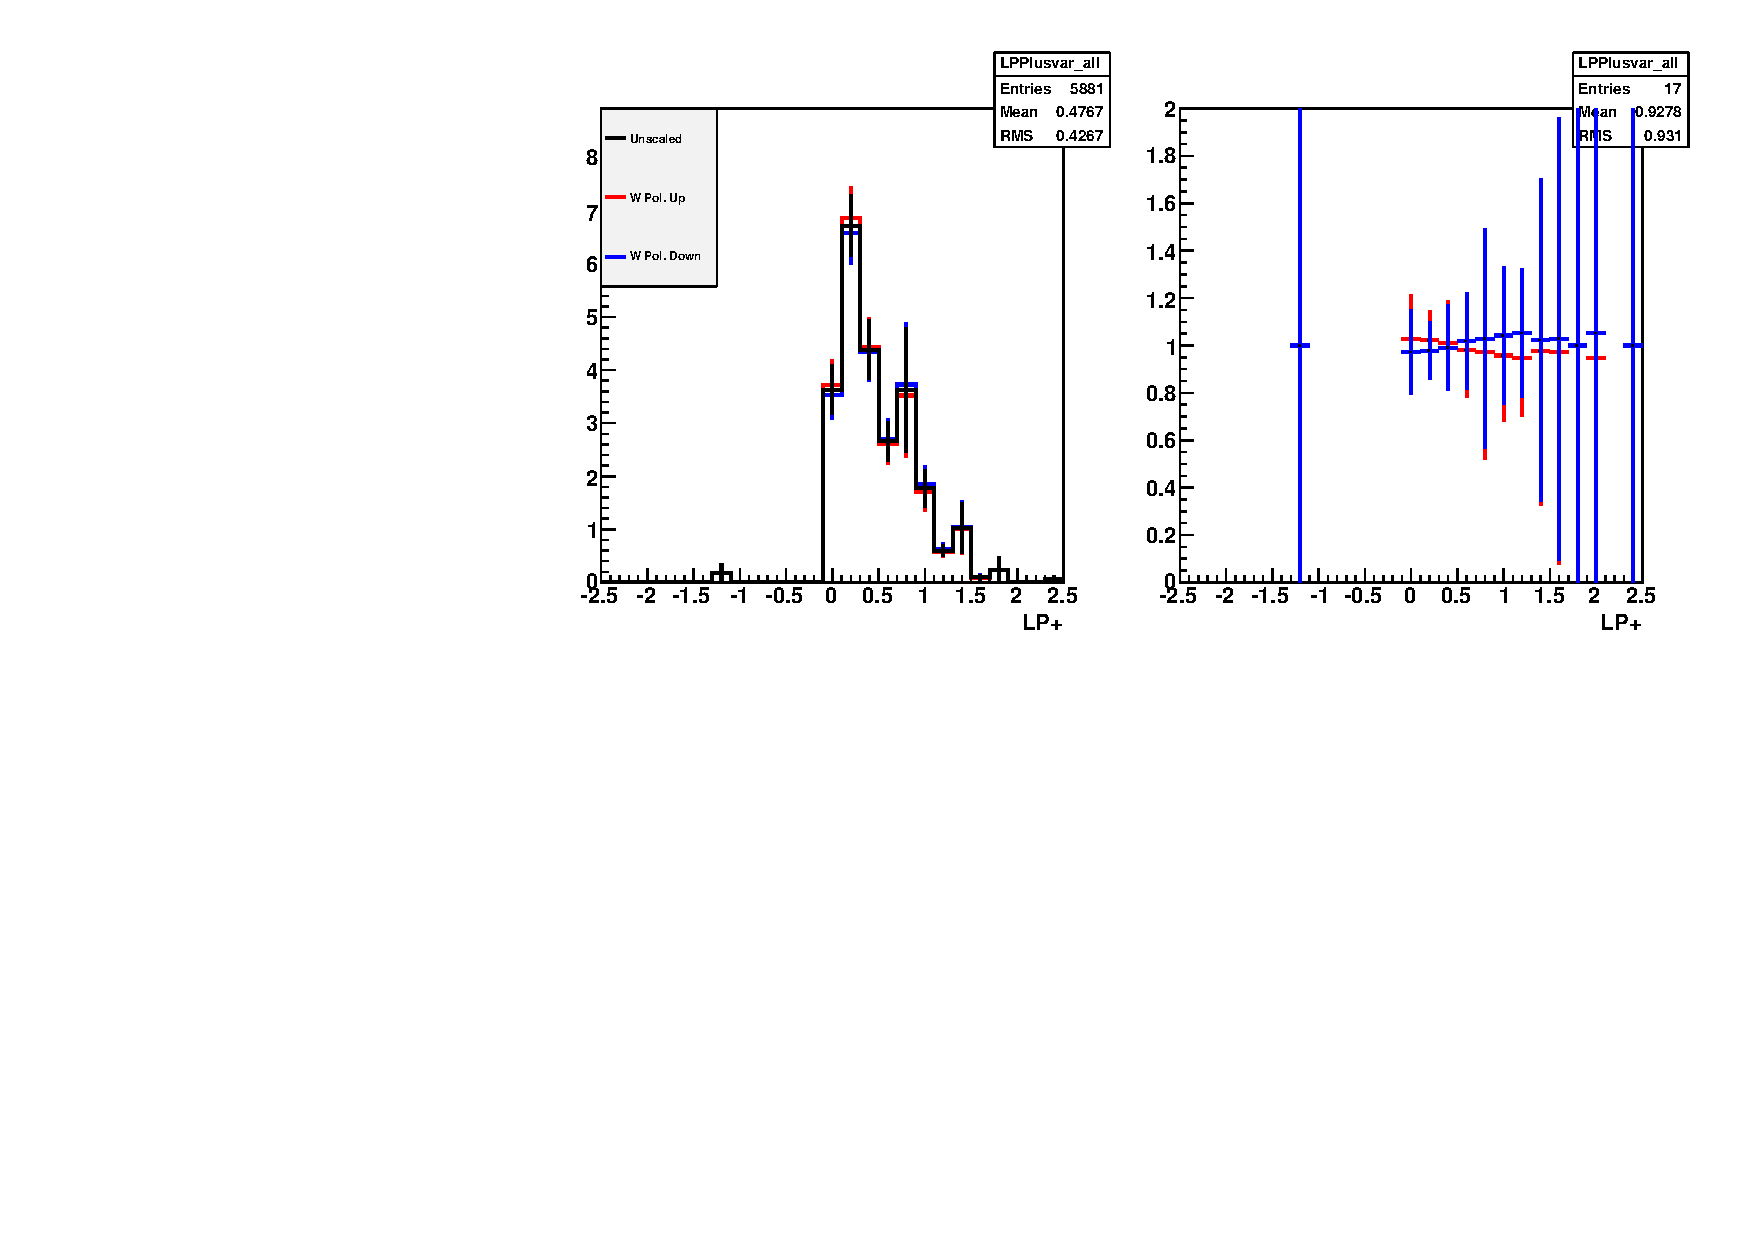
\includegraphics[width=0.9\textwidth]{fig/MuonStandardPlots_450_NOLP_LPPlusvar_all_ratio}}\\
\subfloat[]{\label{fig:susy_wpol_syst_minus}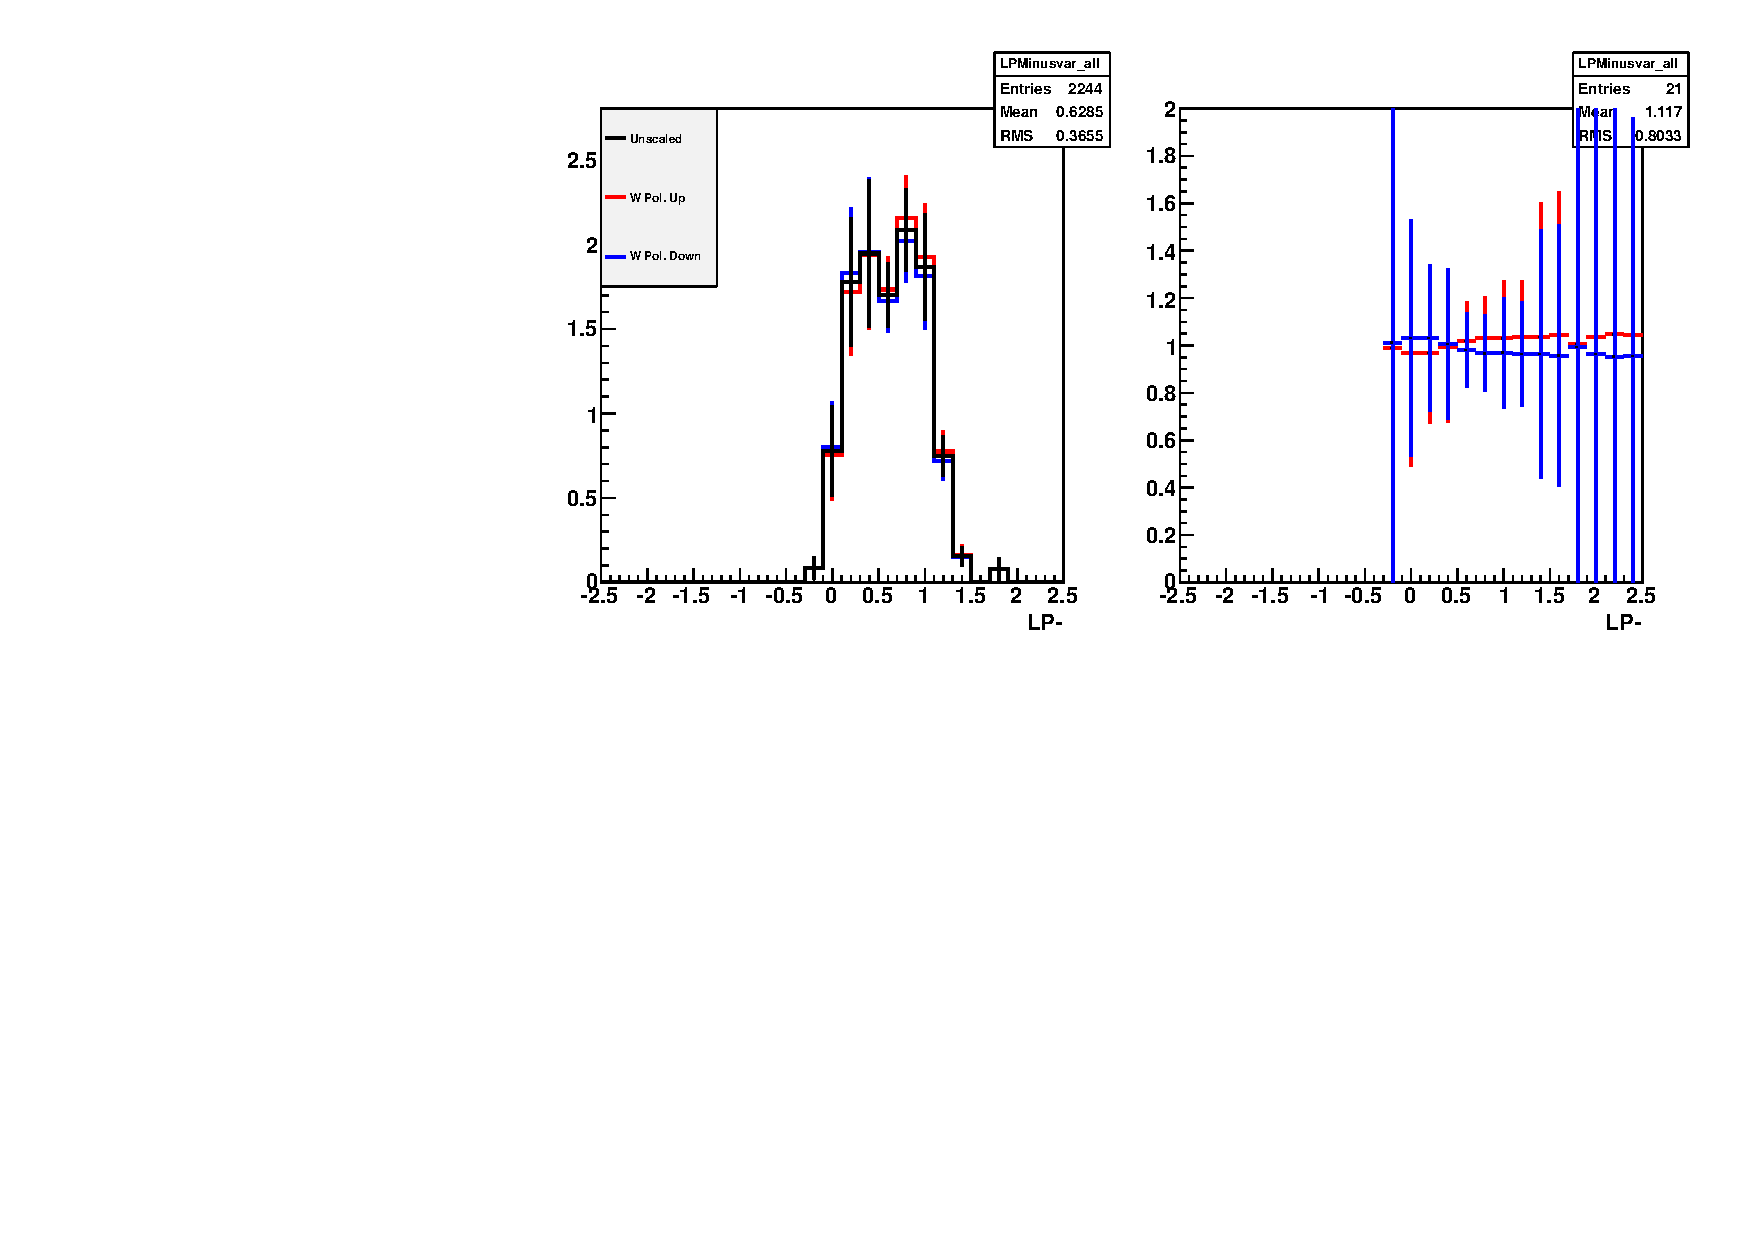
\includegraphics[width=0.9\textwidth]{fig/MuonStandardPlots_450_NOLP_LPMinusvar_all_ratio}}
\caption[]{}
\label{fig:susy_wpol_syst}
\end{figure}

\subsubsection{Fully Leptonic \ttbar}
\subsubsection{\acl{PDF} Uncertainties}
\subsubsection{Trigger Efficiency}
\ctable[
  caption=The relative effects on the values of \f0 and \fLmfR in the muon channel for the uncertainties described. The absolute values are shown in brackets.,
  label=tbl:wpol_mu_syst,
  doinside=\scriptsize
]{ c  p{2.5cm}  p{2.7cm}  p{2.5cm}  p{2.7cm}}{
}{\FL
     Uncertainty                         & $\fLmfR^{-}$                 & $\f0^{-}$                            & $\fLmfR^{+}$                & $\f0^{+}$ \ML
     \ac{JES}                            & $\pm11$\% (0.029)              & $\pm56$\% (0.123)       & $\pm3$\% (0.011)   & $\pm42$\% (0.092) \NN
     \MET Resolution                     & $\pm4$\% (0.012)               & $\pm3$\% (0.006)        & $\pm4$\% (0.012)   & $\pm2$\% (0.004)                        \NN
     $P_T(\mu)$ bias: $\pm$1\%/100 GeV   & $\mp$0.8\% (0.002)             & $\mp$ 11\% (0.004)      & $\pm1.2$\% (0.004) & $\mp$16.0\% (0.036)                   \ML
     Quadratic sum                       & $\pm12$\% (0.031)              & $\pm56$\% (0.123)       & $\pm5$\% (0.017)   & $\pm45$\% (0.099) \LL
}
\ctable[
cap=Systematic uncertainties in the electron channel,
caption={Sources of systematic uncertainty and their effect on the translation
factor, $R_{CS}$, in the electron channel. The relative uncertainty on the estimated number of events in the
signal region, stemming from the limited yield in the control
region, is also listed.},
pos=ht,
label=tbl:susy_syst_electrons
]{lcccc}{
}{\FL
                                   & \multicolumn{4}{c}{  \STlep Range (GeV) }\ML
                                   & [150-250] & [250-350] & [350-450] & $>$ 450\ML
$R_{CS}$                           & 0.16      & 0.18      & 0.19      & 0.23\ML
%$\Delta N/N$ at 1.1~fb$^{-1}$ (\%) & 12        & 22        & 38        & 58\ML
Systematic Uncertainty (\%)        & 14        & 20        & 24        & 34 \ML
Control Region Stat.      (\%)     & 5         & 9         & 17        & 24\NN
MC Stat.       (\%)                & 1         & 10        & 7         & 8 \NN
\ac{JES} (Flat 5\%)(\%)            & 9         & 10        & 10        & 19 \NN
\MET Resolution (10\%) (\%)         & 2         & 2         & 5         & 7 \NN
W/\ttbar Ratio (\%)                & 6         & 7         & 6         & 10 \NN
\ttbar($\ell\ell$) (\%)            & 6         & 7         & 6         & 2\NN
W Polarization (\%)                & 1         & 1         & 2         & 3\NN
\ttbar Polarization (\%)           & 5         & 5         & 5         & 5 \LL
}

\section{Results}
\begin{figure}
\centering
\subfloat[]{\label{fig:susy_mu_lp250}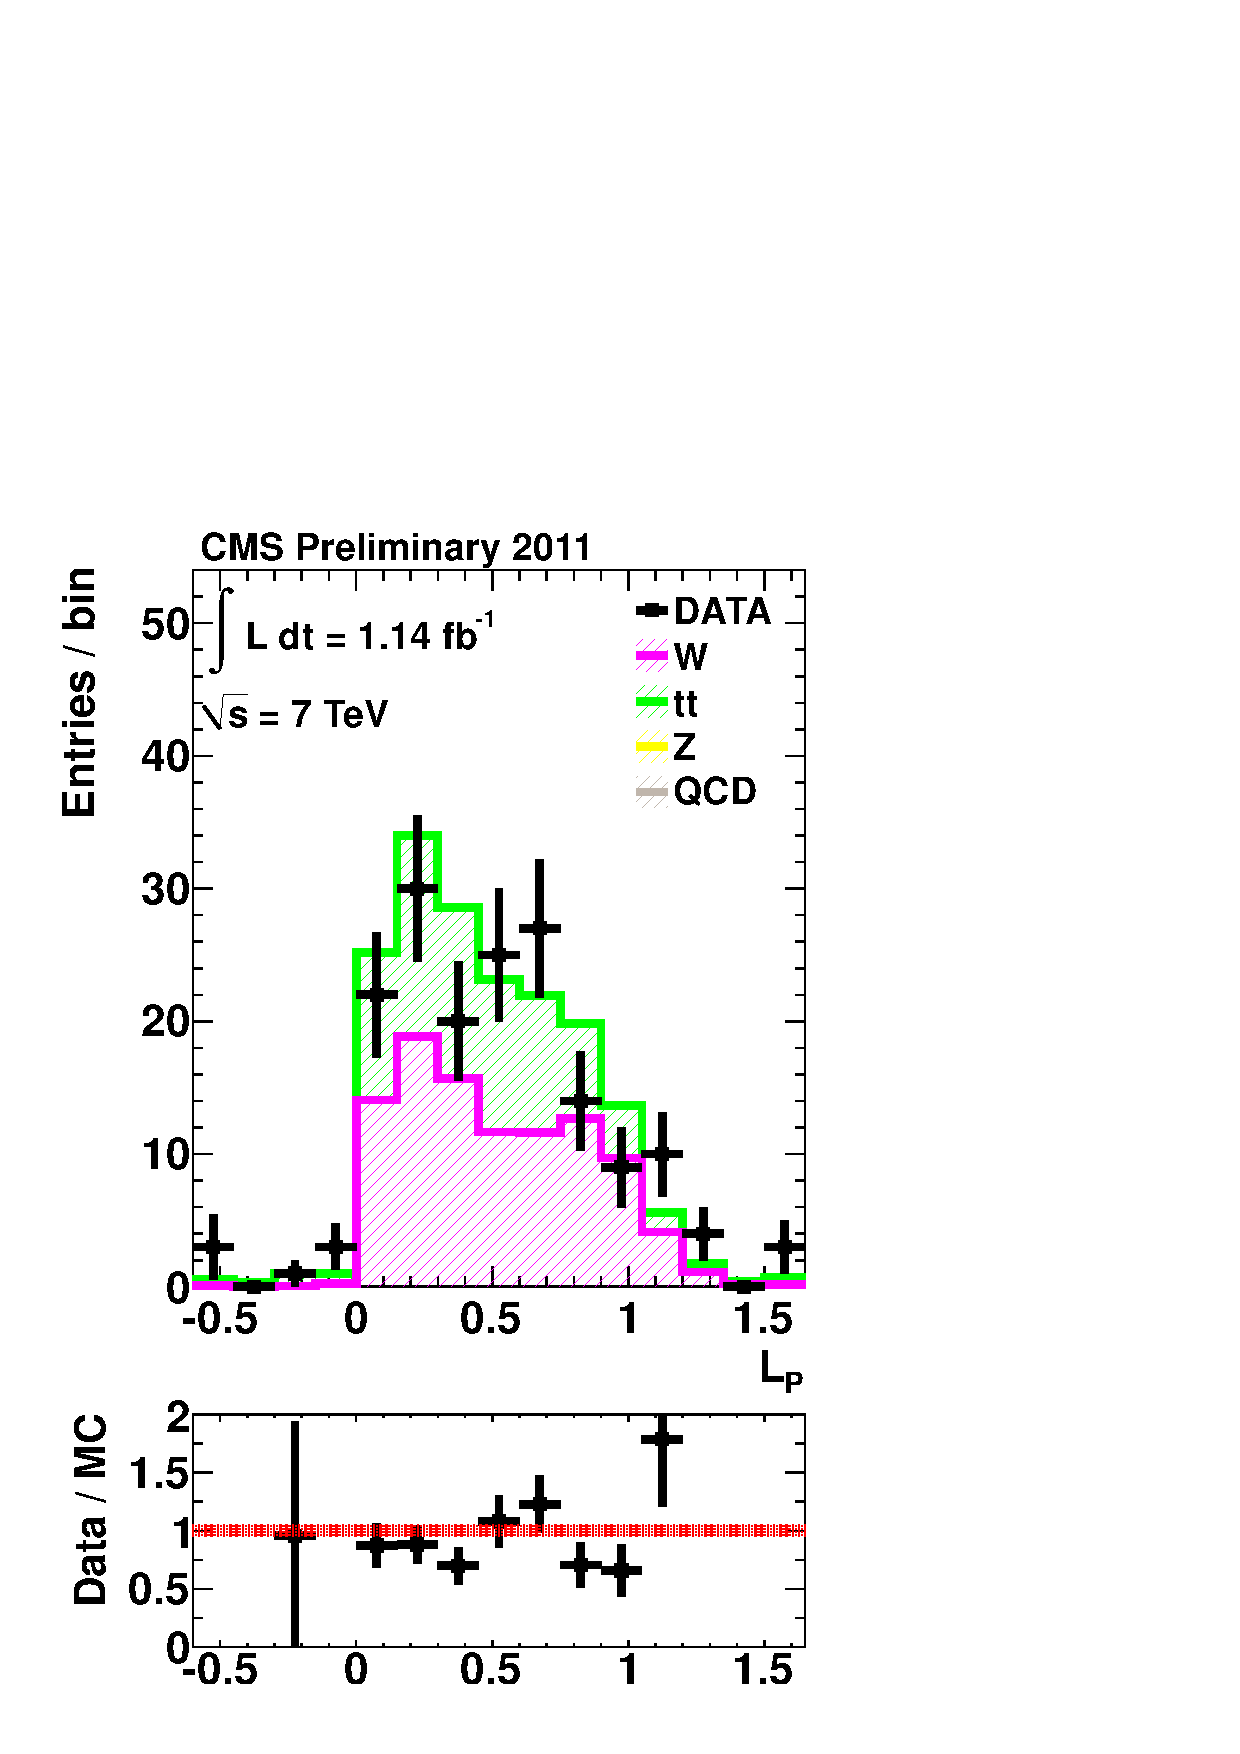
\includegraphics[width=0.3\textwidth]{fig/MuHad_LP250}}\quad
\subfloat[]{\label{fig:susy_mu_lp350}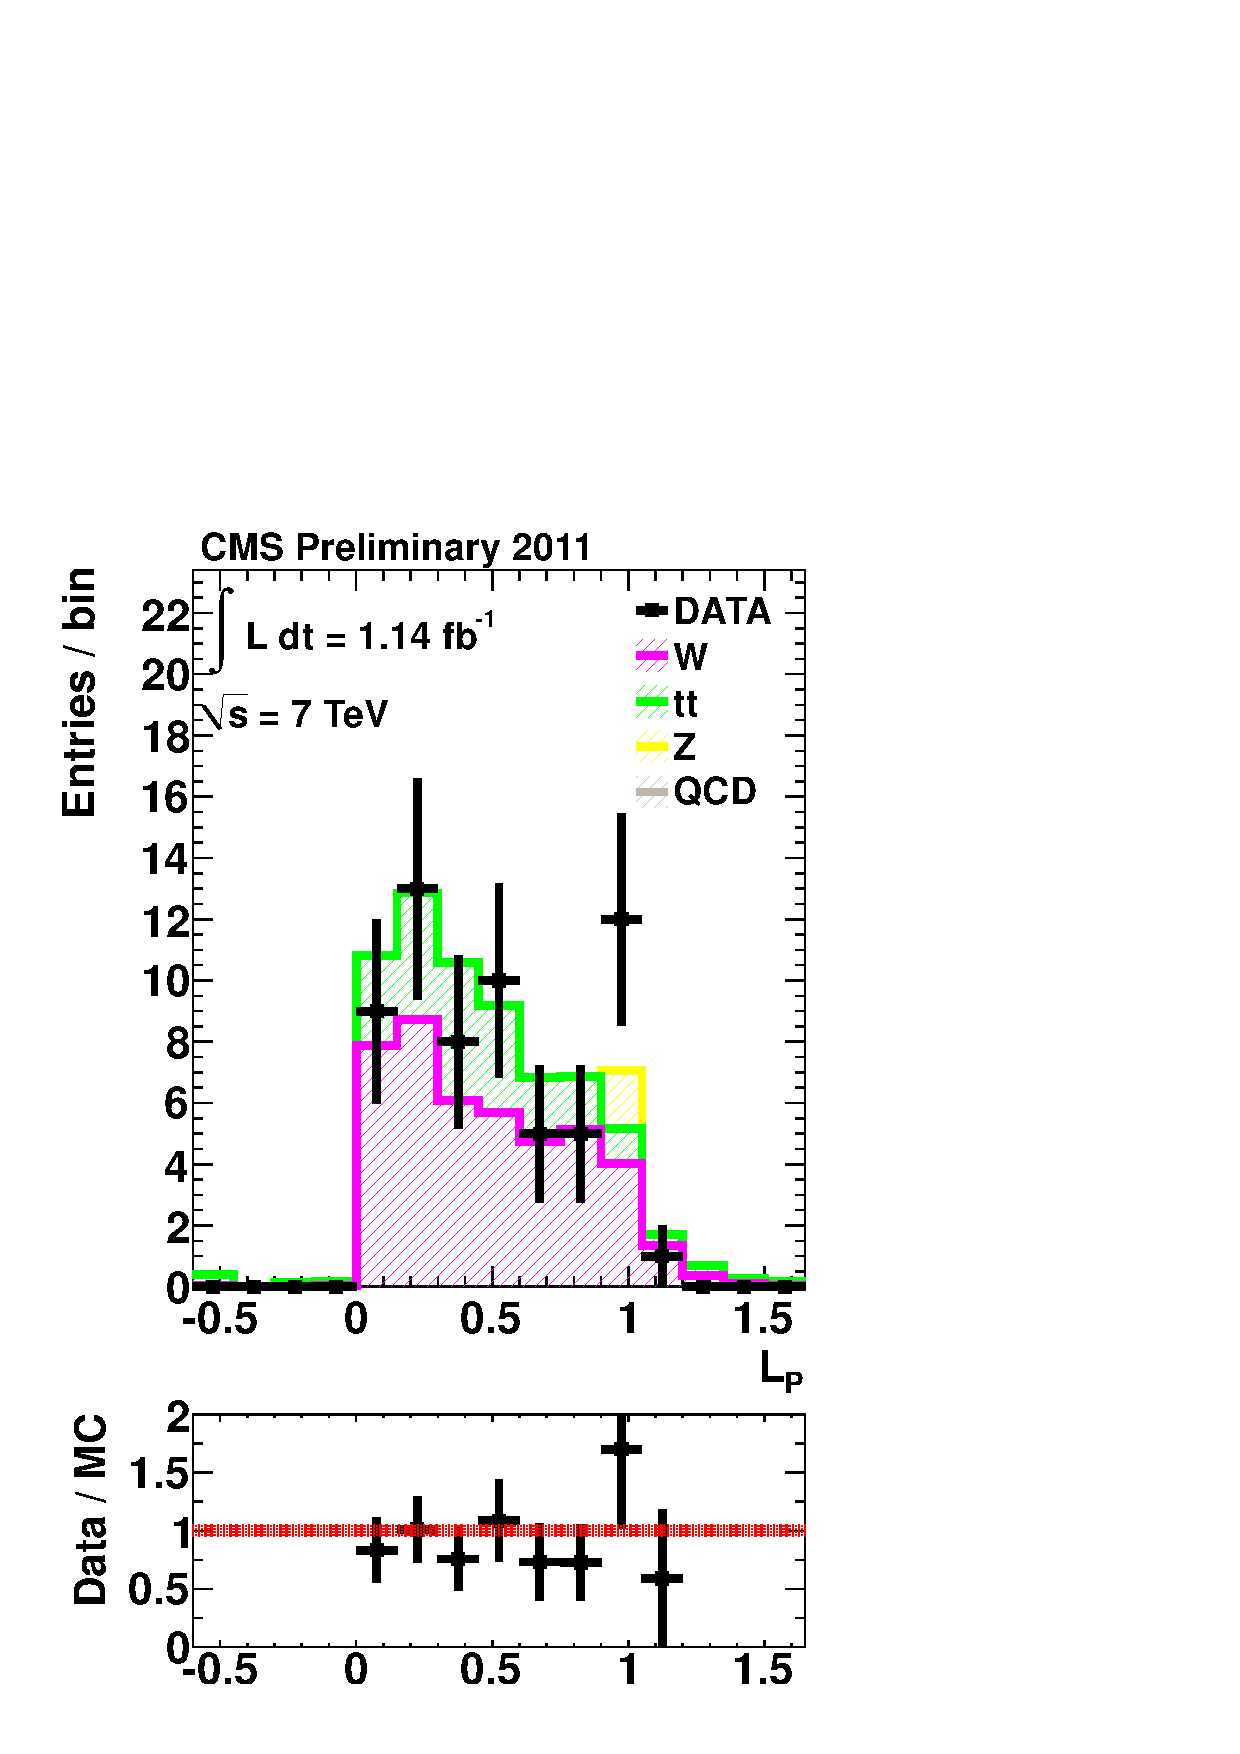
\includegraphics[width=0.3\textwidth]{fig/MuHad_LP350}}\quad
\subfloat[]{\label{fig:susy_mu_lp450}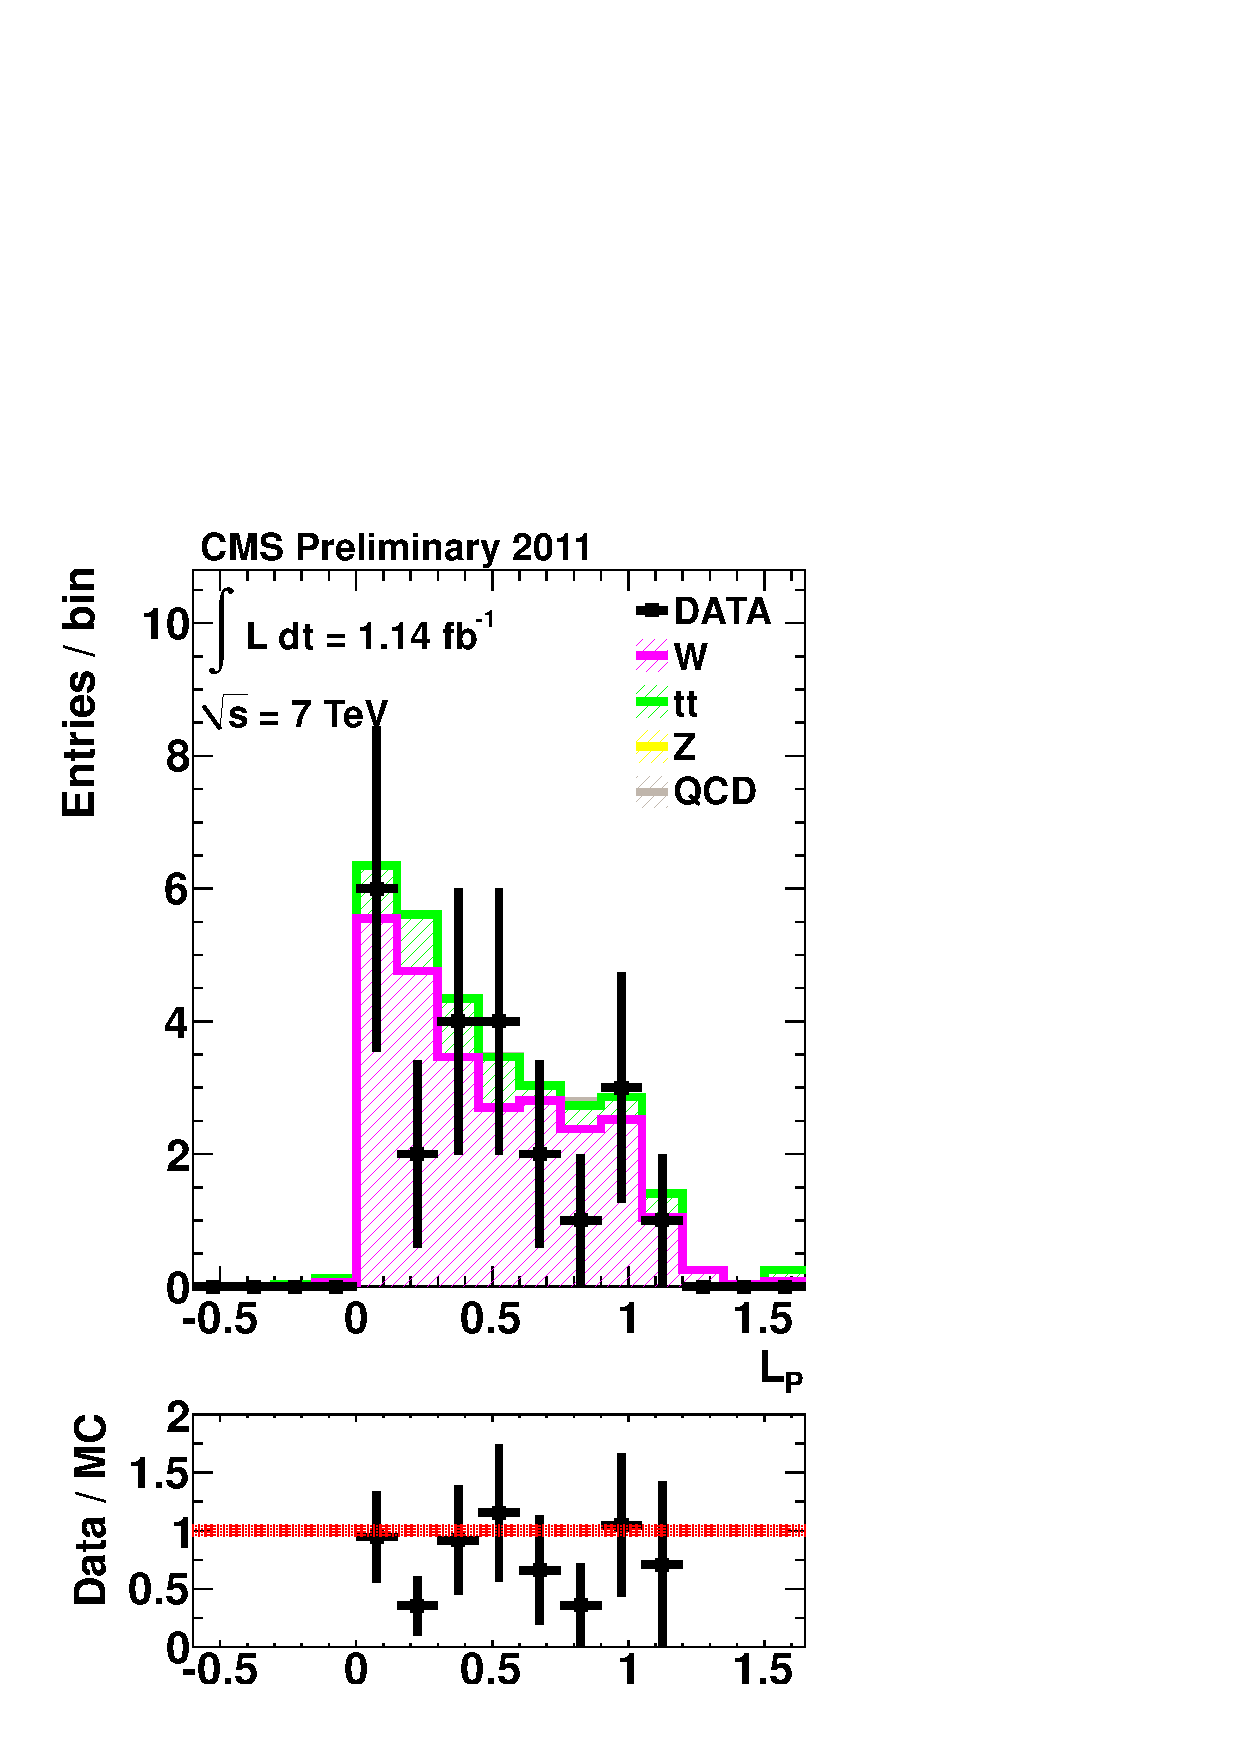
\includegraphics[width=0.3\textwidth]{fig/MuHad_LP450}}\\
\subfloat[]{\label{fig:susy_el_lp250}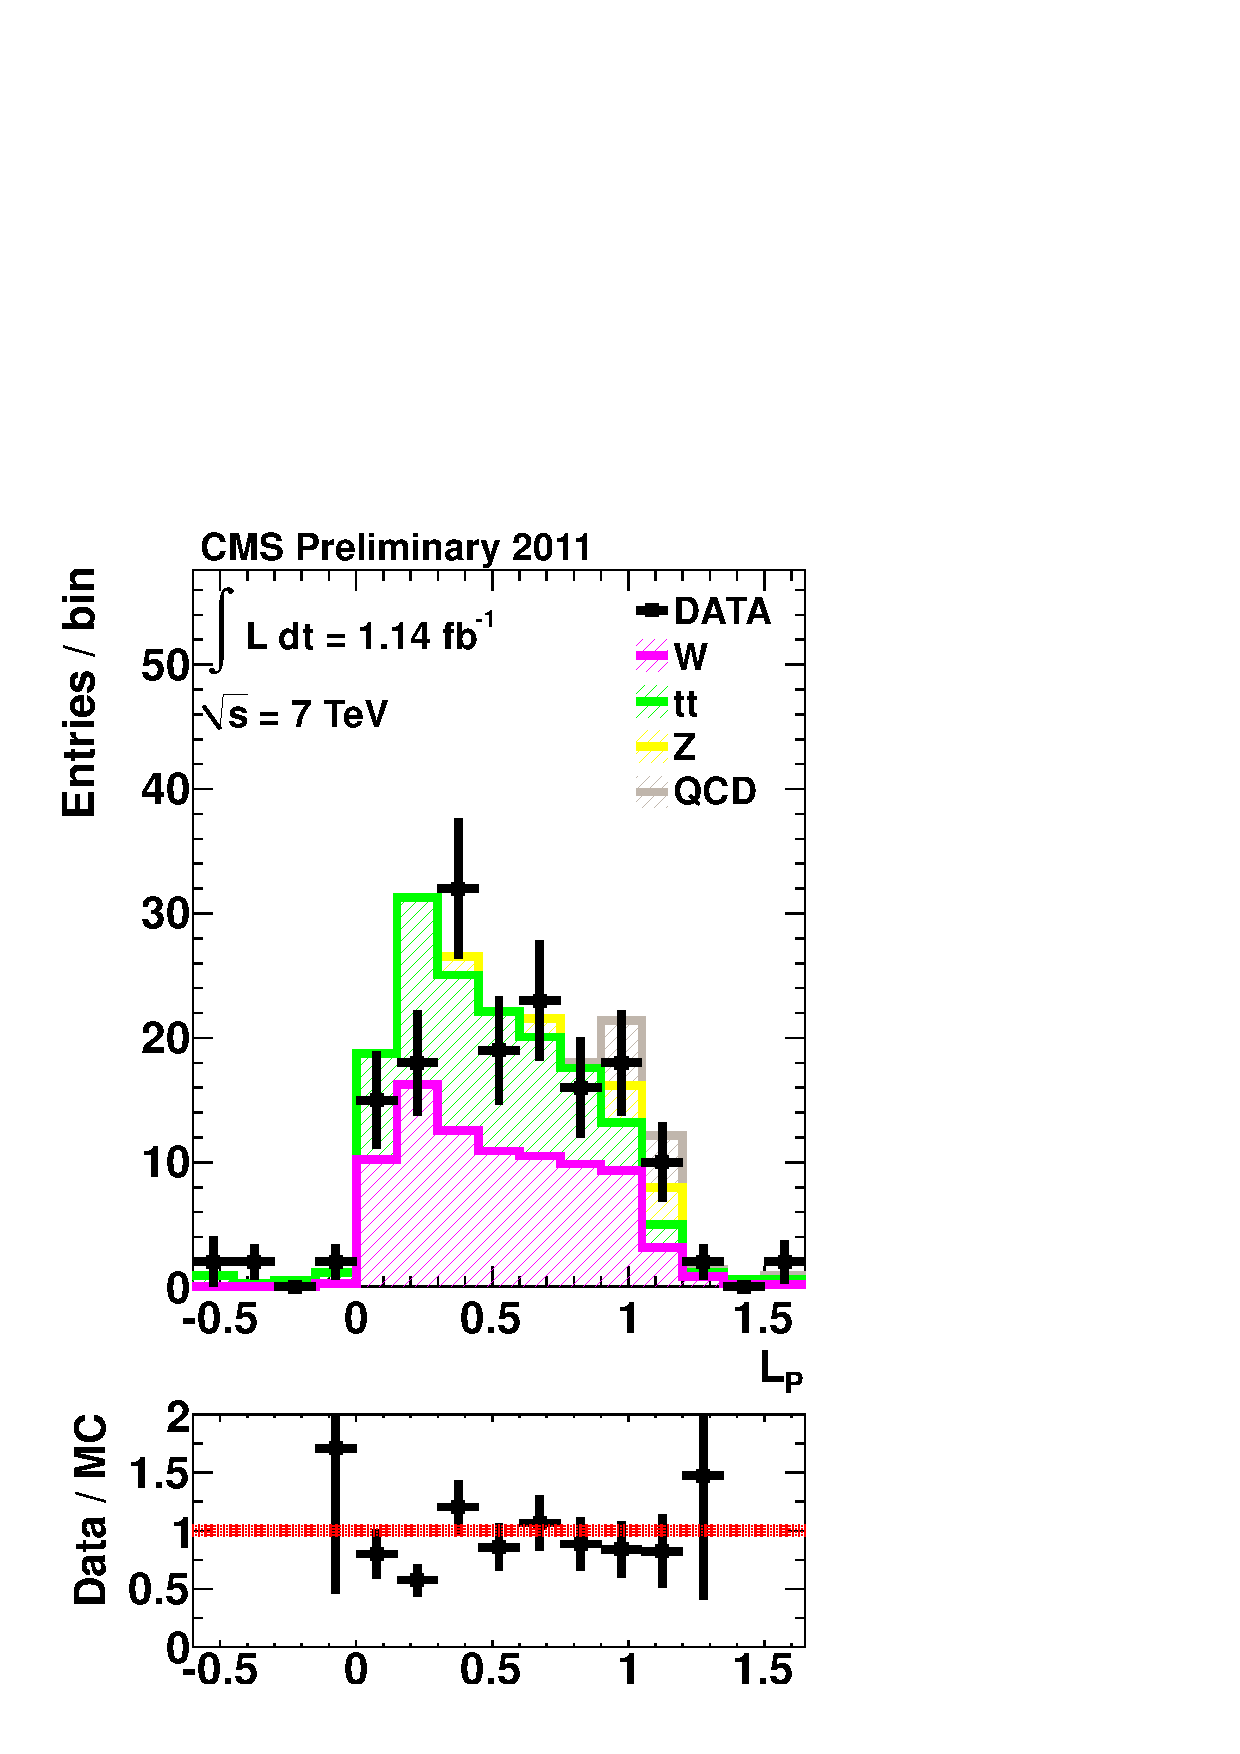
\includegraphics[width=0.3\textwidth]{fig/ElHad_LP250}}\quad
\subfloat[]{\label{fig:susy_el_lp350}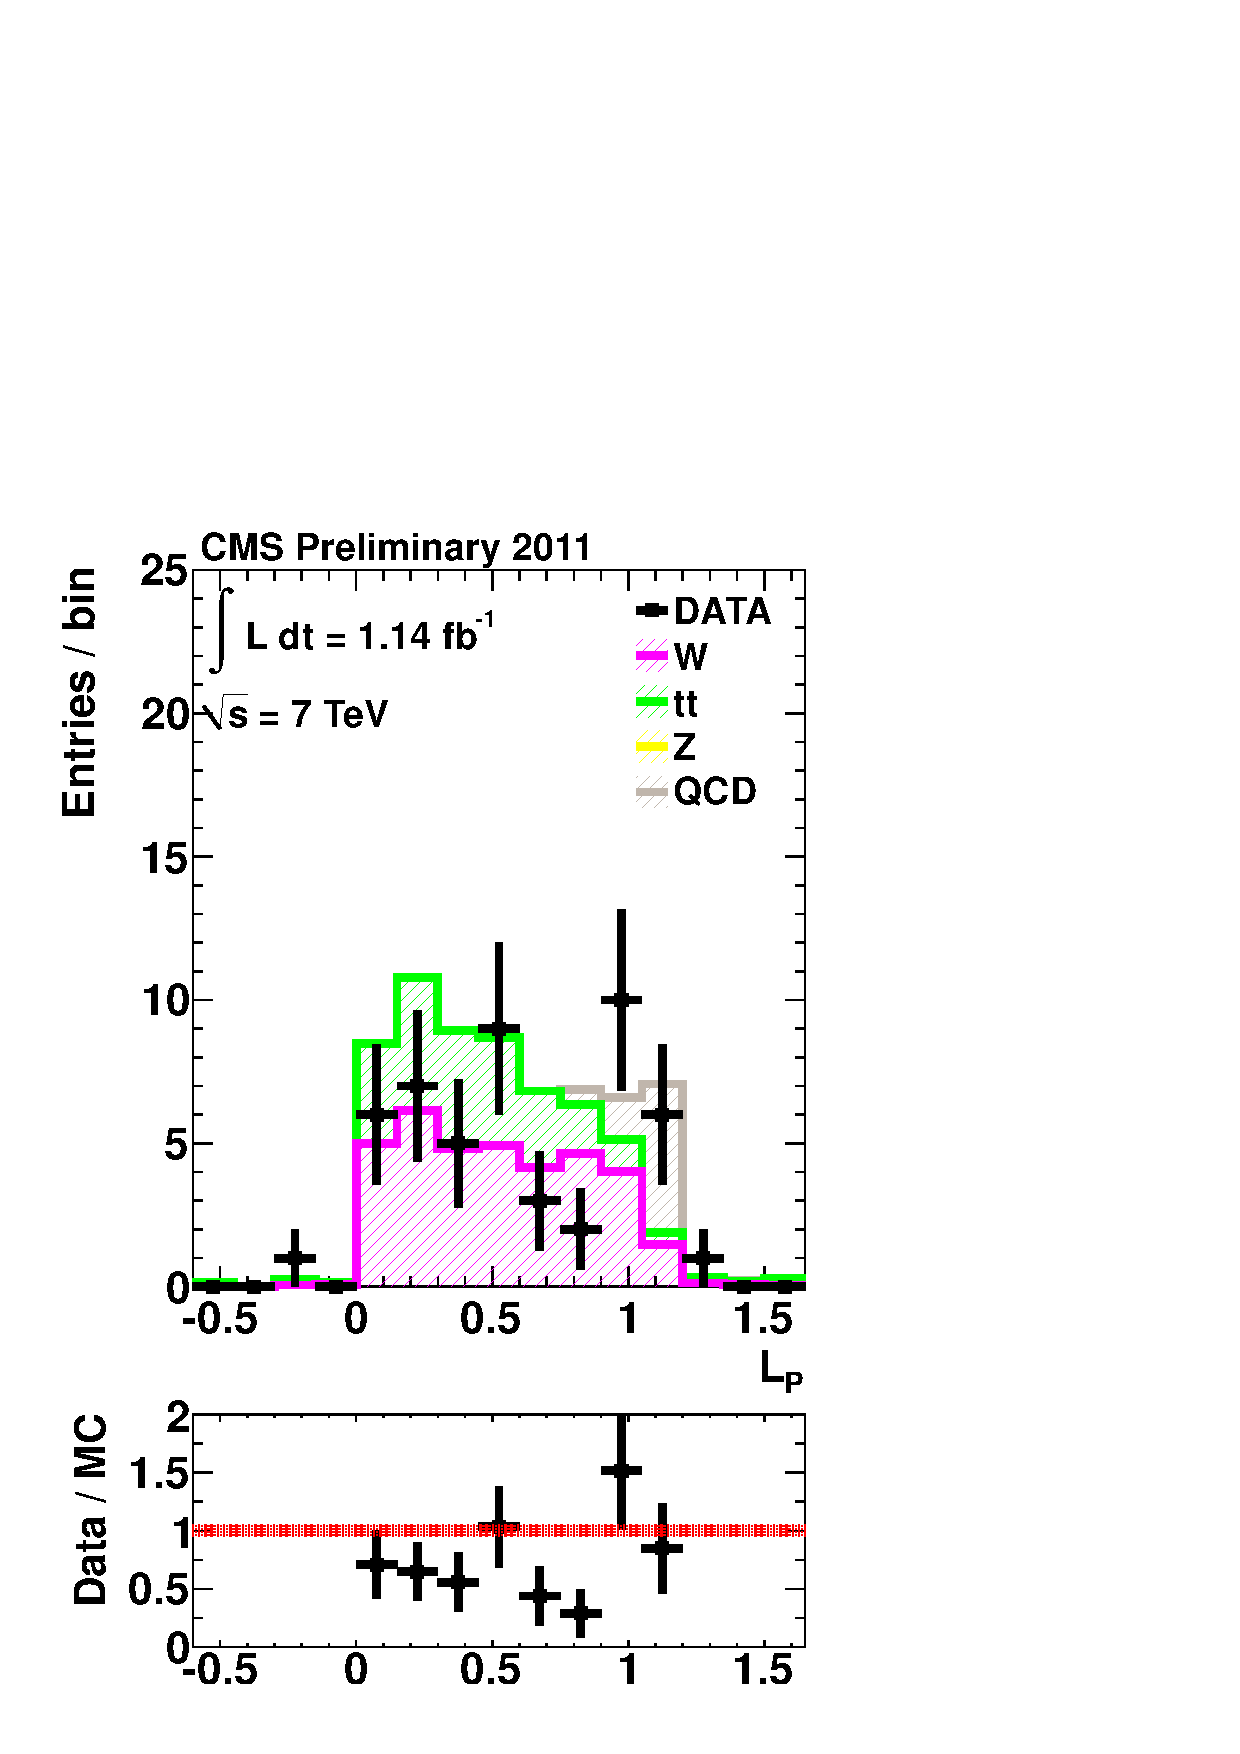
\includegraphics[width=0.3\textwidth]{fig/ElHad_LP350}}\quad
\subfloat[]{\label{fig:susy_el_lp450}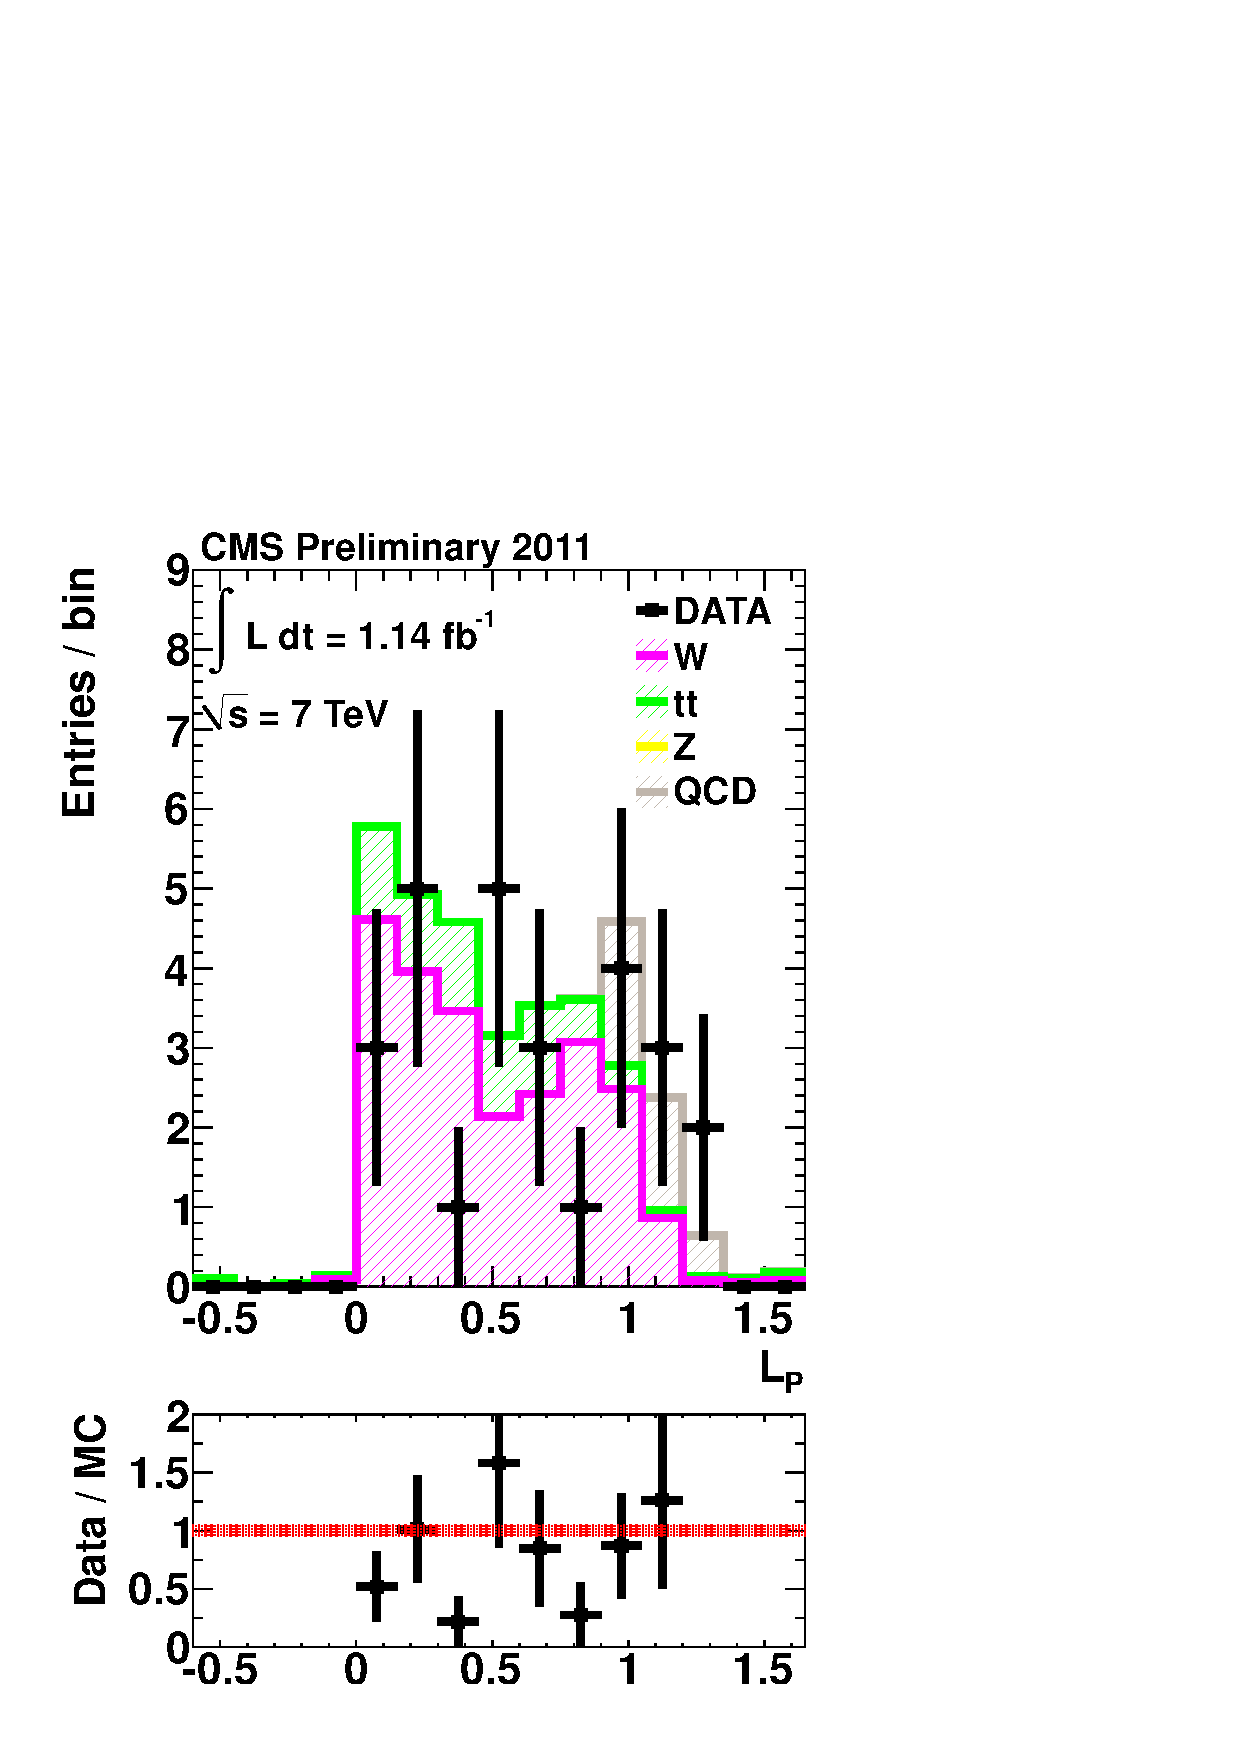
\includegraphics[width=0.3\textwidth]{fig/ElHad_LP450}}
\caption[]{}
\label{fig:susy_datamc}
\end{figure}

\begin{figure}[htb]
\centering
\subfloat[]{\label{fig:susy_pred_mu}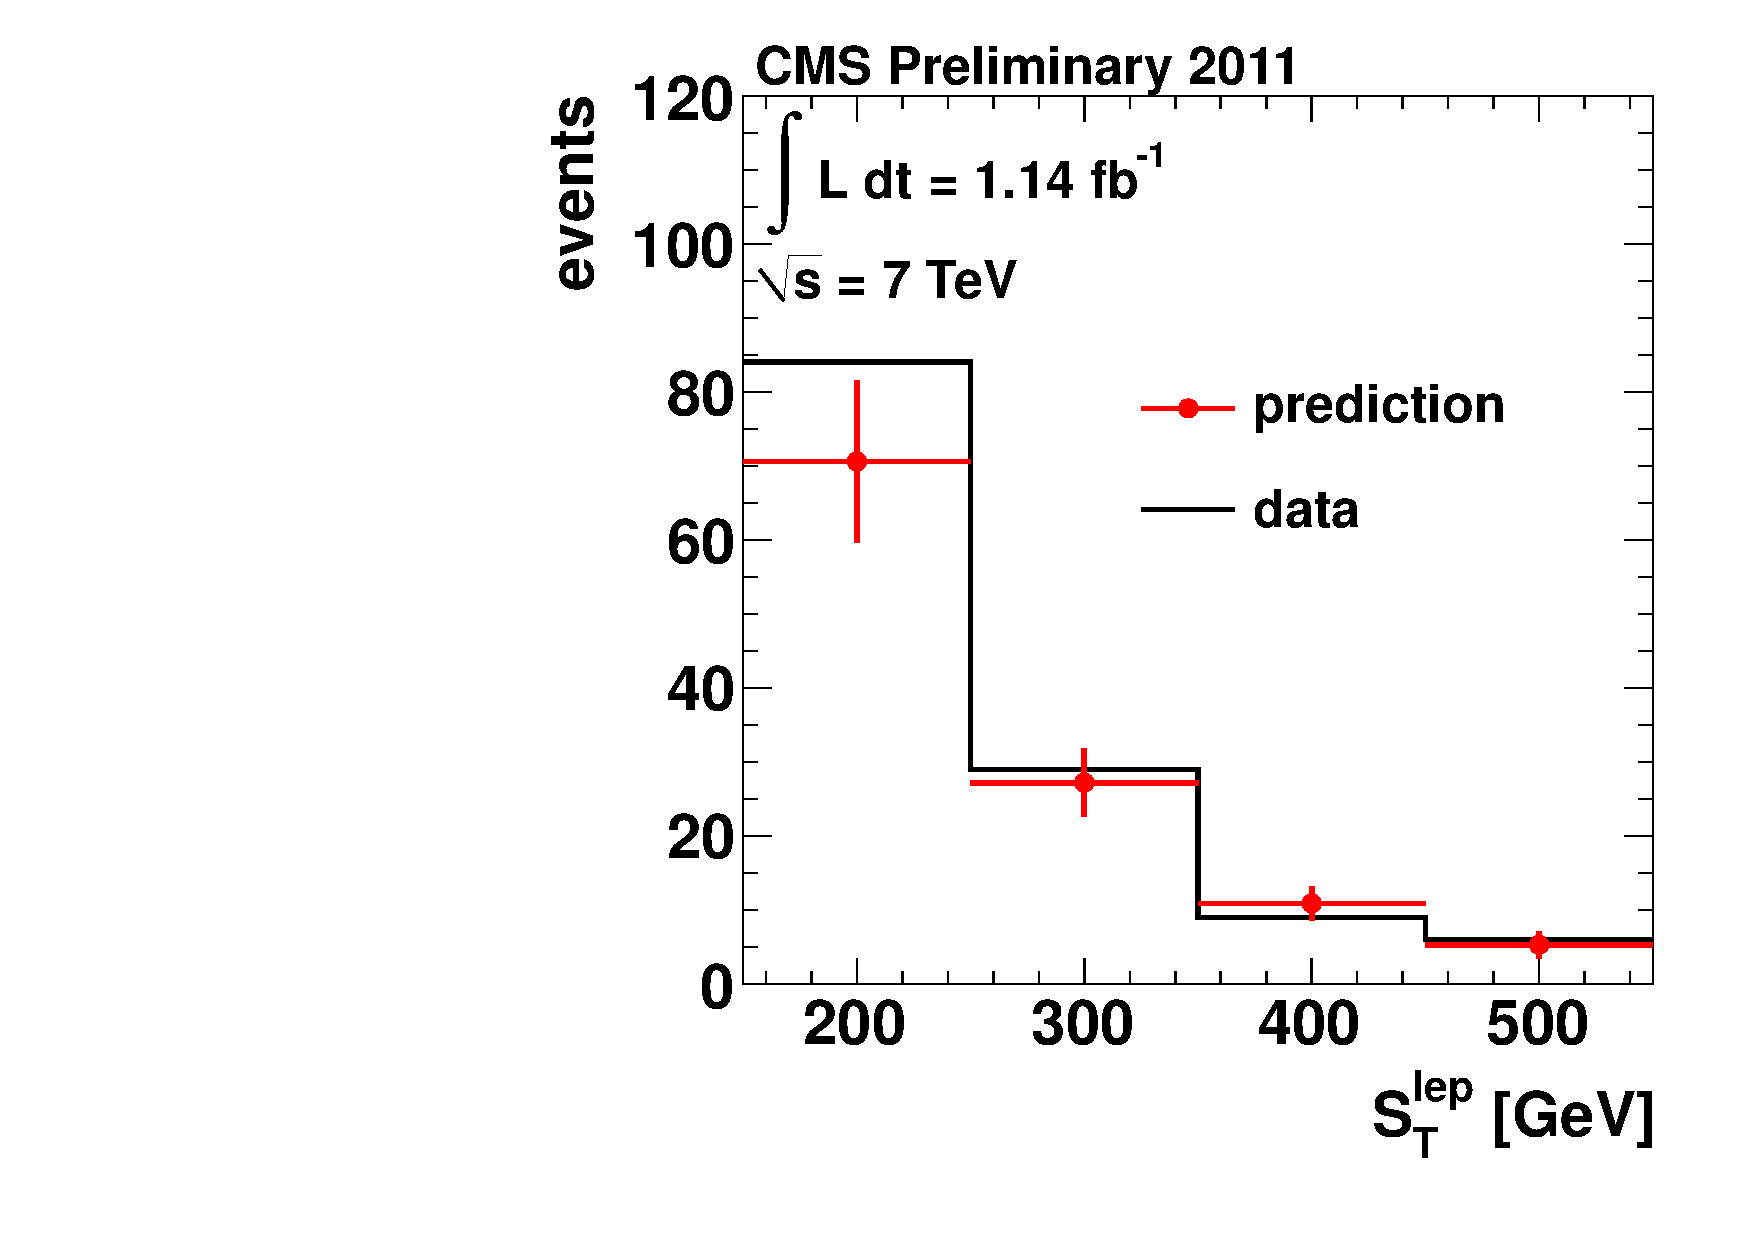
\includegraphics[width=0.4\textwidth]{fig/prediction_mu}}\quad
\subfloat[]{\label{fig:susy_pred_el}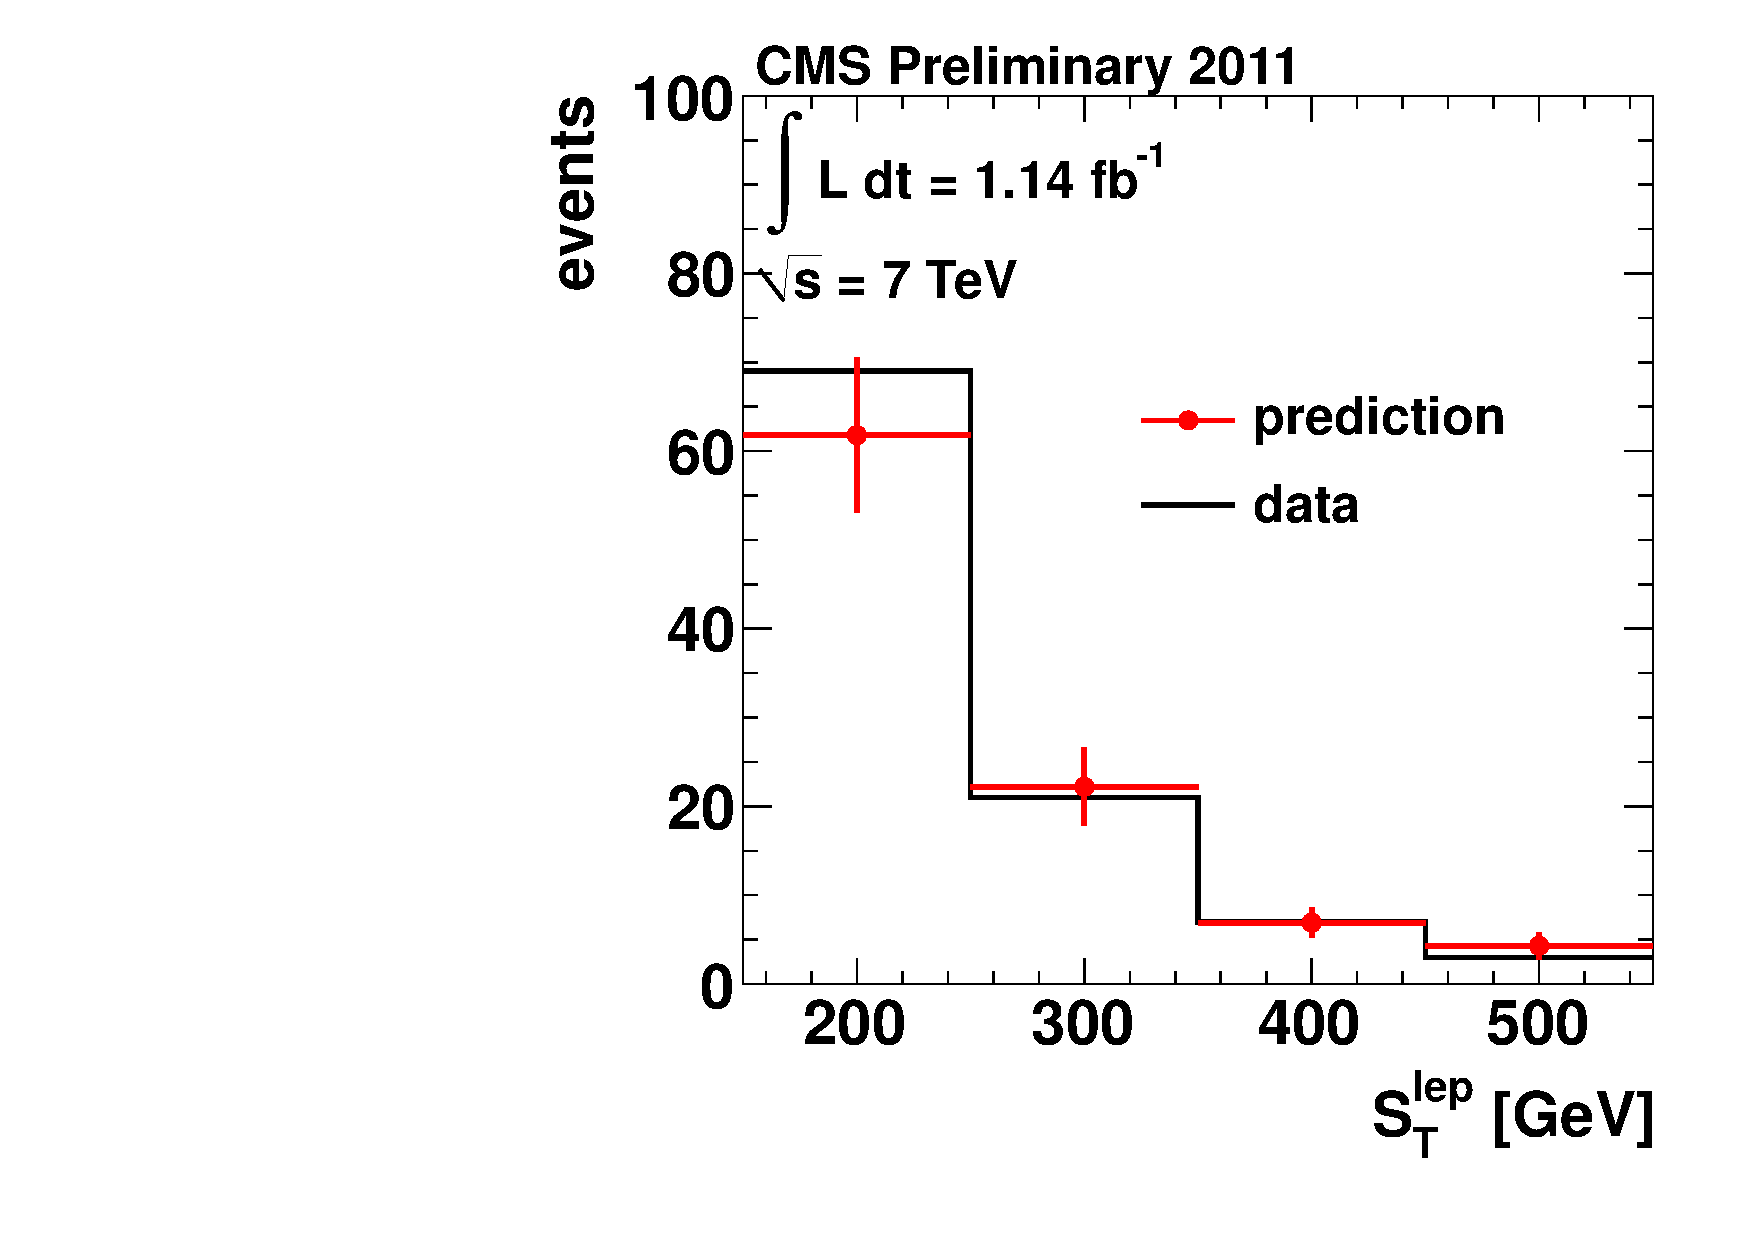
\includegraphics[width=0.4\textwidth]{fig/prediction_el}}\quad
\caption[]{Comparison of the number of events observed in the data and the
  expectations from the background estimation methods presented above, in the
  different \STlep bins.\subref{fig:susy_pred_mu} muon channel;
  \subref{fig:susy_pred_el} Electron channel.  The red error-bars indicate the
  statistical uncertainty of the data only.}
\label{fig:susy_pred}
\end{figure}
  \chapter{Interpretation of Search Results Within Theoretical Models}
\label{sec:interpretation}
\section{Introduction}
It is very often the case that a search for \ac{NP} will yield results
consistent with the currently accepted theory (which, in most particle physics
contexts would be the \ac{SM}). In the absence of a discovery\footnote{Certain
  models may also have a role to play in the characterisation of a discovery.},
it is often desirable to provide additional information in the form of a
statistical interpretation of the results. Such an interpretation typically
serves the following goals:
\begin{itemize}
\item Indicate the strength of the analysis in searching for the proposed model
  or set of models. This can then be used as an objective measure by which to
  rank different analyses or to benchmark the progress of a single analysis as
  data is collected.
\item Falsify, to some confidence level, a particular theory or some region of
  parameter space within that theory. In the case of a reasonably generic model,
  parameterised in such a way that it may represent other theories (or
  approximate their experimental signature), theorists may be able to
  test the predictions of a variety of models directly against the results of
  the interpretation. This will be discussed further in Section~\ref{sec:sms}.
\item Guide the optimisation of analysis cuts and object selection.
\end{itemize}

Providing an interpretation invariably necessitates some choice of theory or
phenomenological model against which to test the results. The range of theories
will of course depend strongly on the inclusiveness of the experiment. Indeed,
in many cases a single theory will have motivated the analysis in the first
place and the choice of model will be clear. In other cases, the analysis have
been designed to be as inclusive as possible and therefore sensitive to an array
of theories. Typically this is achieved by focussing on a particular detector
signature (for instance missing transverse energy), where a deviation from the
\ac{SM} is a common feature of many \ac{NP} scenarios. Another similar issue
arises when the model being tested is not well defined with a large number of
free parameters which affect the experimental expectations.

\ac{SUSY} searches in particular are subject to these
considerationss. Firstly, as discussed in Section~\ref{sec:susy}, the theory
has a large number of free parameters which may drastically change the
experimental signature. Secondly, whilst a \ac{SUSY} specific interpretation is
possible in principal, it is in some sense not the best use of the experimental
data. The large, multi-dimensional \ac{SUSY} parameter space and corresponding
variation in the physics signatures necessitates an inclusive analysis
strategy - typically looking for high jet multiplicities in association with
large missing transverse energy. Such signatures may occur in a variety of
potential \ac{NP} theories. With an appropriate interpretation, the results of
an inclusive \ac{SUSY} search can be used to draw conclusions about these
theories, restricting their parameter space or ruling them out altogether.

\ac{SUSY} searches at the \ac{LHC} have typically provided two
interpretations. The first, within a very restricted class of \ac{SUSY} theories
known as the \ac{CMSSM}. The second, within one or more so-called ``Simplified
Models'', chosen by theorists to represent a wide range of possible \ac{NP}
theories, categorised according to their phenomenological properties.

\section{Models}
\subsection{\acl{CMSSM}}

\subsection{Simplified Models}
\label{sec:sms}
It is often the case that theorists, having devised some theory, and made
concrete phenomenological predictions from it, wish to test it against
experimental data. The difficulty then arises of taking these predictions and
translating them into a form where they can be compared directly with
experimental results. Typically, these results will be provided in the form of
one or more event yields, corresponding background predictions and statistical
and systematic uncertainties. In some (but probably not most) cases, the
relevant correlations will also be included. The theorist must then take the
predictions of the theory and apply experimental resolution effects to them in
order to simulate the expected signal yield. Modern detectors are highly complex
and require very complex simulation to precisely model all of the resolution
and acceptance effects. In some cases, in particular for relatively simple
kinematic quantities, a simplified parameterisation may suffice but detailed
checks will be required to confirm that a given approximation reproduces, with
adequate fidelity the full detector simulation or the actual recorded data. If
it can be confirmed that this is the case, the theorist may then proceed to redo
the work of the experimentalist in modelling the various statistical and
systematic effects in the form of a likelihood function. Finally, they may then
utilise all of these components to produce their own statistical interpretation
of the data against the chosen theory.

Clearly, this procedure is both laborious and error-prone. It was therefore
proposed that the \ac{LHC} experiments would provide a richer interpretation in
the context of a set of ``Simplified Models''. Broadly speaking, a simplified
model is a highly simplifed effective theory, chosen to characterise a
particular phenomological scenario present within one or more \ac{NP}
models. Free parameters which have little effect on the physics are integrated
out, leaving only those with a large effect on the physics. In constructing a
number of these models, the full space of possibly physical signatures arising
in much more complicated theories may be spanned.

Although the concept of a simplified model is quite general, the discussion here
will focus on those inspired by \ac{SUSY} or ``\ac{SUSY}-like'' theories, and
more specifically those relevant to the single-leptonic experimental search
described in previous chapters.

% \todo[size=\tiny, linespacing=0.5]{Mention that SMS are used for characterisation of discovery as well as
%   design of searches}

\subsubsection{Dark Matter Models}
As discussed in Chapter~\ref{sec:susy}, a highly desirable prediction of certain
supersymmetric theories is the existence of a stable, weakly-interacting
particle or \ac{WIMP}. This is a dark matter candidate with a striking
experimental signature at collider experiments - a large missing energy
component in the transverse plane. At hadron colliders, the initally produced
particles are likely to be coloured (either squarks or gluinos) which will then
decay to the \ac{WIMP} producing a large number of jets. Together, these might
be considered the characteristics of a ``canonical'' \ac{SUSY} event at the
\ac{LHC}. Whilst the range of simplified models includes a much more generic set
of signatures, for the purposes of this discussion we will choose two topologies
which exhibit these characteristics.

Both topologies emulate certain aspects of \ac{SUSY} phenomenology albet in a
simpler framework with greater generality. In order to distinguish the particle
content from pure \ac{SUSY} theories, a different notation will be used. The
first topology, T1 arises from pair production of neutral, coloured objects
$\tilde{G}$ (the gluinos of \ac{SUSY} theories). The second topology, T2 instead
arises from pair production of a charged, coloured particle $\tilde{Q}$
(effectively the squark). Both topologies consider only pair-produced
superpartners or in other words they conserve an $R$-parity type quantum
number. In addition to the superpartners produced in the intial interaction,
there are a number of intermediate states $\tilde{X}^0_i$ and
$\tilde{X}^{\pm}_j$. In terms of \ac{SUSY} particles these would be analogues of
the neutralinos and charginos respectively. Importantly, $\tilde{X}^0_1$ is defined to
be the lightest superpartner - a dark matter candidate and the source of missing
energy in the events.

\subsubsection{T1 Simplified Model Topology}
In the T1 simplified model, the $\tilde{Q}$ are assumed to be heavier than the
$\tilde{G}$ and thus the only decay mode available is via an off-shell
$\tilde{Q}$. Three such cascade decays leading to the $\tilde{X}^0_1$ are shown in
Figure~\ref{fig:gluino_sms_decays}. The first, is a direct 3-body decay to the
\ac{LSP}. This dominates in the following \ac{mSUGRA} scenarios:
\begin{itemize}
\item $\PSgxzi \approx \PSB$ and the $\PSq_{R}$ are lightest or the $\PSW$ is kinematically
  inaccessible.
\item $\PSgxzi \approx \PSW$ and either $\PSq_{L}$ are lightest or there is no
  splitting between the left and right-handed squarks.
\item $\PSgxzi \approx \PSH$ and either heavy-flavour squarks are inaccessible or
  $\PSB$ and $PSW$ are inaccessible.
\end{itemize}

\begin{figure}
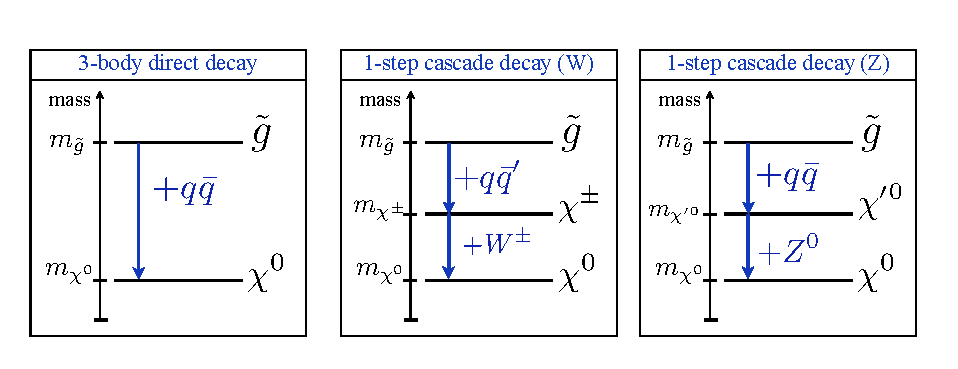
\includegraphics[width=\textwidth]{fig/gluino_sms_decays}
\caption{Illustration of the gluino decay modes within the T1 simplified model
  topology. \cite{alves_simplified_2011}}
\label{fig:gluino_sms_decays}
\end{figure}

In most \ac{mSUGRA} or \ac{GMSB} models, the $\PSgxzi \approx \PSB$ and there is
not a strong left-right mass splitting in the squarks. Therefore, it is unlikely
for the direct decays to dominate. In most cases, 1-step cascade decays
will be favoured. In these the, gluino decays first to either a $\PSgxpm$ or a
heavy $\PSgxz$. This will subsequently decay via either a $\PW$ or a $\PZ$ to
the $\PSgxzi$.

\subsubsection{T2 Simplified Model Topology}
For the T2 simplified model, the produced $\tilde{Q}$ can decay as follows:
\begin{eqnarray}
\tilde{Q} &\longrightarrow \tilde{G} \Pq \label{eqn:t2gluino}\\
\tilde{Q} &\longrightarrow \tilde{X}^0_i \Pq \\
\tilde{Q} &\longrightarrow \tilde{X}^\pm_i \Pq
\end{eqnarray}
If allowed, the \ref{eqn:t2gluino} decay will dominate since it has QCD
strength.

\subsubsection{Combining Topologies}
For phenomenological purposes, each separate decay topology may be considered as
an independent simplified model. The predictions of a whole set of topologies
can then be combined by taking linear combinations. For direct comparison
against experimental data, it is desirable to simulate a desired set of
topologies within a monte-carlo generator by ``turning on'' the chosen physics
subprocesses. The model parameter space can be sampled by moving through a
lattice of values in the desired range. At each lattice site, a statistically
sufficient number of events is generated with the appropriate parameter values
inserted into the configuration of the \ac{MC} generator.

\section{Statistical Methods}
\subsection{Background}

\subsection{Modelling the Single Lepton Analysis}
As described in the previous section, the core component of many statistical
interpretations is the construction of an appopriate likelihood function. The
likelihood must model all statistical and systematic effects and is thus highly
dependent on the experiment. The situation is considerably complicated when
shape information is included, for which relevant bin-to-bin correlations must
be included.

\subsubsection{Notation}
It will be helpful to define some notation. In the following, a subscript index
is assumed to run over the binned variable in the analysis
(i.e. \STlep). All nuisance parameters are written as $\nu^{(i)}$ where the
superscript index is taken to run over some set of systematics
(e.g. $\nu^{\textrm{jes}}$ might represent a jet energy scale
uncertainty). Certain variables $x$ are known to have a functional dependence on a
given nuisance parameter and are written $x(\nu)$. The nominal value of this
variable, being that which is measured in \ac{MC} or in real data is denoted
$\bar{x}$.

\subsubsection{The Likelihood Function}
In constructing the likelihood, we start by writing down the number of events
expected for each bin (assigned the index $i=0,1,2...$):
\begin{equation}
\NExpi = \NSigi(\mu, \nu^{(j)}) +
\NBkgi(\nu^{(k)}) \\
\end{equation}
where \NSigi is the expected signal yield for a chosen
signal model and \NBkgi is the data-driven background
prediction. As can be seen, the signal yield is a function of the \ac{poi} (the
signal strength) and some number of nuisance parameters where the index $j$
will run over a set of systematics relevant to the signal yield. Ignoring
signal contamination effects (which will be discussed later), the bacground
yield depends only on the nuisance parameters $\nu^{(k)}$ where $k$ is taken to run
over the set of systematics relevant to the bacground prediction.

Without giving an explicit functional form for the signal yield and background
prediction, the form of the likelihood function may be constructed. The
likelihood must include:
\begin{enumerate}
\item Statistical terms representing the likelihood of observing the given
  number of events given a certain expectation for the signal and background
  yields.
\item Terms providing prior constraints on the various nuisance
  parameters. Certain uncertainties are statistical in nature and thus,
  indepdent nuisance parameters are assigned per bin along with a corresponding
  prior pdf. In other cases, the underlying systematic variation is considered
  to have a 100\% correlated effect across the bins. In these cases, a single
  nuisance parameter and prior pdf is assigned.
\end{enumerate}

The form of the likelihood is as follows,
\begin{equation}
\mathcal{L} = \prod_i \Poisson(\NExpi ; \NObsi)
\prod_{\alpha \in \Theta}  X_\alpha(\nu^{(\alpha)})
\end{equation}
where
\begin{itemize}
\item $\mathcal{P}(\mu;x)$ denotes a Poisson distribution with mean $\mu$ and value
$x$
\item The $X_\alpha(\nu^{(\alpha)})$ represent some prior pdf associated with
  each systematic $\alpha$.
\end{itemize}

\subsubsection{The Signal Yield}
The signal yield per bin is constructed as follows
\begin{equation}
\NSigi = \mu \times \epsilon_i(\nu^{(\alpha)}) \times \sigma \times L \times \nu^{\textrm{lumi}}
\end{equation}

with
\begin{itemize}
\item $\epsilon_i(\nu^{(\alpha)})$ is the efficiency of the $i$th bin assumed to be
  dependent on a set of nuisance parameters $\nu^{(\alpha)}$.
\item $\sigma$ the cross-section of the signal model being considered,
\item $L$ the integrated luminosity,
\item $\nu^{\textrm{lumi}}$ the nuisance parameter associated with uncertainty in the
estimate of the integrated luminosity.
\end{itemize}

\subsubsection{Background Prediction}
The background prediction per bin is then written as
\begin{equation}
\NBkgi = \RCSi(\nu_i^{(\alpha)}, \nu^{(\beta)}) \times \NControli(\nu_i^{(\gamma)})
\end{equation}
where
\begin{itemize}
\item \RCSi is the translation ratio as defined in Section TODO,
\item The nuisance parameters $\nu_i^{(\alpha)}$ and $\nu_i^{\gamma}$ represent
  statistical uncertainties uncorrelated between the bins.
\item The nuisance parameters $\nu_i^{(\beta)}$ represent systematic
  uncertainties assumed to be 100\% correlated across the bins.
\item \NControli the observed number of events in the control region
($L_P > 0.3$)
\end{itemize}

\subsubsection{Parameterising Systematics}
In reality, it is almost always impossible to obtain a full functional form for
a variable $x$ (e.g. \RCSi, \NControli) in terms of a set of nuisance parameters
$\nu^{(\alpha)}$. Writing the Taylor expansion of $x(\nu^{(\alpha)})$ for two terms to
second order,
\begin{align*}
 x(\nu^{(A)}, \nu^{(B)})\bigg|_{\substack{\nu^{(A)} = a\\ \nu^{(B)} = b}} \approx
x(a,b) +
(\nu^{(A)} - a)\left.\frac{\partial x}{\partial\nu^{(A)}}\right|_{\nu^{(A)}=a} +
(\nu^{(B)} - b)\left.\frac{\partial x}{\partial\nu^{(B)}}\right|_{\nu^{(B)}=b} +\\
\frac{1}{2!}\left[
(\nu^{(A)} - a)^2 \frac{\partial^2 x}{\partial \left(\nu^{(A)}\right)^2}
+ (\nu^{(B)} - b)^2 \frac{\partial^2 x}{\partial \left(\nu^{(B)}\right)^2}
+ 2(\nu^{(A)} - a)(\nu^{(B)} - b)\frac{\partial^2 x}{\partial
  \nu^{(A)}\partial\nu^{(B)}}
\right]
\end{align*}
Assuming the expansion is performed with respect to the mean of x, $\bar{x}$,
the values of $a$ and $b$ are seen to be the mean values of the corresponding nuisance
parameters. For small deviations from the mean,
\begin{equation}
 (\nu^{(A)} - a) \sim (\nu^{(B)} - b) \sim \epsilon \sim 0
\end{equation}
and ignoring terms $O(\epsilon^2)$

\begin{equation}
x(\nu^{(A)}, \nu^{(B)}) \approx \bar{x} +
(\nu^{(A)} - a)\left.\frac{\partial x}{\partial\nu^{(A)}}\right|_{\nu^{(A)}=a} +
(\nu^{(B)} - b)\left.\frac{\partial x}{\partial\nu^{(B)}}\right|_{\nu^{(B)}=b}
\label{eqn:stats:taylor}
\end{equation}
Since the derivatives in Equation~\ref{eqn:stats:taylor} will in practice be
derived from some finite variation of the underlying quantity associated with
each nuisance parameter, the infinitessimal derivatives must be replaced by
finite changes. It is also sensible to set $a=b=0$.
\begin{equation}
x(\nu^{(A)}, \nu^{(B)}) \approx \bar{x} +
\nu^{(A)}\frac{\Delta x}{\Delta\nu^{(A)}} +
\nu^{(B)}\frac{\Delta x}{\Delta\nu^{(B)}}
\label{eqn:stats:taylor2}
\end{equation}
Since the value of $x$ is often associated with a physical quantity such as an
efficiency or an event yield, it is desirable to constrain it to positive
values. This can be achieved providing the range of each nuisance parameter is
set such that
\begin{equation}
\nu^{(\alpha)}\times\frac{\Delta x}{\Delta \nu^{(\alpha)}} < \bar{x}
\end{equation}

The previous derivation can be simply extended two $N > 2$ nuisance
parameters. Generalising and rewriting Equation~\ref{eqn:stats:taylor2},
\begin{eqnarray*}
x(\nu^{(A)}, \nu^{(B)}, \ldots) &\approx& \bar{x} +
\nu^{(A)}\frac{\Delta x}{\Delta\nu^{(A)}} +
\nu^{(B)}\frac{\Delta x}{\Delta\nu^{(B)}} + \ldots \\
&\approx& \frac{1}{\bar{x}^{N-1}} \left\{ \bar{x}^N +
\bar{x}^{N-1} \nu^{(A)}\frac{\Delta x}{\Delta\nu^{(A)}} +
\bar{x}^{N-1} \nu^{(B)}\frac{\Delta x}{\Delta\nu^{(B)}} + \ldots \right\}
\end{eqnarray*}
Trying to rewrite as a product,
\begin{eqnarray*}
\prod_{j=A, B, \ldots} \left(\bar{x} + \frac{\Delta x}{\Delta\nu^{(\alpha)}}\right) &=&
\bar{x}^N + \bar{x}^{N-1} \sum_{j=A, B, \ldots} \nu^{(\alpha)}\frac{\Delta x}{\Delta \nu^{(\alpha)}} \\
&&+ \bar{x}^{N-2}\sum_{j=A, B, \ldots} \sum_{k=A, B, \ldots} \nu^{(\alpha)}\nu^{(\beta)}\frac{\Delta x}{\Delta
  \nu^{(\alpha)}}\frac{\Delta x}{\Delta \nu^{(\beta)}} \\
&&+ \ldots +O(\nu^N)
\end{eqnarray*}
Ignoring terms greater than $O(\nu^2)$,
\begin{eqnarray*}
\prod_{j=A, B, \ldots} \left(\bar{x} + \frac{\Delta x}{\Delta\nu^{(\alpha)}}\right) &\approx&
\bar{x}^N + \bar{x}^{N-1} \sum_{j=A, B, \ldots} \nu^{(\alpha)}\frac{\Delta x}{\Delta
  \nu^{(\alpha)}} \\
&\approx& \bar{x}^{N-1} x(\nu^{(A)}, \nu^{(B)}, \ldots)
\end{eqnarray*}
and therefore
\begin{equation}
x(\nu^{(A)}, \nu^{(B)}, \ldots) \approx \frac{1}{\bar{x}^{N-1}} \prod_{j = A, B,
  \ldots} \left(\bar{x} + \frac{\Delta x}{\Delta\nu^{(\alpha)}}\right) \approx
\bar{x} \prod_{j = A, B,
  \ldots} \frac{1}{\bar{x}}\left(\bar{x} + \frac{\Delta x}{\Delta\nu^{(\alpha)}}\right)
\label{eqn:stats:systderiv}
\end{equation}

Using Equation~\ref{eqn:stats:systderiv}, the signal yield can be rewritten as follows
\begin{equation}
\NSigi = \mu \times \bar{\epsilon}_i \times \prod_{j}\left(\frac{\bar{\epsilon}_i
    + \nu^{(\alpha)}\frac{\Delta\epsilon_i}{\Delta\nu^{(\alpha)}}}{\bar{\epsilon}_i}\right) \sigma \times L \times \nu^{\textrm{lumi}}
\end{equation}
and the background prediction
\begin{equation}
\NBkgi = \RbarCS_i \times \prod_{j}\left( \frac{\RbarCS_i
    + \nu^{(\alpha)}\frac{\Delta\RCSi}{\Delta\nu^{(\alpha)}}}{\RbarCS_i}\right)
\times \NbarControl_i \times \prod_{k}\left( \frac{\NbarControl_i
    + \nu^{(\alpha)}\frac{\Delta\NControli}{\Delta\nu^{(\beta)}}}{\NbarControl_i}\right)
\end{equation}

\subsection{Nuisance Parameters}
The nuisance parameters incorporated in the model described thus far are of two
types.
\begin{enumerate}
\item Statistical uncertainties assumed to be uncorrelated across analysis
  bins. This includes uncertainties arising from limited generator statistics,
  limited data in the control region and signal contamination in the control
  region.
\item Systematic uncertainties arising from detector artefacts or theoretical
  uncertainties such as jet energy scale, standard model cross-sections and
  integrated luminosity measurement.
\end{enumerate}
For uncertainties of the first kind, independent nuisance paramters must be
included for each analysis bin. For uncertainties of the second kind, a
single nuisance parameter will be included for all bins. This achieves the
desired correlation. A full list of the nuisance parameters used is shown in
Table~\ref{tbl:systematic_parameters}.

\ctable[
cap=Nuisance parameters included in the single lepton likelihood function,
caption=Summary of nuisance parameters included in the single lepton likelihood function.,
mincapwidth=0.5\textwidth,
label=tbl:inter_systematic_parameters,
pos=h,
doinside=\scriptsize
]{lccccc}{
\tnote[a]{Muon channel only}
\tnote[b]{Electron channel only}

\tnote[c]{In the electron channel, the use of \ac{MC} templates in the QCD
  background estimate introduces a dependence on the \ac{JES}. Whilst the
  ability to include these correlations was added to the statistics package, it
  was not used in the results shown.}

}{\FL
Uncertainty                        & Correlated & \NSigi     & \RCSi      & \NControli & Nuisance Parameters\ML
%
Luminosity                         & \checkmark & \checkmark &            &            & $\nu^{\textrm{lumi}}$\NN
\acf{JES}                          & \checkmark & \checkmark & \checkmark & \tmark[c]  & $\nu^{\textrm{jes}}$\NN
\MET Resolution                    & \checkmark & \checkmark & \checkmark & \tmark[c]  & $\nu^{\textrm{metres}}$\NN
\PW/\Ptop\APtop Ratio              & \checkmark &            & \checkmark &            & $\nu^{W\Ptop\APtop}$\NN
\PW Polarisation                   & \checkmark &            & \checkmark &            & $\nu^{\textrm{\PW pol}}$\NN
Muon Momentum Scale\tmark[a]       & \checkmark &            & \checkmark &            & $\nu^{\textrm{lep}}$\NN
Limited \ac{MC} Statistics         &            &            & \checkmark &            & $\nu^{\textrm{MC}}_i$\NN
Limited Data Statistics            &            &            &            & \checkmark & $\nu^{\textrm{data}}_i$\NN
Signal Contamination               &            &            &            & \checkmark & $\nu^{\textrm{sig cont}}_i$\NN
\ac{PDF} Uncertainties             & \checkmark & \checkmark &            &            & $\nu^{\textrm{pdf}}_i$\NN
QCD Background Prediction\tmark[b] &            &            &            & \checkmark & $\nu^{\textrm{qcd}}_i$\LL
}

\subsection{Signal Contamination}
It can be seen in Figure~TODO that the region \LPcontrol may have a substantial
component of \ac{SUSY} events depending on the particular model under
consideration. Signal contamination increases \NControl leading to an
overprediction of \NBkg. To account for this, the \NBkgi term is modifed to
reflect the assumption that some fraction of the yield \NControli will be
due to \ac{SUSY} contamination. Rewriting,

\begin{equation}
\NBkgi(\mu, \nu^{(\alpha)}) = \RbarCS_i \times \prod_{j}\left( \frac{\RbarCS_i
    + \nu^{(\alpha)}\frac{\Delta\RCSi}{\Delta\nu^{(\alpha)}}}{\RbarCS_i}\right)
\times \NbarControl_i \times f^{\textrm{SM}}_i(\mu) \times \prod_{k}\left( \frac{\NbarControl_i
    +
    \nu^{(\alpha)}\frac{\Delta\NControli}{\Delta\nu^{(\beta)}}}{\NbarControl_i}\right)
\label{eqn:bgprediction}
\end{equation}
where $f^{\textrm{SM}}_i$ represents the fraction of \NControli expected to be
\ac{SM} events given the current signal hypothesis i.e.
\begin{equation}
f^{\textrm{SM}}_i(\mu) = \frac{\NSMi}{\NSMi + \NSUSYi(\mu)}
\end{equation}
The expected number of \ac{SUSY} events $\NSUSYi =
\mu\times\epsilon^{\textrm{control}}_i\times\sigma\times L$ where
$\epsilon^{\textrm{control}}_i$ is the efficiency calculated for \ac{SUSY}
events entering the \LPcontrol control region. To reflect these constraints, we
setup an appropriate prior distribution
\begin{equation}
X(\nu^{\textrm{SM}}) = \Gauss \left( \frac{\NSMi}{\NSMi + \mu\times\epsilon_i^{\textrm{control}}\times\sigma\times L}
; \nu^{\textrm{SM}} \right)
\end{equation}
and $f^{\textrm{SM}}_i \equiv \nu^{\textrm{SM}}_i$. Calculating the expected value of the nuisance parameter,
\begin{eqnarray}
<f^{\textrm{SM}}_i> &=& \frac{\NSMi}{\NSMi + \mu\NSUSYi} \\
                   &=& \frac{1}{1 + \mu\frac{\NSUSYi}{\NSMi}}
\label{eqn:fSMideal}
\end{eqnarray}
Technical problems associated with adding a functional dependence on the
\ac{poi} $\mu$ to the mean of the prior distribution necessitated a slightly
altered formulation. As will be shown, this formulation is approximately
equivalent given certain assumptions about the range of $\mu$ and the degree of
signal contamination. The prior distribution included in \likelihood is
rewritten as
\begin{equation}
X(\nu^{\textrm{SM}}_i) = \Gauss \left( \frac{\NSMi}{\NSMi + \epsilon_i^{\textrm{control}}\times\sigma\times L}
; \nu^{\textrm{SM}}_i \right)
\end{equation}
The term included in the background prediction (\ref{eqn:bgprediction}) is modified to
\begin{equation}
f^{\textrm{SM}}_i = 1 - \mu \times \left(1- \nu^{\textrm{SM}}_i\right)
\end{equation}
It can be seen that for $\mu=0$, $f^{\textrm{SM}}_i=1$ and for $\mu=1$,
$f^{\textrm{SM}}_i=\nu^{\textrm{SM}}_i$ as required. It will now be shown that
for a suitable range of $\mu$ and for small values of $\NSUSYi/\NControli$, the
expectation value of $f^{\textrm{SM}}_i$ will be equivalent to
Equation~\ref{eqn:fSMideal}.
\begin{eqnarray*}
<f^{\textrm{SM}}_i> &=& 1 - \mu \times \left(1-<\nu^{\textrm{SM}}>\right) \\
                  &=& 1 - \mu  + \mu\frac{\NSMi}{\NSMi + \NSUSYi} \\
                  &=& \frac{(1-\mu)\left(\NSMi + \NSUSYi\right) + \mu\NSMi}{\NSMi + \NSUSYi} \\
                  &=& \frac{\NSMi + (1 - \mu)\NSUSYi}{\NSMi + \NSUSYi} \\
                  &=& \frac{\NSMi \left( 1 + (1-\mu)\frac{\NSUSYi}{\NSMi}\right)}{\NSMi + \NSUSYi} \\
                  &=& \frac{\NSMi}{\left(\NSMi +\NSUSYi\right)\left( 1 + (1 - \mu)\frac{\NSUSYi}{\NSMi}\right)^{-1}} \\
                  &\approx& \frac{\NSMi}{\left(\NSMi +\NSUSYi\right)\left( 1 - (1-\mu)\frac{\NSUSYi}{\NSMi}\right)} \\
                  &=& \frac{\NSMi}{\NSMi + \mu\NSUSYi - (1-\mu)\frac{\NSUSYi^2}{\NSMi}}\\
                  &=& \frac{1}{1 + \mu\frac{\NSUSYi}{\NSMi} - (1-\mu)\left(\frac{\NSUSYi}{\NSMi}\right)^2} \\
                  &\approx& \frac{1}{1 + \mu\frac{\NSUSYi}{\NSMi}}
\end{eqnarray*}

\subsubsection{Uncertainties on \NControli}
The dominant systematic uncertainty relating to the \LPcontrol region yield
arises from the limited statistics of the sample. This is especially true at
high \STlep. Accordingly, a nuisance parameter is added to the likelihood and
assigned a Gaussian prior with a width derived assuming a Poisson error on the
\NControli yield.

An additional complication arises in the case of the electron channel where the
\LPcontrol region has a non-negligible component of \ac{QCD} multijet
events. These are unreliably modelled by event generators and thus not included
in the calculation of \RCSi. This additional contribution to \NControli would
again lead to an overprediction of the background. To correct this, an
additional factor is included in Equation~\ref{eqn:bgprediction},
$f^{\textrm{ewk}}_i$ derived from the results of the \ac{QCD} fit detailed in
Section~TODO. The error derived from the fit procedure is modelled as a
Gaussian prior on an additional nuisance parameter $\nu^{\textrm{QCD}}_i$. It
has been assumed, and confirmed by the results of the fit in data that the
region \LPsignal is \ac{QCD} free.

The uncertainty included via the prior distribution of $\nu^{\textrm{QCD}}$ was
the quadrature sum of the statistical error from the fitting procedure and an
uncertainty accounting for the limited generator statistics used to construct
the fit templates. Additional errors coming from jet energy scale uncertainty
and missing energy resolution were found to be small. Proper inclusion of these
into the likelihood would need to ensure correlation with the nuisance
parameters representing these uncertainties. The relevant terms were setup but
not included in the final calculations. The contribution is seen to be small and
unnecessary complication of the likelihood function tends to increase the
processing time, especially when running a large number of toy experiments.


\section{Results}

\begin{figure}
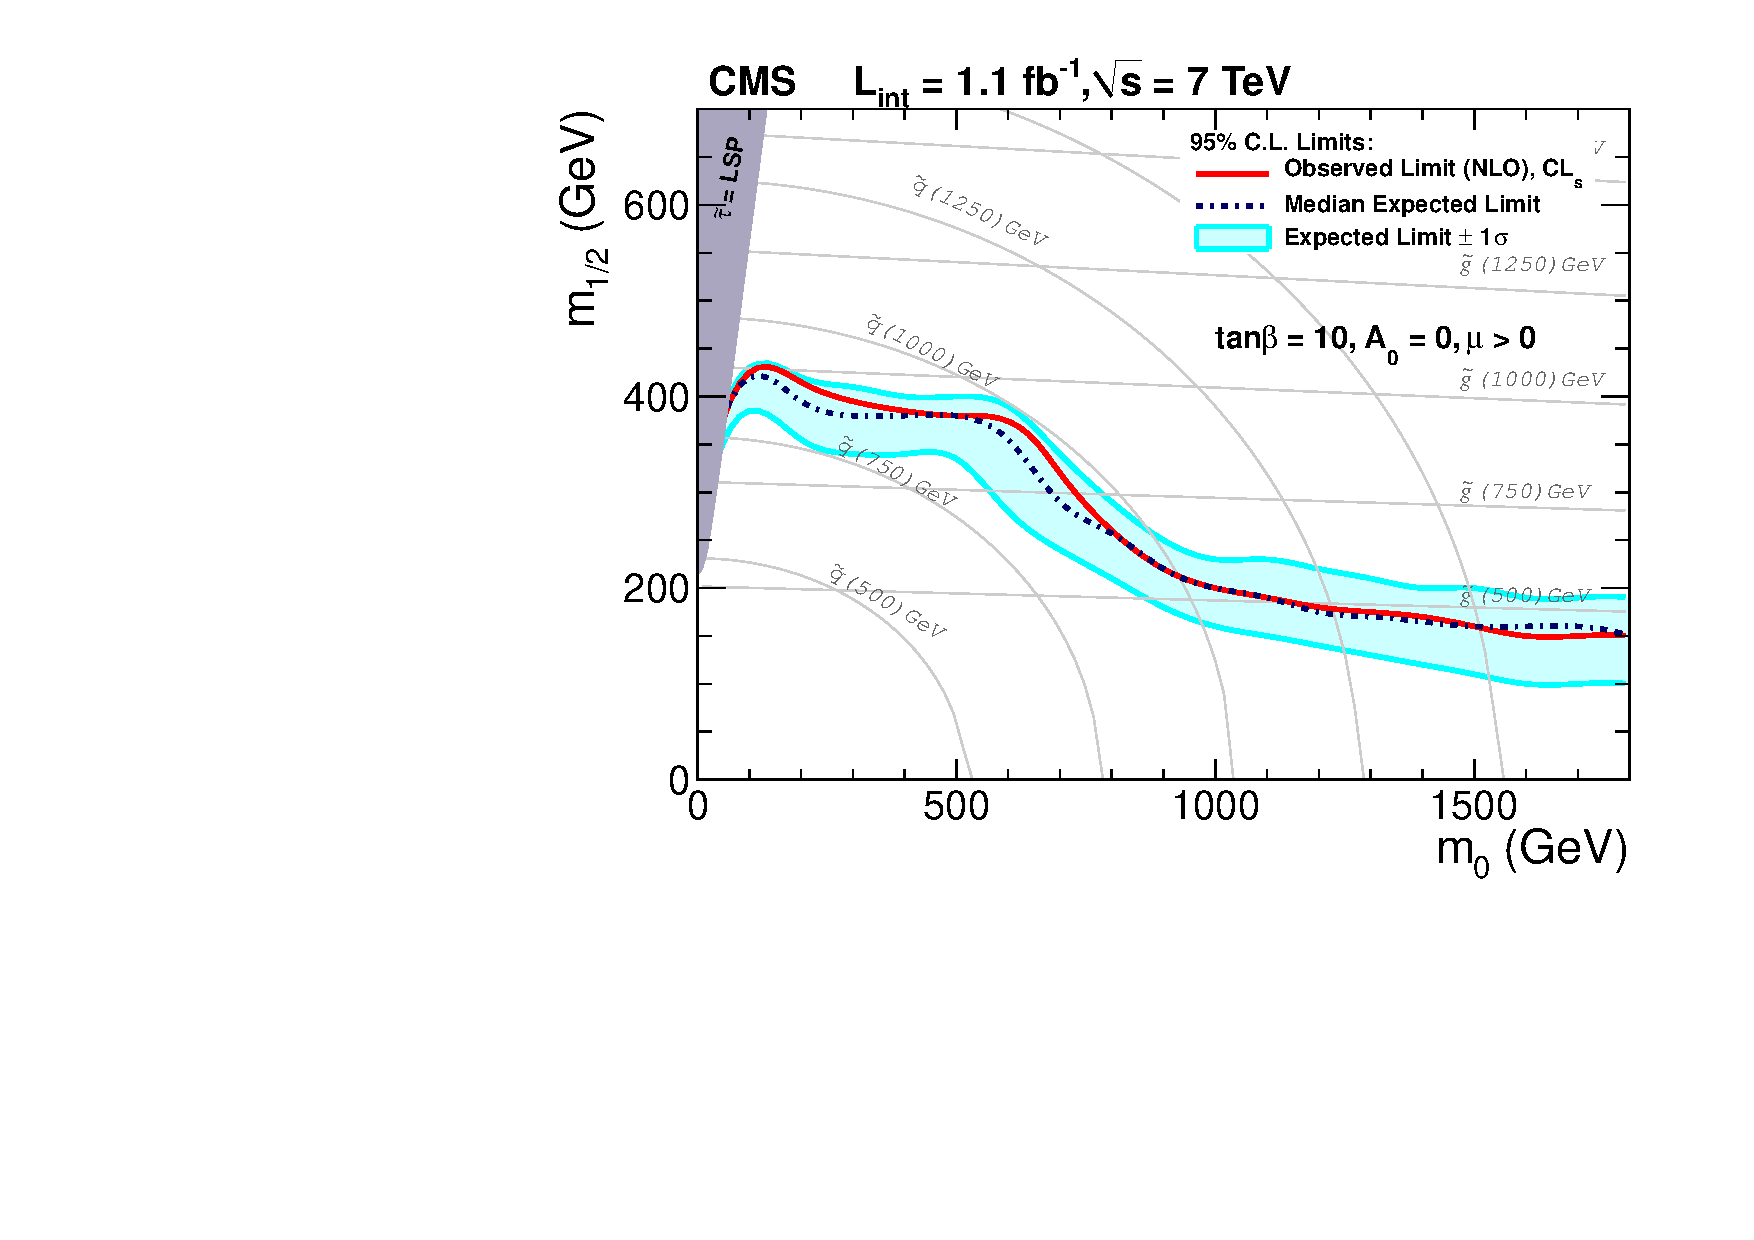
\includegraphics[width=\textwidth]{fig/RA4_ExclusionLimit_tanb10}
\end{figure}
%%% Local Variables:
%%% mode: latex
%%% TeX-master: "../thesis"
%%% End:

\end{comment}

%% Produce the appendices
\begin{appendices}
  
\chapter{Kinematics}
A Lorentz tranformation can be written as
\begin{equation}
\left(\begin{array}{c} E' \\ p_{\parallel}' \end{array} \right)
=
\left(
\begin{array}{cc}
\gamma & -\gamma\beta \\
-\gamma\beta & \gamma
\end{array}
\right)
\left (\begin{array}{c} E \\ p_{\parallel} \end{array}\right)
\end{equation}
and
\begin{equation}
p_{\perp}' = p_{\perp}
\end{equation}

Boosting from a particles rest frame into the lab frame,
\begin{equation}
\left(\begin{array}{c} E \\ P \end{array} \right)
=
\left(
\begin{array}{cc}
\gamma & -\gamma\beta \\
-\gamma\beta & \gamma
\end{array}
\right)
\left (\begin{array}{c} M \\ 0 \end{array}\right)
\end{equation}
and so
\begin{eqnarray*}
E &=& \gamma M  \Longrightarrow \gamma = \frac{E}{M} \\
|P| &=& \gamma\beta M \Longrightarrow \beta = \frac{|P|}{\gamma M} = \frac{|P|}{E}
\end{eqnarray*}
also
\begin{eqnarray*}
\gamma &=& \frac{\sqrt{P + M}}{M} \\
&=& \sqrt{1 +\left(\frac{|P|}{M}\right)^2}
\end{eqnarray*}

\end{appendices}

%% Produce the un-numbered back matter (e.g. colophon,
%% bibliography, tables of figures etc., index...)
\begin{backmatter}
  \bibliographystyle{lucas_unsrt}
\bibliography{shorttitles,bibstrings,thesis}

\begin{colophon}
  A number of software tools were vital to the production of this thesis. The
  author is extremely grateful to the many individiuals responsible. Without
  such high-quality tools, this work would simply not have been possible.

The thesis was written using the \textsc{Emacs} text-editor and typeset with
\TeX/\LaTeX using the \textsc{HEPThesis} package. The \texttt{git} version
control system was invaluable for maintaining backups and managing changes.

All work was performed using the \textsc{GNU/Linux} operating system, primarily
the variant assembled by the volunteers of the \textsc{Arch Linux} project. Much
of the code was written using the \textsc{Python} programming language. Whilst
some plots were produced using the \textsc{ROOT} framework, the author
recommends \texttt{matplotlib} for its superior API and powerful features.
\end{colophon}

\end{backmatter}

%% Close
\end{document}

;; %%% Local Variables:
;; %%% TeX-command-default: "SCons"
;; %%% mode: latex
;; %%% TeX-PDF-mode: t
;; %%% TeX-master: "thesis"
;; %%% End:
